\documentclass[a4paper]{amsart}

\usepackage[french]{babel}
\usepackage{graphicx}
\usepackage{float}
\usepackage[export]{adjustbox} % http://ctan.org/pkg/adjustbox

% === Pour retirer l'espace énorme entre le texte et les figures ===
\usepackage{etoolbox}
\BeforeBeginEnvironment{figure}{\vskip-2ex}
\AfterEndEnvironment{figure}{\vskip-1ex}
% ==================================================================

\newtheorem{theorem}{Théorème}[section]
\newtheorem{lemma}[theorem]{Lemme}
\newtheorem{conjecture}[theorem]{Conjecture}

\theoremstyle{definition}
\newtheorem{definition}[theorem]{Définition}
\newtheorem{example}[theorem]{Exemple}
\newtheorem{xca}[theorem]{Exercice}

\theoremstyle{remark}
\newtheorem{remark}[theorem]{Remarque}

\numberwithin{equation}{section}

%    Absolute value notation
\newcommand{\abs}[1]{\lvert#1\rvert}

%    Blank box placeholder for figures (to avoid requiring any
%    particular graphics capabilities for printing this document).
\newcommand{\blankbox}[2]{%
  \parbox{\columnwidth}{\centering
%    Set fboxsep to 0 so that the actual size of the box will match the
%    given measurements more closely.
    \setlength{\fboxsep}{0pt}%
    \fbox{\raisebox{0pt}[#2]{\hspace{#1}}}%
  }%
}

\renewcommand*{\overrightarrow}[1]{\vbox{\halign{##\cr 
  \tiny\rightarrowfill\cr\noalign{\nointerlineskip\vskip1pt} 
  $#1\mskip2mu$\cr}}}

\begin{document}

\title{$\mathbb{TFJM}^2$: Problème $\no5$, Électron libre}

\author{Bellevue (BLV)}

\begin{abstract}
  Cet article contient la résolution de nombreuses questions du problème n\textsuperscript{o}5: \og Électron libre \fg{} de la quatorzième édition du Tournoi Français
  des Jeunes Mathématiciennes et Mathématiciens. La tentative de résolution du problème est composé de théorèmes et conjectures énoncés à la suite.
  Notez que pour la résolution de certains problèmes dans un plan quelconque, nous avons utilisé un plan orthonormé.

\end{abstract}

\maketitle

\tableofcontents

\section{Introduction}

Nicolas joue en disposant d’un canon à électrons immergé dans un champ magnétique constant uniforme. À l'aide de son canon, il peut émettre un électron
circulant alors à vitesse constante en décrivant un cercle dans le sens trigonométrique, que l'on a supposé de rayon 1.

Il dispose aussi d’un bouton qui permet de faire faire demi-tour à l’électron tel qu'au moment où il appuie, la vitesse de l’électron reste la même
mais progresse dans la direction opposée.

Le coeur du problème réside dans l'optimisation entre la longueur totale de la courbe du trajet, du nombre d'appuis, ainsi que la restriction d'espace.\newpage
\section{Définitions}

\begin{definition}
  On appelle \textbf{trajet} une courbe permettant de relier deux points $A,B$ dans un plan quelconque. Voici des exemples de trajets:

  \begin{figure}[H]
    \centering
    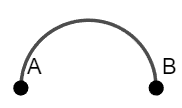
\includegraphics[scale=0.5]{images/circle.png}
    \caption{Un trajet demi-circulaire.}
  \end{figure}

  \begin{figure}[H]
    \centering
    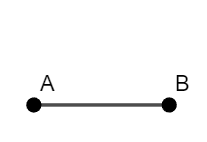
\includegraphics[scale=0.5]{images/line.png}
    \caption{Un trajet étant le segment [AB].}
  \end{figure}

  \begin{figure}[H]
    \centering
    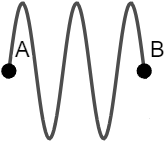
\includegraphics[scale=0.5]{images/sinus.png}
    \caption{Un trajet sinusoïdal.}
  \end{figure}

  Dans le cadre du problème, nous appellerons plus régulièrement \textbf{trajet} tel un trajet circulaire, demi-circulaire ou plus généralement un arc de cercle.
\end{definition}

\begin{definition}
  On appelle \textbf{trajet stable} un trajet (ou plusieurs petits trajets formant un plus grand trajet) inscrit dans un cercle $C_r$ de rayon $r>0$ ne touchant pas la courbe de $C_r$ (selon la Question 2).
\end{definition}

\begin{definition}
  On appelle \textbf{trajet périodique} un trajet étant inscrit dans un polygone admirable, démarrant à un point $A$ et se terminant au point $A$, dans un angle opposé à celui de départ. (dans le cadre de la Question 5).
\end{definition}

\begin{definition}
  On appelle $\lambda(A,B)$ la longueur d'une courbe (trajet) dans un plan quelconque reliant deux points $A,B$. Dans le cadre de la courbe d'une fonction continue $f:\mathbb{R}\longrightarrow \mathbb{R}, x\longmapsto f(x)$,
  on considère donc que: \[\lambda(A,B)=\int_{x_A}^{x_B} \sqrt{1+{f^\prime}(x)^2} \,dx\]

  (La démonstration est à l'annexe).
\end{definition}

\begin{definition}
  On appelle $n_{bouton}$ le nombre de fois que l'on appuie sur le bouton permettant de changer le sens du trajet.
\end{definition}

\begin{definition}
  On appelle un \textbf{demi-cercle perpétuel complet} un trajet composée de plusieurs addition d'$1/2$ circonférence d'un cercle trigonométrique (soit $\pi$). Voici une illustration ci-dessous:

  \begin{figure}[H]
    \centering
    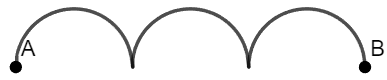
\includegraphics[scale=0.5]{images/demicircle.png}
    \caption{Un demi-cercle perpétuel complet répété trois fois.}
  \end{figure}
\end{definition}

\begin{definition}
  On appelle un \textbf{demi-cercle perpétuel} un trajet composée de plusieurs addition d'$1/2$ circonférence d'un cercle trigonométrique (soit $\pi$) en considérant aussi des arcs de cercles. Voici une illustration ci-dessous

  \begin{figure}[H]
    \centering
    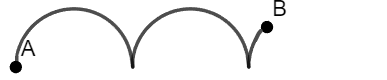
\includegraphics[scale=0.5]{images/incomplete_demi_circle.png}
    \caption{Un demi-cercle perpétuel composé de deux demi-cercle perpétuel complet et d'un dernier demi-cercle incomplet (un arc de cercle).}
  \end{figure}
\end{definition}

\begin{definition}
  On appelle \textbf{distance absolue} la plus petite distance séparant deux points $A,B$ dans un plan quelconque, soit le segment [AB] (Voir démonstration à l'annexe). On la note $d_{abs}$ avec $d_{abs}\in\mathbb{R^+}$ (une longueur étant toujours positive). On la note
  aussi $d_{abs XY}$ dans des cas particuliers hormis $A$ et $B$ (considérant donc d'autres points $X$ et $Y$).
\end{definition}

\begin{definition}
  On appelle \textbf{distance minimale} la plus petite distance séparant deux points $A,B$ dans un plan quelconque, avec un trajet circulaire (ou de demi-cercles perpétuels). On la note $d_{min}$ avec $d_{min}\in\mathbb{R^+}$ (une longueur étant toujours positive).
\end{definition}

\begin{definition}
  Pour $k,n\in\mathbb{R}$, on note $k\to n$ afin de signifier que $k$ tend vers $n$.
\end{definition}

\newpage








\section{Théorèmes pour la Question 1}

\begin{theorem}
  Dans le cas où $n_{bouton}=0$, $d_{min}= 2\arcsin (\frac{d_{abs}}{2})$
\end{theorem}

\begin{proof}
  Pouvant choisir l'orientation initiale du canon, on sait que l'on peut former un arc de cercle permettant d'atteindre $B$ à partir de $A$.
  Voici deux approches:\\

  \textbf{Approche 1}: On considère le repère orthonormé $(O;I;J)$ tel que \overrightarrow{OI} $\perp$ \overrightarrow{OJ}. On considère de même le cercle trigonométrique $C$ centré au point O et le point $A(1;0)$ inscrit dans C. Soit le point
  $B$ inscrit dans $C$ (sur sa circonférence).
  Soit $\theta$ l'angle séparant $A$ et $B$ à travers le cercle C.

  Nous pouvons donc former le triangle $\widehat{BOA}$ isocèle en $O$ avec $BO=1$, $OA=1$ et $AB=d_{abs}$. Soit $D$, milieu segment $[AB]$ tel que $OD$ coupe $\theta$ en deux. Nous avons donc deux triangles rectangles égaux $\widehat{ODA}$ et $\widehat{ODB}$.

  D'après les propriétés trigonométrique d'un triangle rectangle, nous avons:

  \[sin(\frac{\theta}{2})=\frac{d_{abs}}{2} \Leftrightarrow \theta = 2\arcsin (\frac{d_{abs}}{2})\]

  Étant dans un cercle trigonométrique, nous savons que $d_{min}=\theta$ (car $r=1$, $r$ étant le rayon du cercle), soit:
  \[d_{min}=2\arcsin (\frac{d_{abs}}{2})\] \\

  Voici une illustration géométrique de la preuve:

  \begin{figure}[H]
    \centering
    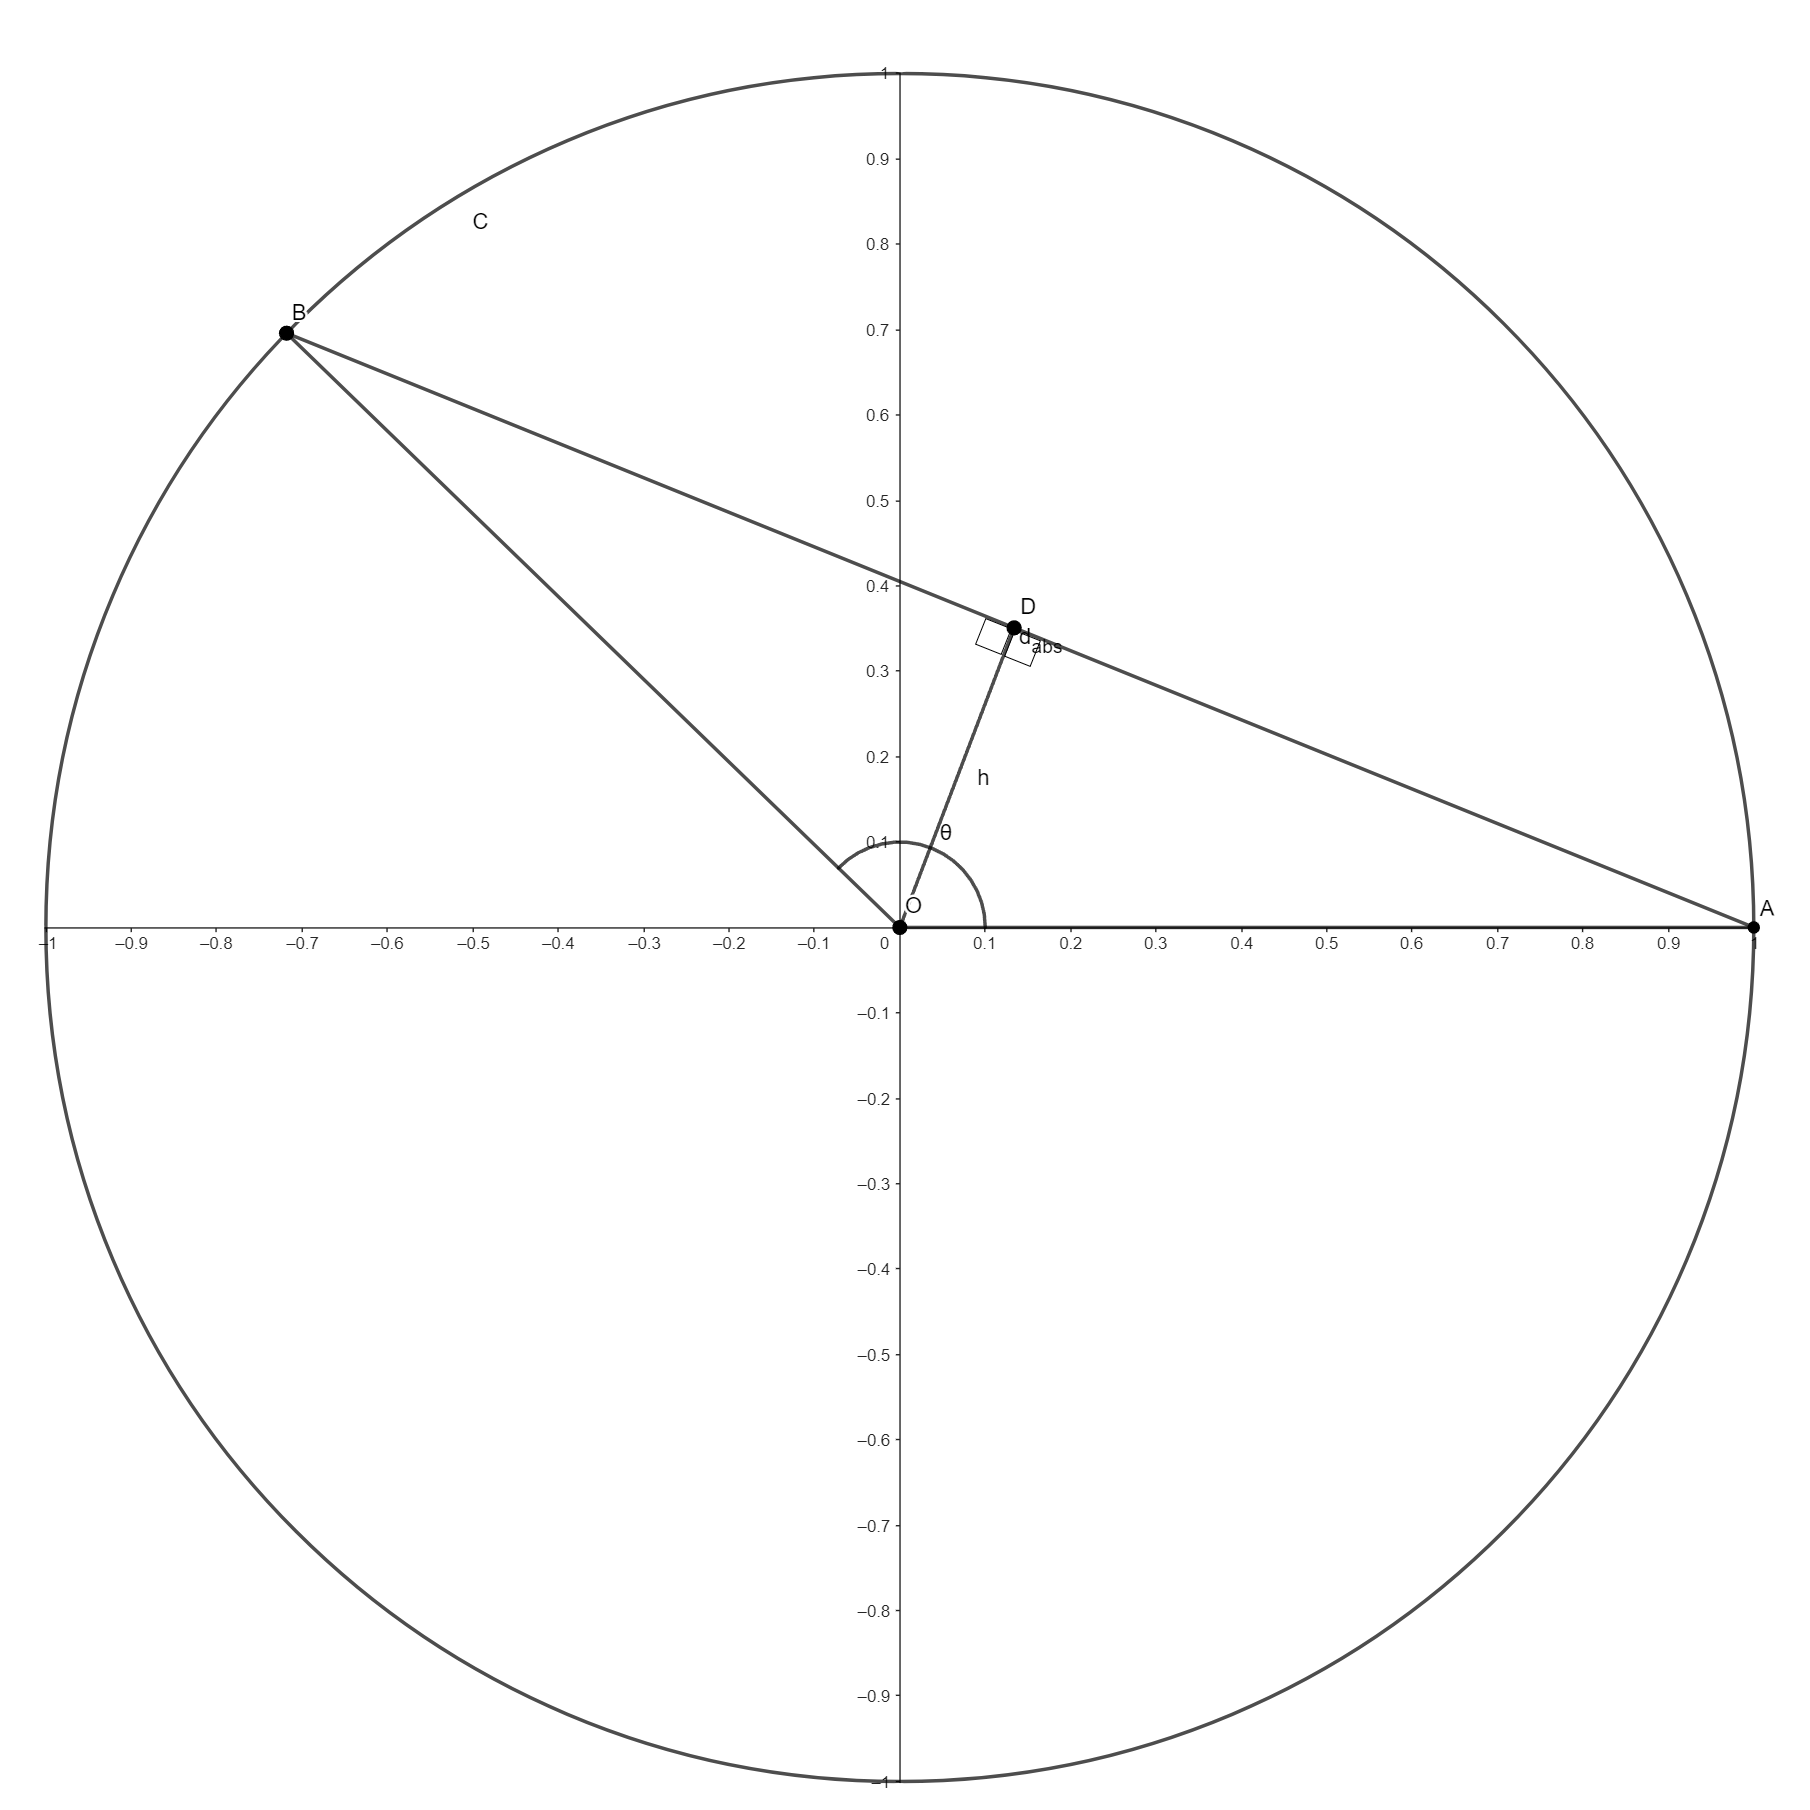
\includegraphics[scale=0.17]{images/angle.png}
    \caption{Un repère orthonormé avec le cercle trigonométrique $C$ de rayon $r=1$.}
  \end{figure}

  \textbf{Approche 2}: On considère de même le repère orthonormé $(O;I;J)$ tel que \overrightarrow{OI} $\perp$ \overrightarrow{OJ}. On considère de même le cercle trigonométrique $C$ centré au point O et le point $A(-1;0)$ inscrit dans C. Soit le point
  $B(x_B,y_B)$ inscrit dans $C$ (sur sa circonférence).

  Nous pouvons modéliser $C$ à partir de l'équation modélisant un cercle dans un repère orthonormé. Soit $r,x,y\in\mathbb{R}$ avec $y$ représentant les ordonnés, $x$ les abscisses et $r$ le rayon, tel que:
  \[r^2=y^2+x^2 \Leftrightarrow  y = \sqrt{r^2-x^2}\]

  À partir de cette égalité, nous considérons dans notre cas que $r=1$, car il s'agit du cercle trigonométrique. Nous pouvons définir la fonction $f,f:\mathbb{R}\longrightarrow [-1;1];  x\longmapsto \sqrt{1-x^2}$ .

  Voici une illustration géométrique de la courbe de $f$ ainsi que les points associés:

  \begin{figure}[H]
    \centering
    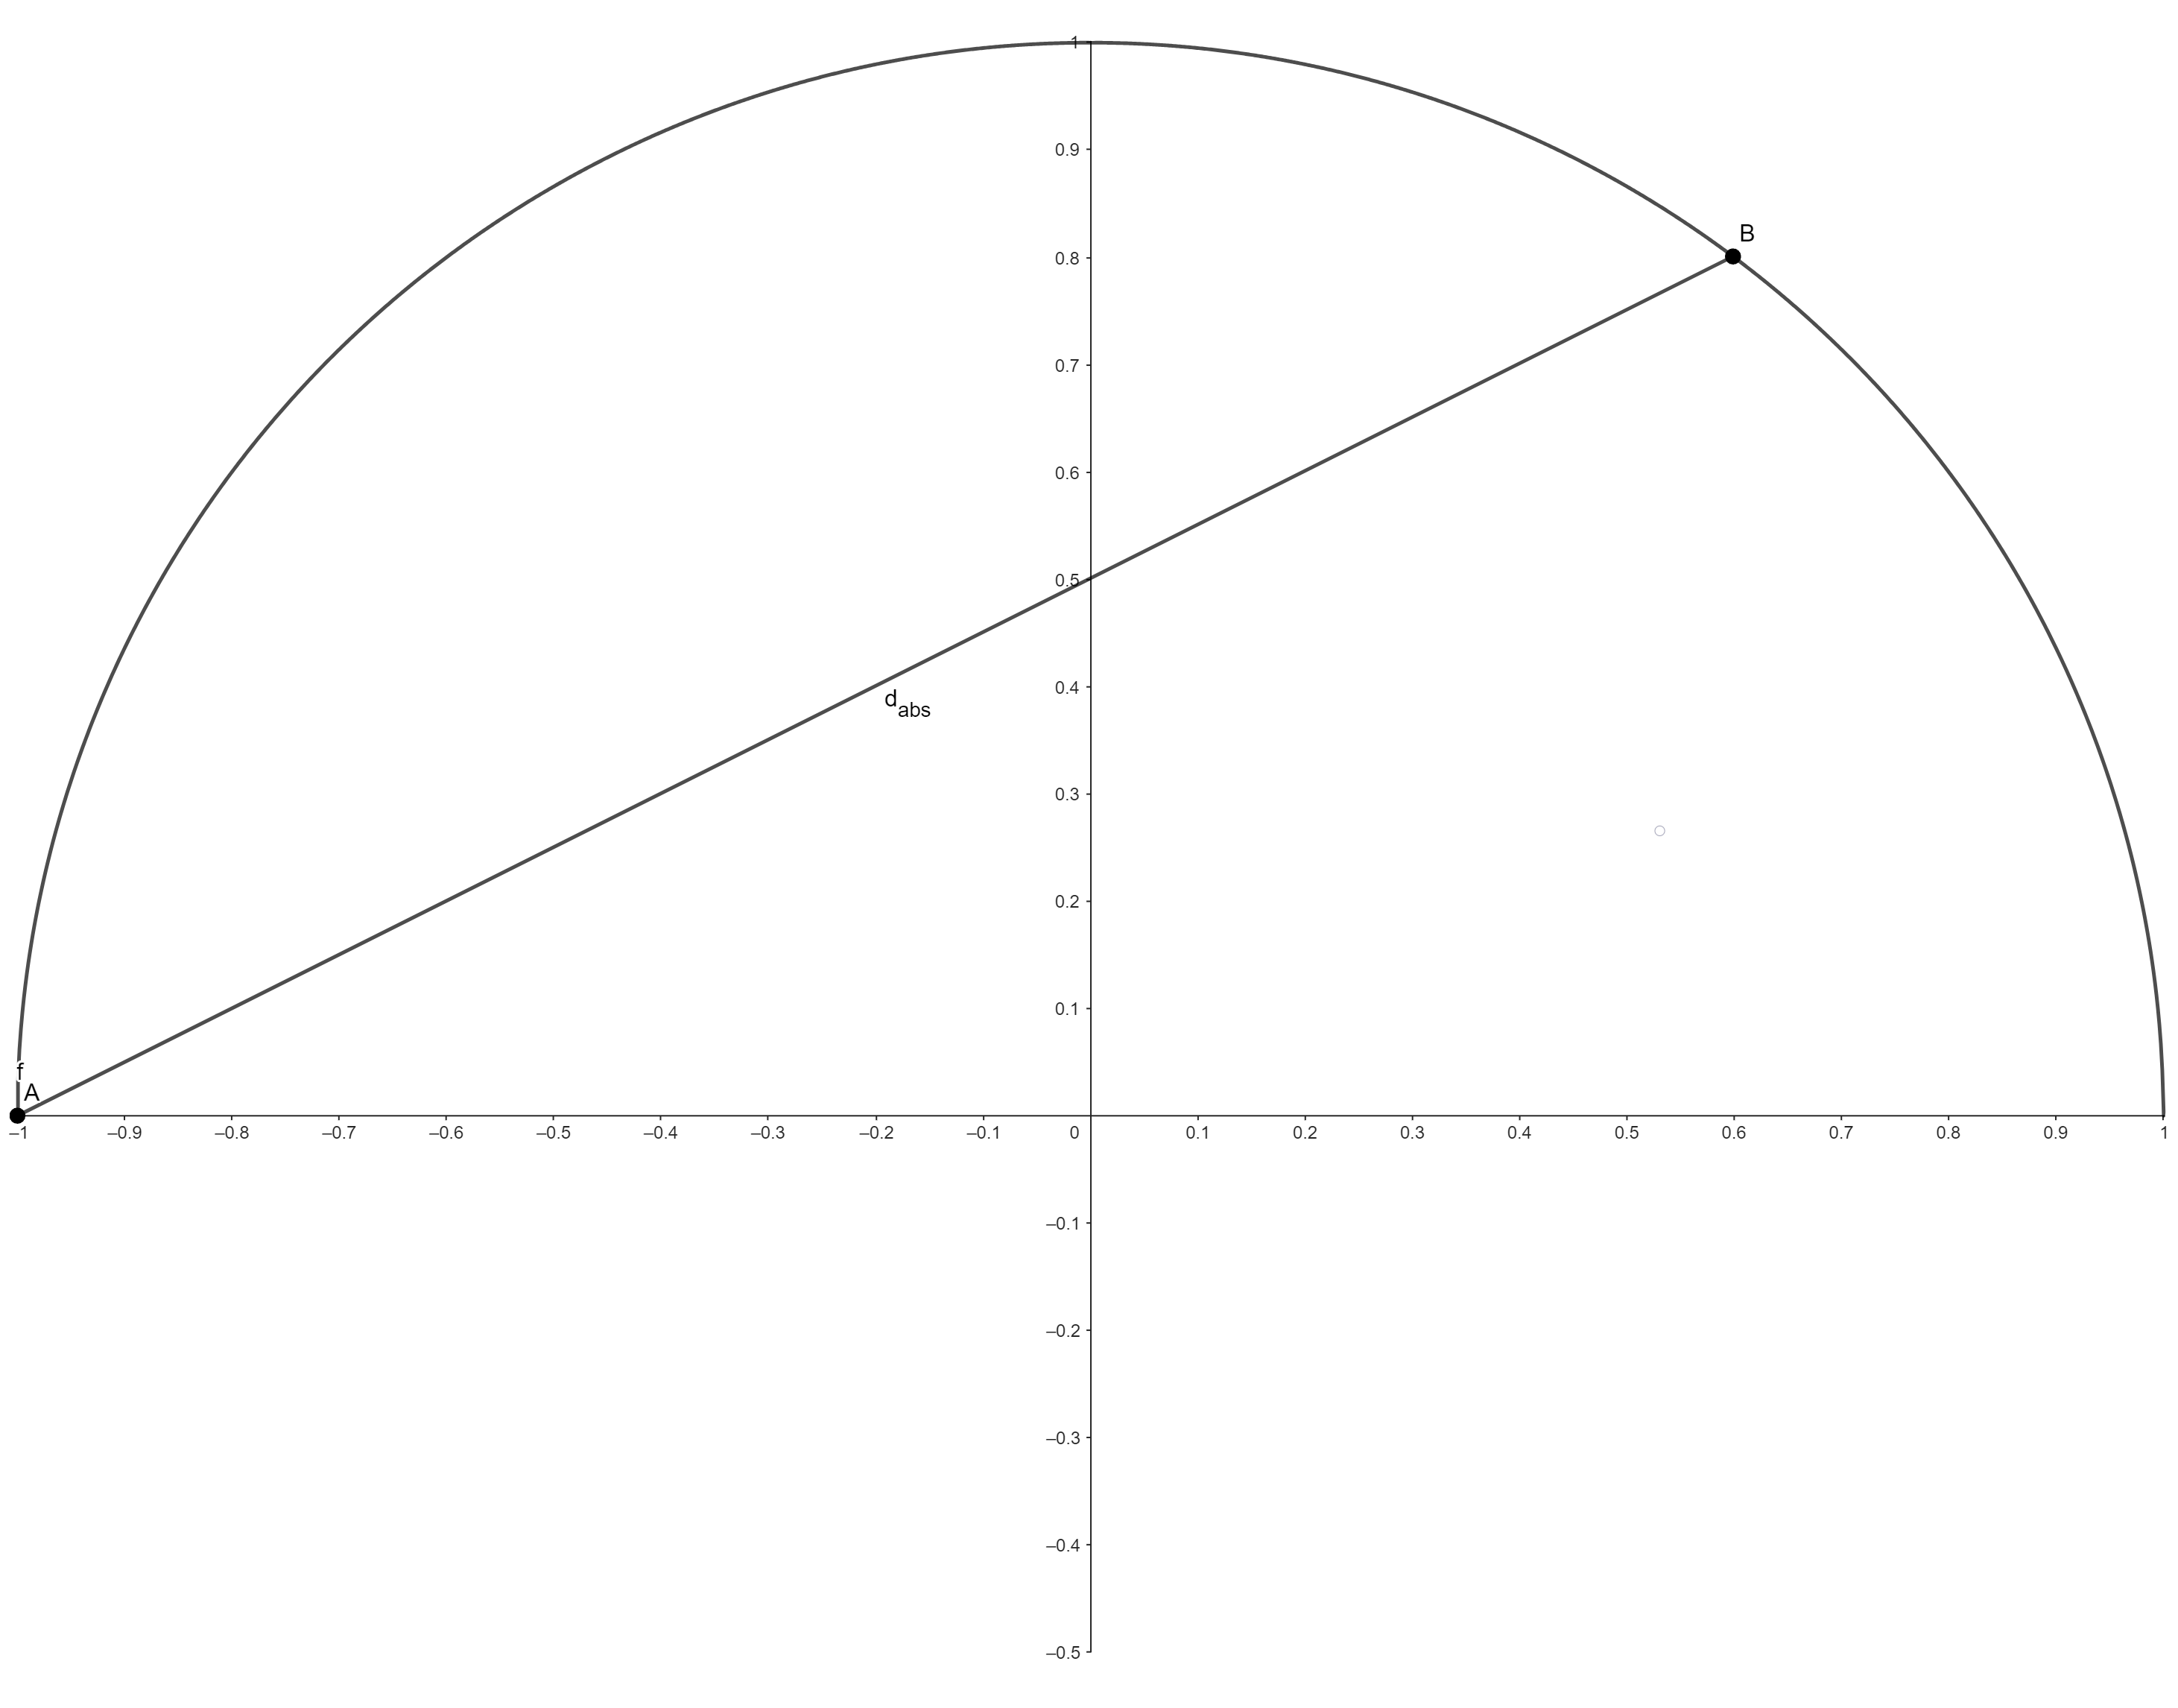
\includegraphics[scale=0.1]{images/angle_function.png}
    \caption{Représentation de $f$ avec $B(\approx0.6;\approx0.8)$.}
  \end{figure}

  Nous savons que: \[f^\prime(x)=\frac{-x}{\sqrt{1-x^2}}, \forall x\in]-1;1[\]

  Nous avons donc:

  \[d_{min}=\lambda(A,B)=\int_{-1}^{x_B} \sqrt{1+{f^\prime}(x)^2} \,dx=\int_{-1}^{x_B} \sqrt{1+(\frac{-x}{\sqrt{1-x^2}})^2}\,dx=\int_{-1}^{x_B} \frac{1}{\sqrt{1-x^2}}\,dx\]

  On admet que:

  \[\int_{-1}^{x_B} \frac{1}{\sqrt{1-x^2}}\,dx=\arcsin (x)\Biggr|_{-1}^{x_B}=\arcsin (x_B)-\arcsin (-1)\]

  Soit donc $d_{min}=\arcsin (x_B)+\frac{\pi}{2}$.

  Étant dans un repère orthonormé, nous savons aussi que, d'après le Théorème de Pythagore:

  \[{d_{abs}}^2=(x_B-x_A)^2+(f(x_B)-f(x_A))^2 \Leftrightarrow {d_{abs}}^2=2(1+x_B) \Leftrightarrow x_B=\frac{{d_{abs}}^2}{2}-1\]

  Soit donc:

  \[d_{min}=\arcsin (\frac{{d_{abs}}^2}{2}-1)+\frac{\pi}{2}\]

  Si l'on définit une fonction $f_1=d_{min}, f_1:\mathbb{R^+}\longrightarrow \mathbb{R^+}, x\longmapsto f_1(x),$ pour l'\textbf{Approche 1} et $f_2=d_{min}, f_2:\mathbb{R^+}\longrightarrow \mathbb{R^+}, x\longmapsto f_2(x),$ pour l'\textbf{Approche 2} avec $x=d_{abs}$, nous avons pour $f_1(x)=2\arcsin (\frac{x}{2})$ et $f_2(x)=\arcsin (\frac{x^2}{2}-1)+\frac{\pi}{2}$.

  En comparant les courbes des fonctions $f_1,f_2$ des deux approches, on remarque que: \[f_2(x)=\lvert f_1(x) \rvert\]

  Cela peut se justifier par le fait que l'\textbf{Approche 2} est basée sur une fonction $f(x)\geq0, \forall x\in[-1;1]$ car un carré est toujours positif. De plus, on préfèrera l'utilisation de la fonction $f_1$ car, comme $f_1$ et $f_2$
  modélisent $d_{min}$ selon $d_{abs}$, il n'est pas cohérent de considérer une longueur négative, une longueur quelconque $l\in\mathbb{R^+}$. Dans $\mathbb{R^+}$, $f_1$ et $f_2$ sont semblables. Dans tous les cas, $d_{min},d_{abs}\in\mathbb{R^+}$, donc on peut négliger cette différence.
\end{proof}

\begin{theorem}
  L'appui permettant à l'électron de progresser le plus loin dans le plan est lorsque son trajet est à la moitié de la circonférence du cercle (soit $\pi$, avec un trajet demi-circulaire, comme la Figure 1).
\end{theorem}

\begin{proof}
  Voici deux approches:\\

  \textbf{Approche 1}: Du \textbf{Théorème 3.2} découle la propriété disant que:

  \[d_{min}=2\arcsin (\frac{d_{abs}}{2}) \Leftrightarrow d_{abs}=2sin(\frac{d_{min}}{2})\]

  Soit $x=d_{min}$ et une fonction $f:\mathbb{R^+}\longrightarrow \mathbb{R^+}, x\longmapsto f(x)$ tel que  $f(x)=d_{abs}$. Nous avons donc:

  \[f(x)=2sin(\frac{x}{2})\]

  Ainsi que:

  \[f^\prime(x)=cos(\frac{x}{2})\]

  On admet que $f^\prime(x)=0$ lorsque $x=\pi$ dans l'intervalle $I=[0;2\pi]$, soit donc un maximum avec $f(\pi)=2 \Leftrightarrow d_{abs}=2$ pour $d_{min}=\pi$.

  En d'autres termes, toutes les valeurs $d_{min}$ n'amèneront pas aussi loin que son diamètre, comme $d_{abs}=2$. Cela laisse donc considérer l'idée d'appuyer sur le bouton à ce maximum afin d'effectuer un nouveau cercle trigonométrique.
  (cela laisse aussi supposer, que par récurrence, il faudra toujours appuyer sur le bouton à la moitié de la circonférence pour progresser efficacement dans le plan).\\

  \textbf{Approche 2}: En se basant plus sur de la logique, on remarque bien qu'afin d'amener notre électron le plus loin possible, il faut arrêter le trajet et appuyer sur le bouton
  au demi-cercle. En effet, si l'on appuie au délà de la circonférence, nous effectuons un trajet plus long avec une distance absolue $d_{abs}$ plus courte. Voici une illustration:

  \begin{figure}[H]
    \centering
    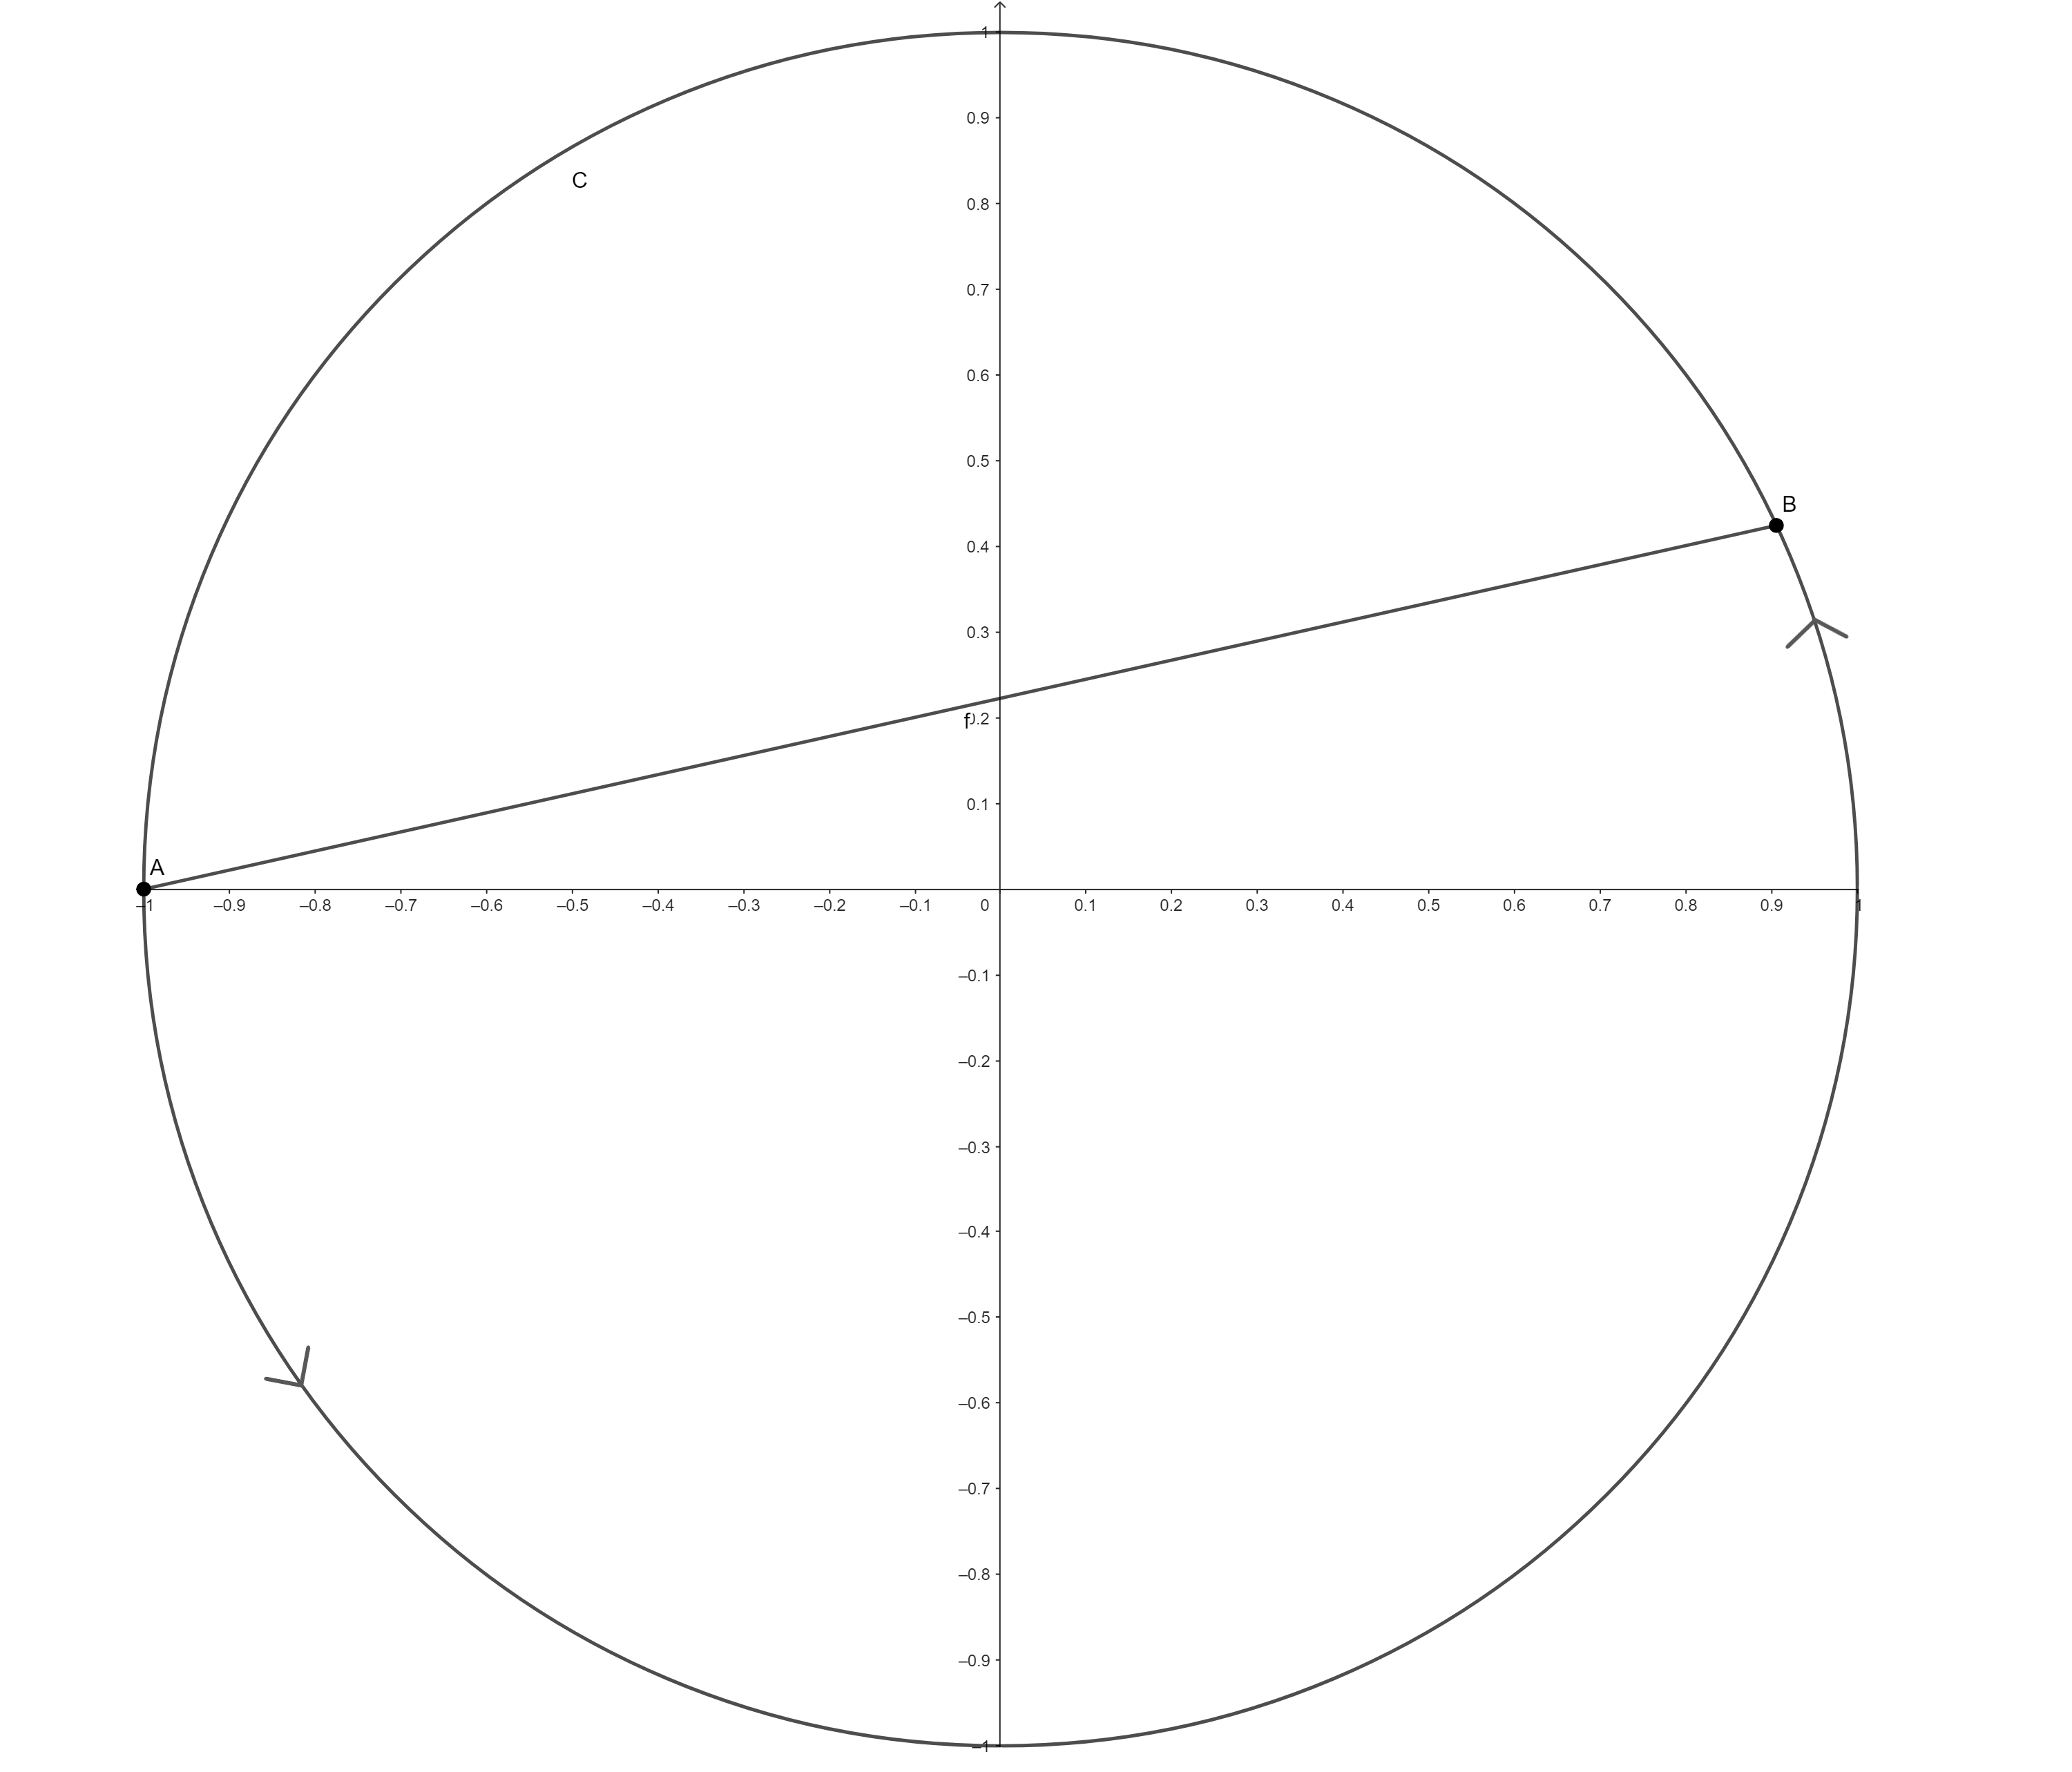
\includegraphics[scale=0.079]{images/ab_circle1.png}
    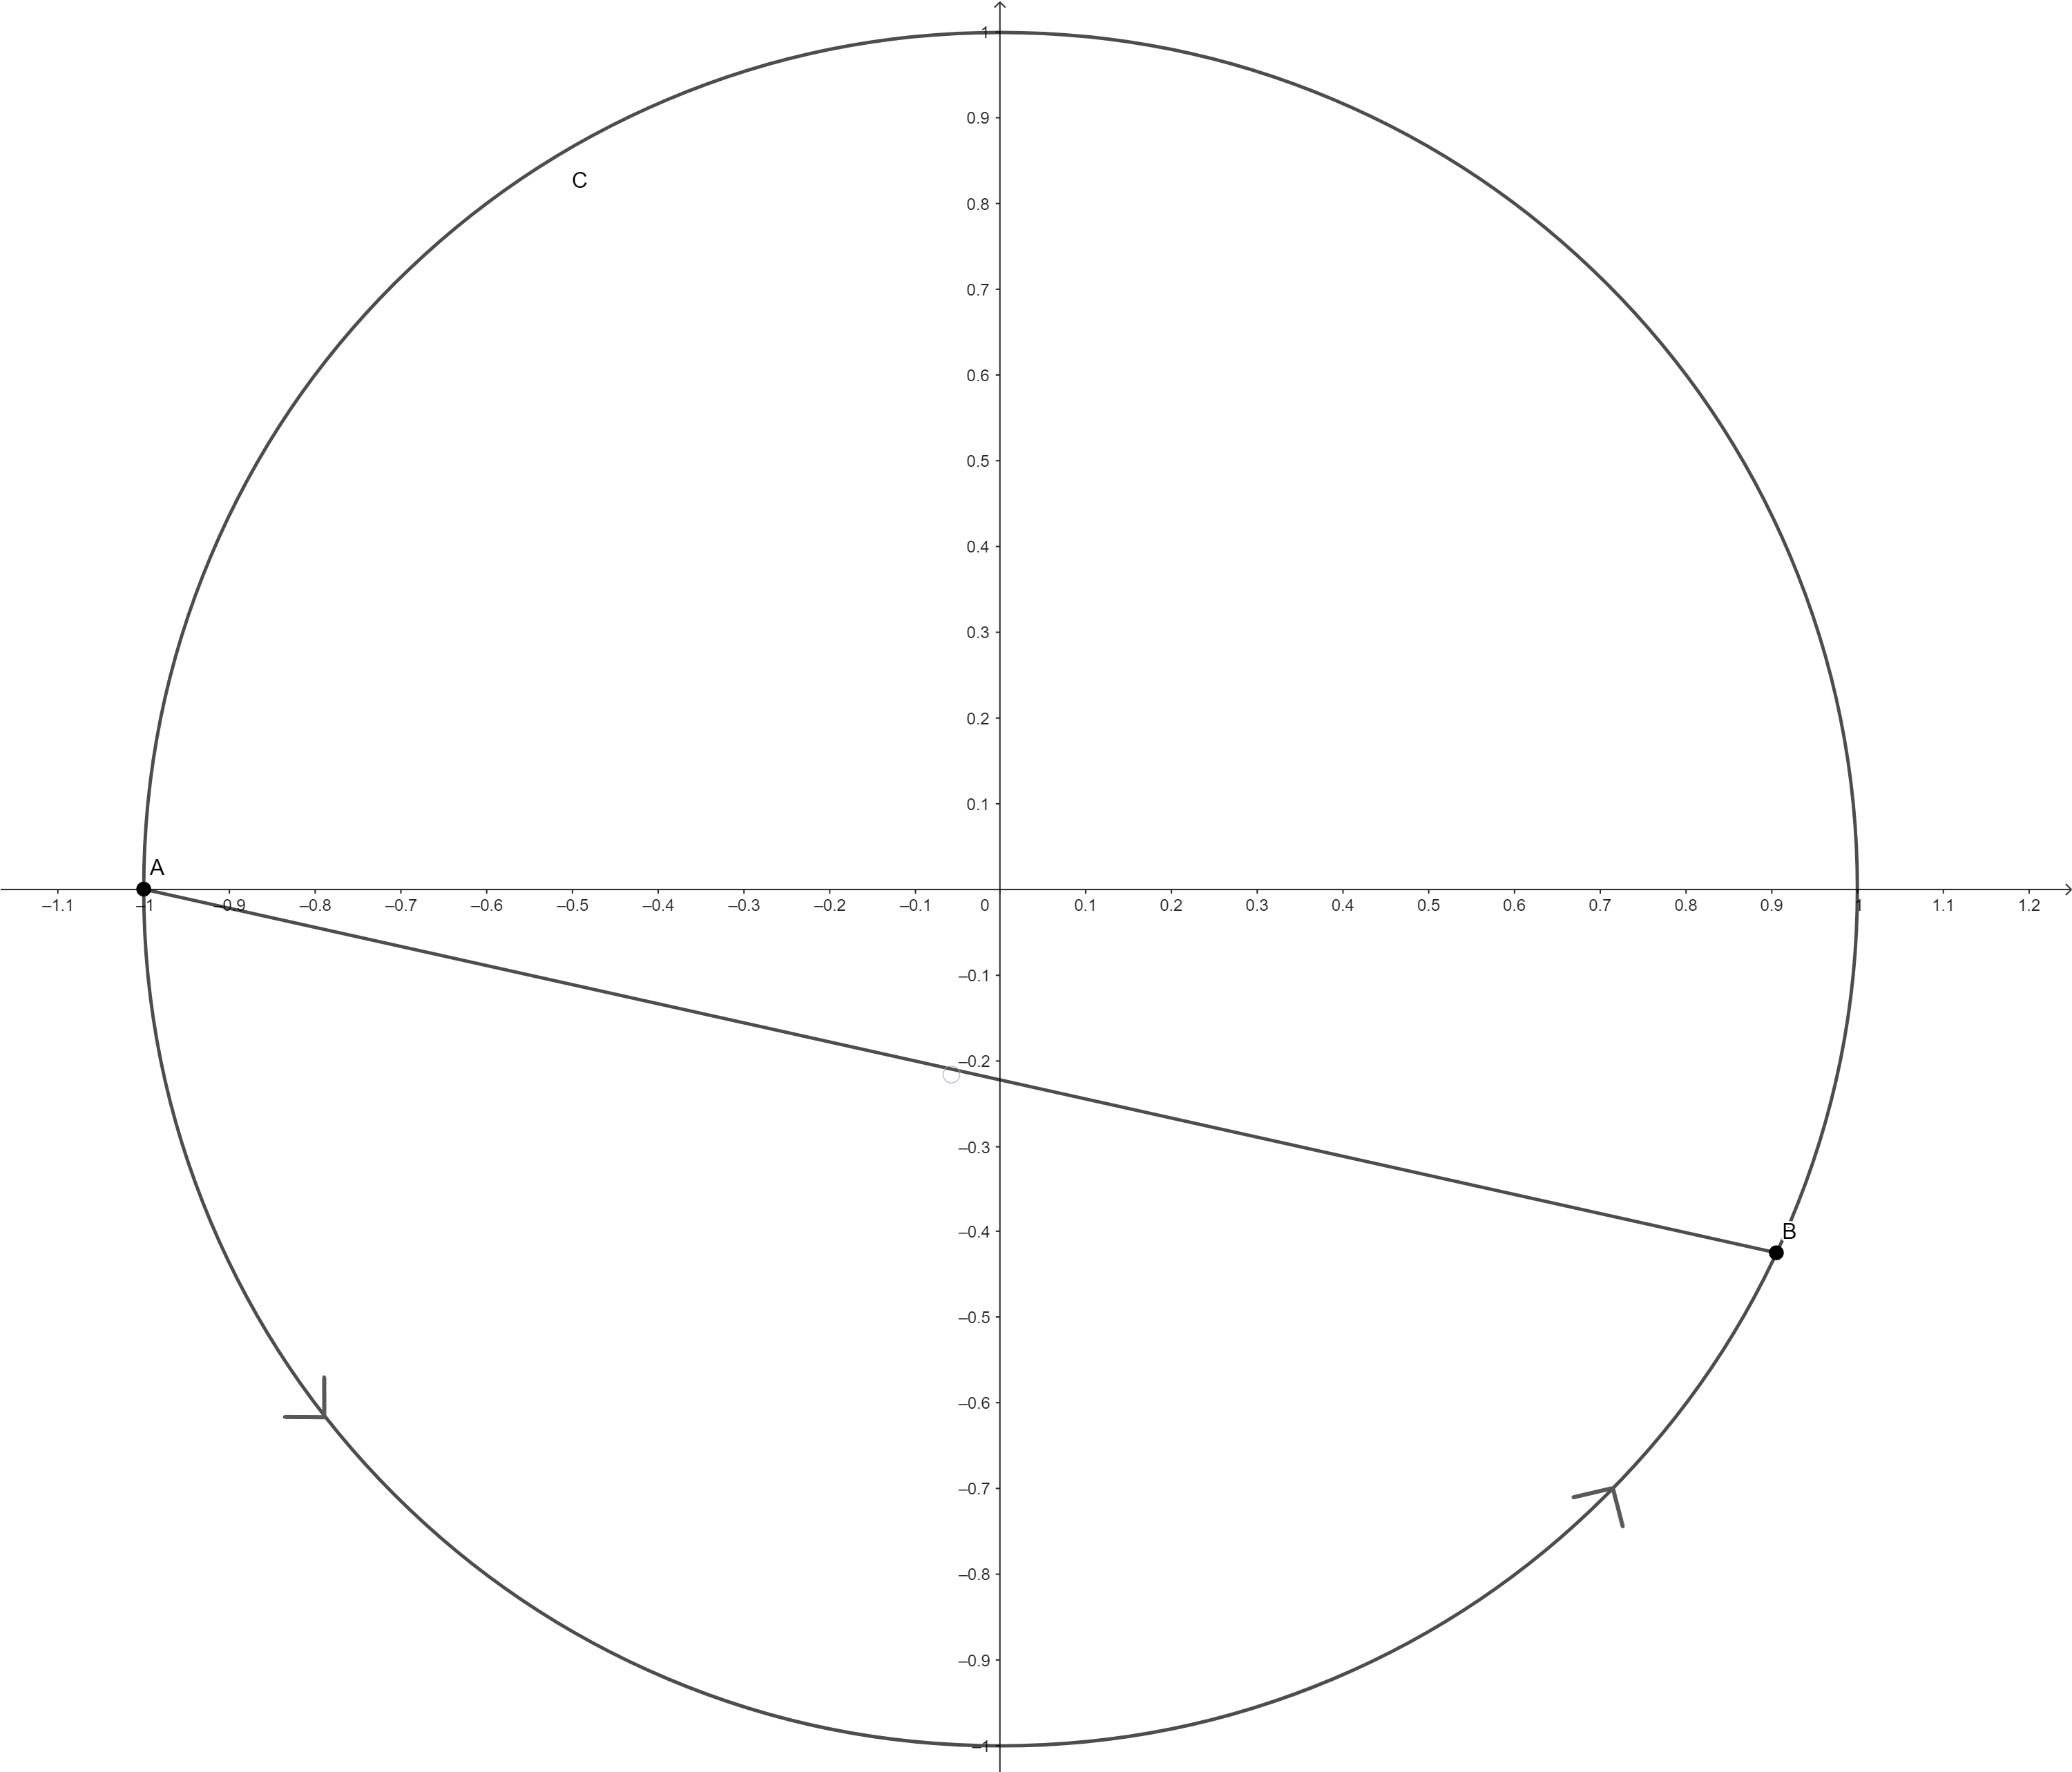
\includegraphics[scale=0.079]{images/ab_circle2.png}
    \caption{L'image de droite représente un trajet long avec $d_{abs}=1.95$, tandis que la figure de gauche représente un trajet moins long avec $d_{abs}=1.95$.}
  \end{figure}

  On comprend donc qu'avec la possibilité de choisir l'orientation initiale, on peut toujours s'arranger pour former un demi-cercle trigonométrique amenant l'électron de $A$ vers $B$. En considérant ce demi-cercle, on remarque bien que le trajet
  amenant le plus loin est à la moitié de sa circonférence, soit $\pi$, et qu'il n'est pas nécessaire de laisser l'électron progresser au delà. On considère donc l'appui du bouton à un tel emplacement.

  \begin{figure}[H]
    \centering
    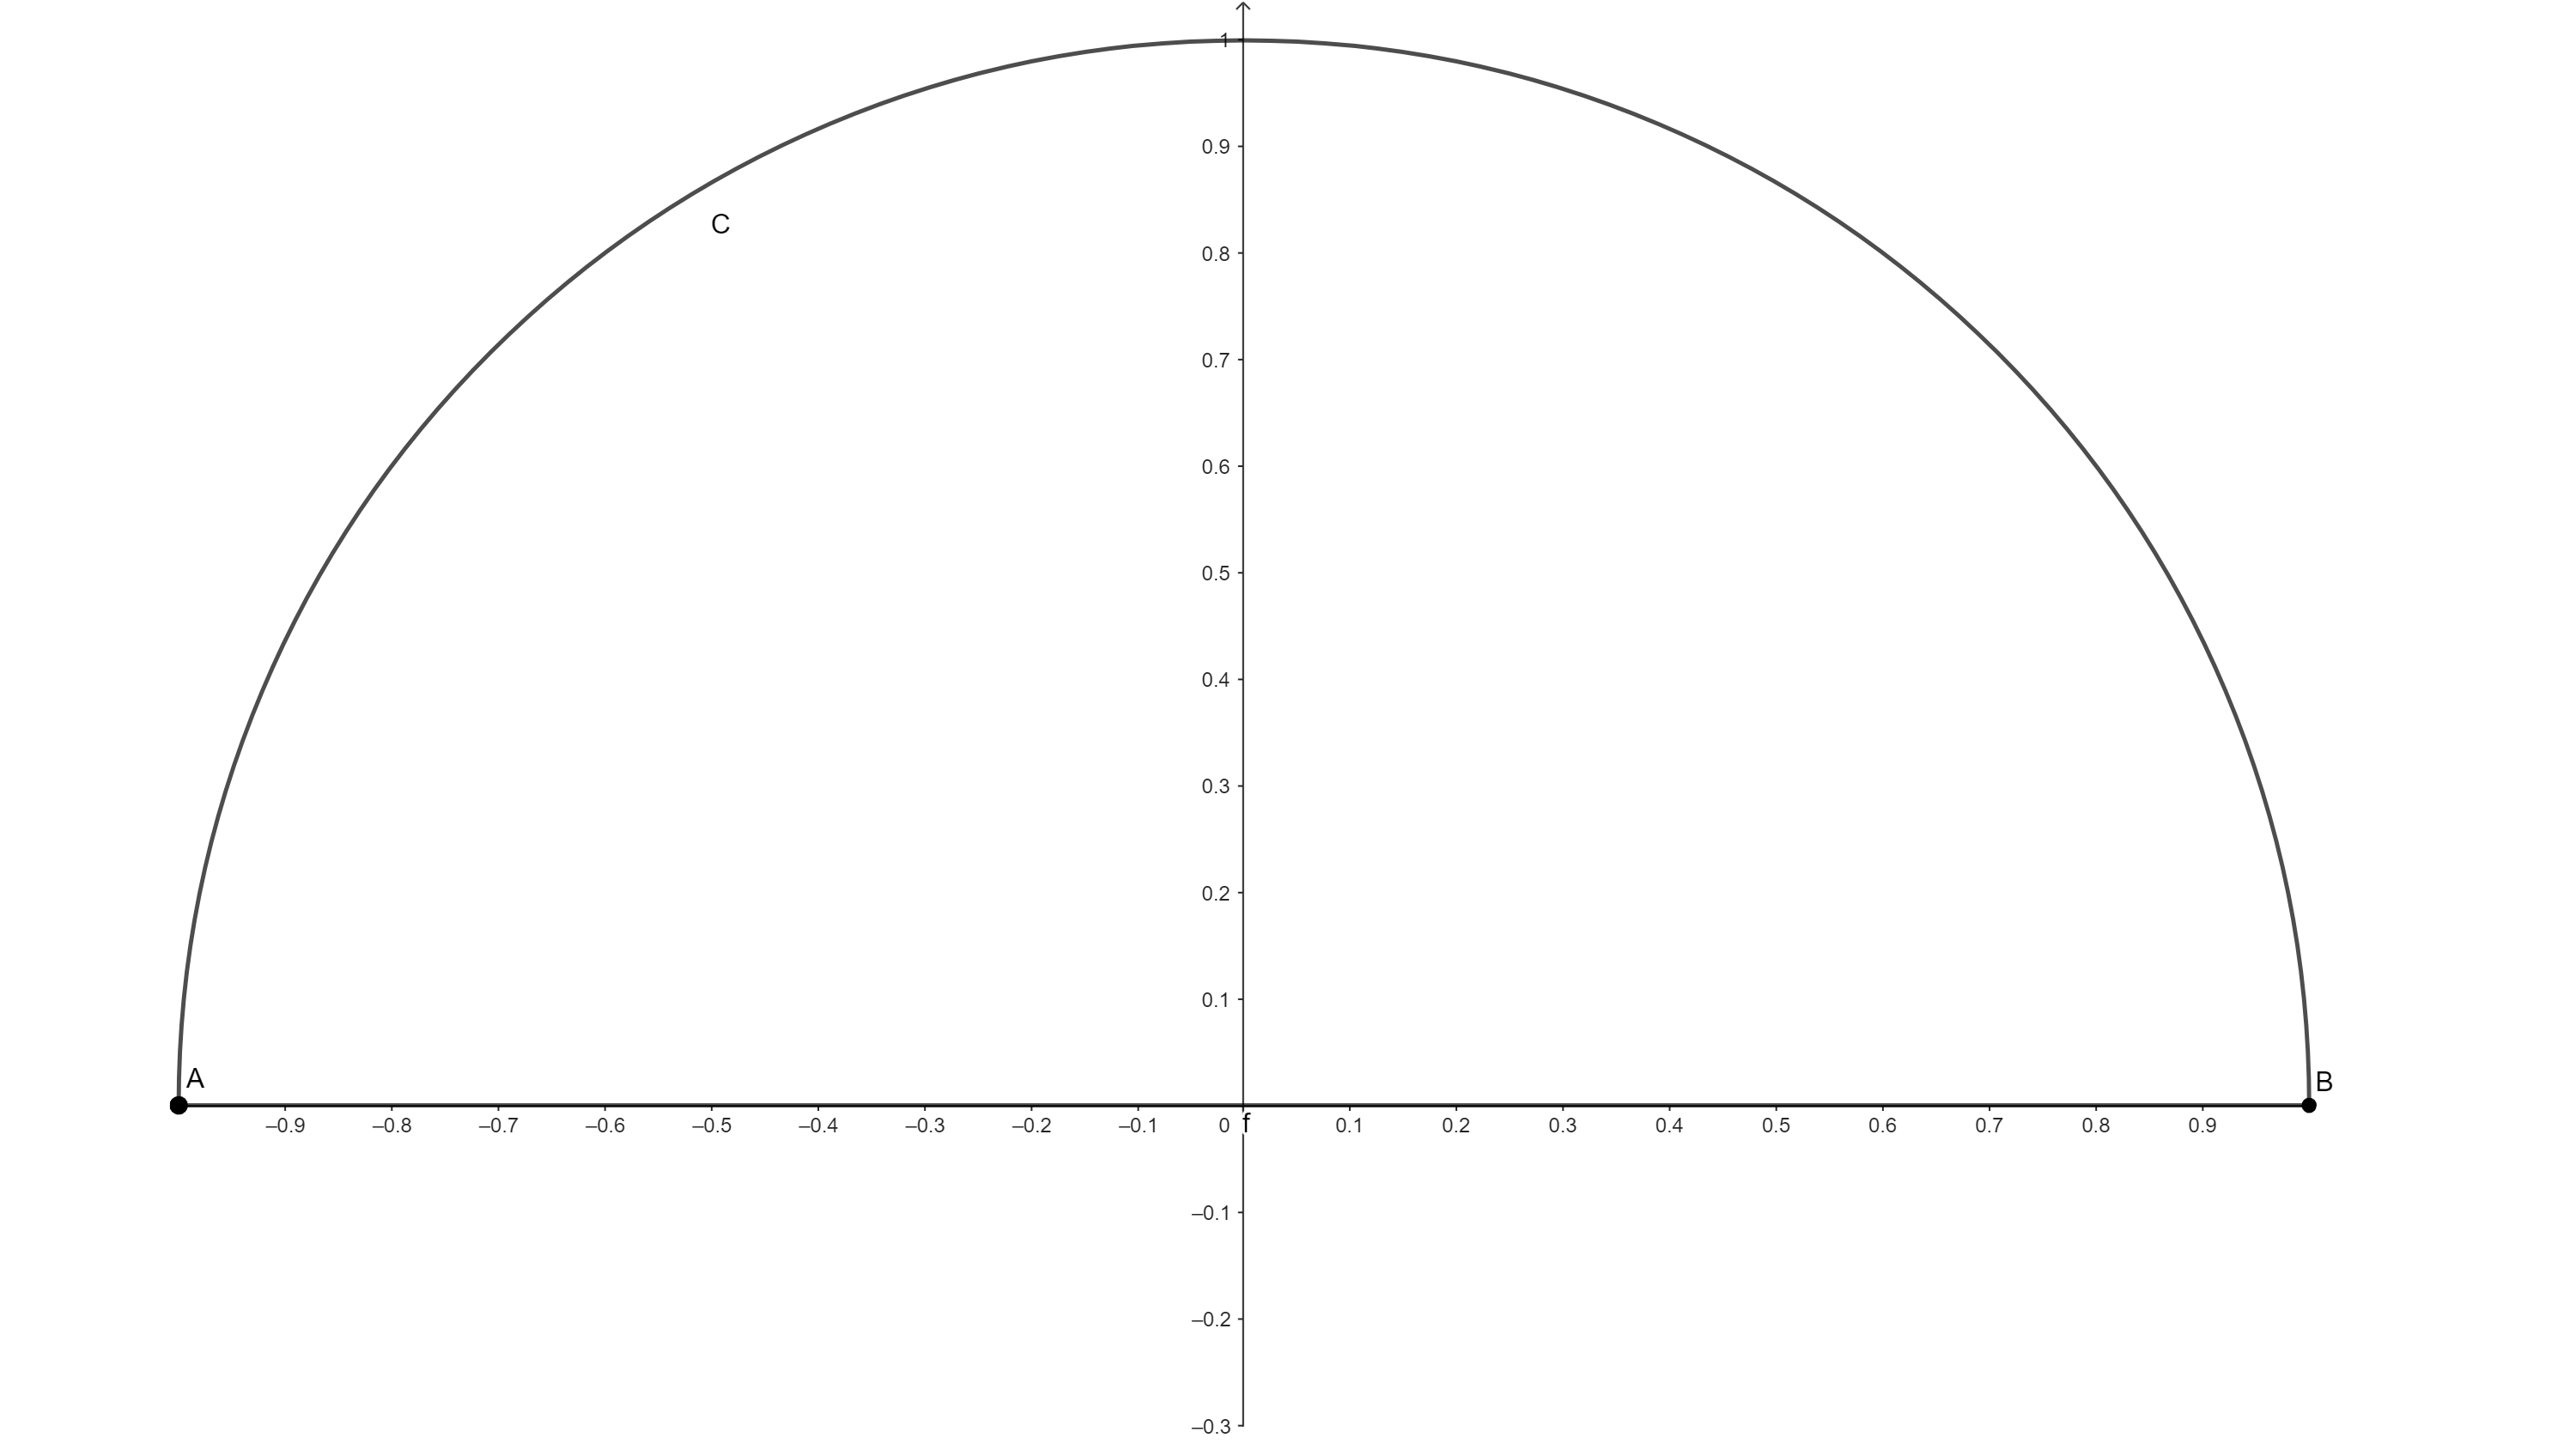
\includegraphics[scale=0.1]{images/ab_circle.png}
    \caption{Un trajet pratique avec $d_{abs}=2$, le diamètre étant le maximum.}
  \end{figure}

\end{proof}

\begin{theorem}
  Soit A,B deux points dans un plan orthonormé. Avec un trajet formant un demi-cercle perpétuel de $A$ à $B$ et la possibilité de changer de direction à des points $C_0, C_1$, ... $C_{n-1}, C_{n}$ (selon l'énoncé),$n\in\mathbb{N}$, le trajet le plus court
  est le demi-cercle perpétuel de $A$ à $B$, avec le centre des cercles associés aux points $A,C_0, C_1$, ... $C_{n-1}, C_{n}$ et $B$ alignés.
\end{theorem}

\begin{proof}
  On comprend qu'afin de maximiser la distance minimale entre $A$ et $B$, il faut que la courbe passant par $A$ et $B$ aie une forme se rapprochant d'un droite.
  Le problème réside donc dans la question: Il y a t'il un moyen de conformer les points $A$, $C_0, C_1, ... C_n$ et $B$ afin de faire une courbe se rapprochant d'une droite, voire même, est-il possible que $d_{min}\approx d_{abs}$.\\

  Connaissant, d'après le \textbf{Théorème 3.2}, qu'il faut appuyer idéalement à la moitié de la circonférence, on peut dors-et-déjà déduire le fait que par récurrence, appuyer perpétuellement à la moitié de la circonférence amènera l'électron le plus loin
  possible (soit donc former des demi-cercles perpétuels avec un alignement nécessaire entre les centres des cercles associés au tirs). Mais, nous pouvons affirmer ce principe par une autre justification:\\

  Dans le cas où $n_{bouton}=0$, le \textbf{Théorème 3.1}, démontre la distance $d_{min}$ selon $d_{abs}$ et nous considèrons $d_{min}$ tel un unique demi-cercle trigonométrique.\\

  Dans le cas où $n_{bouton}=1$, avec la figure ci-dessous, nous comprenons bien que la même propriété s'applique avec $d_{abs}=4$ et $d_{min}=2\pi$:

  \begin{figure}[H]
    \centering
    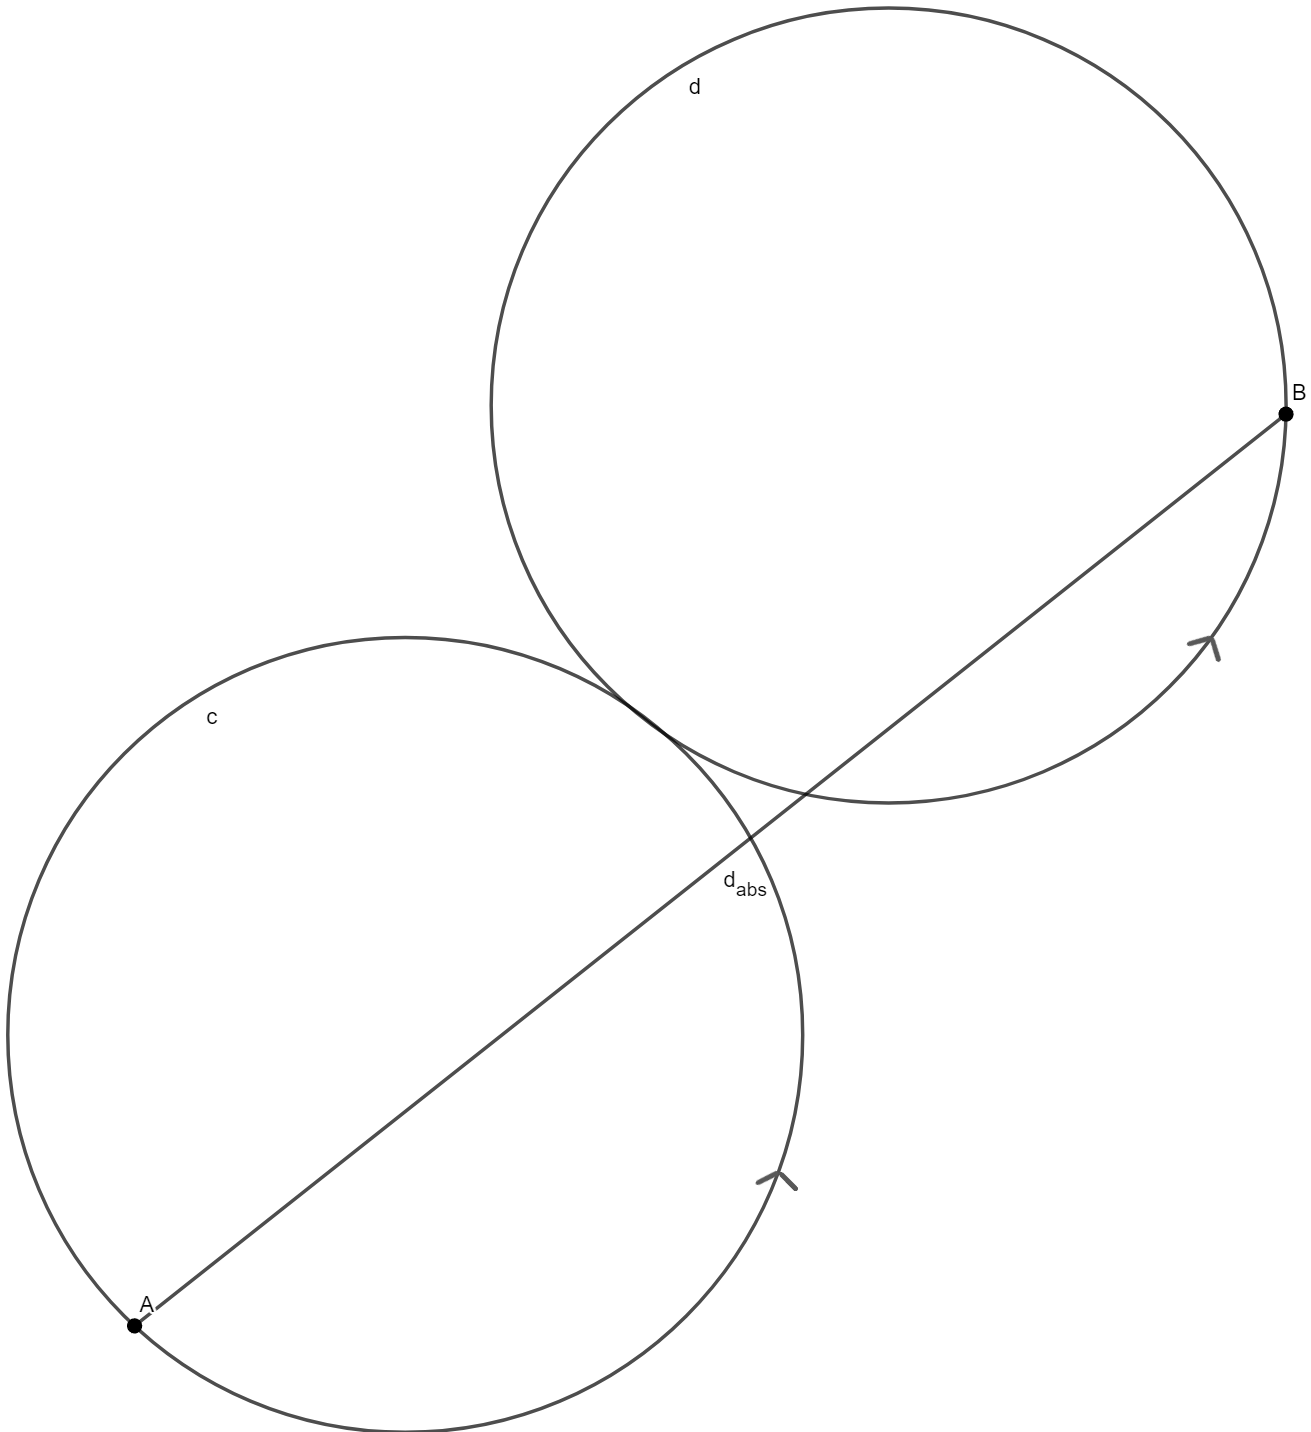
\includegraphics[scale=0.15,valign=t]{images/2_worst.png}
    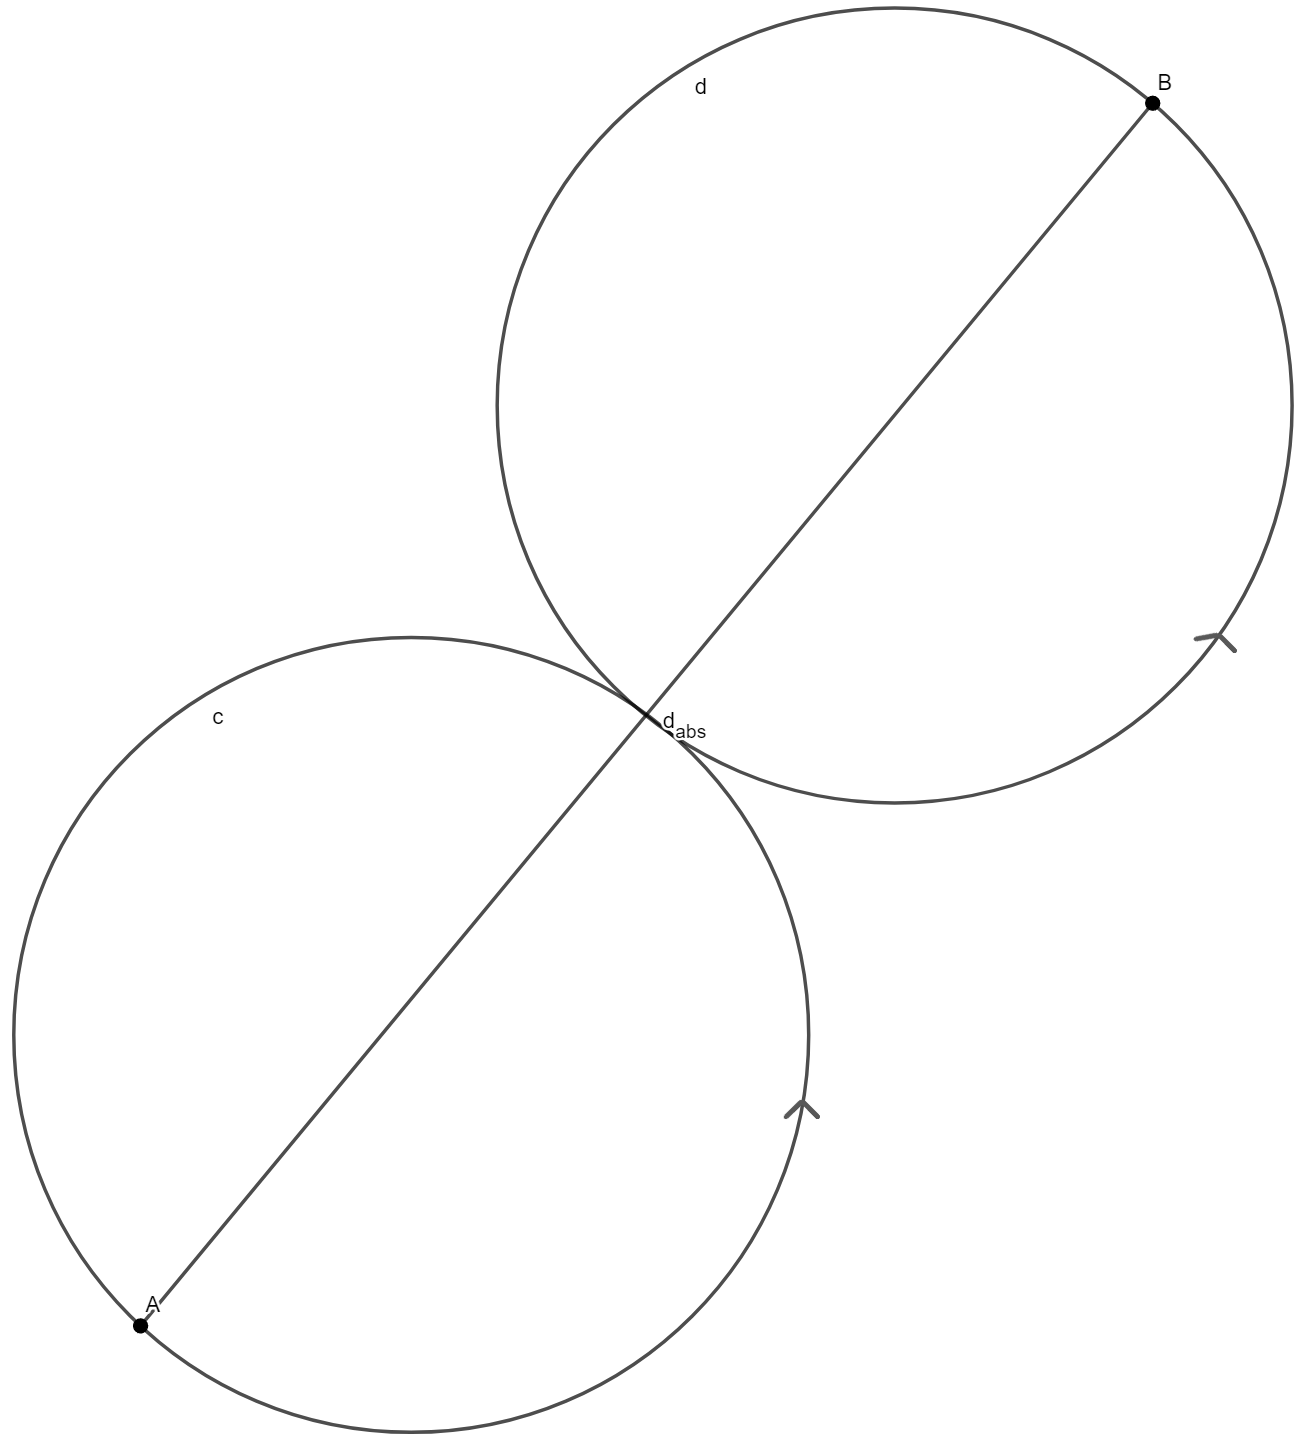
\includegraphics[scale=0.15,valign=t]{images/2.png}
    \caption{La figure de droite est détient $d_{abs}=4$, à son maximum.}
  \end{figure}

  Dans le cas où $n_{bouton}=2$, prenons une version simplifiée du problème. On définit un repère orthonormé $(A;I;J)$ tel que \overrightarrow{AJ} $\perp$ \overrightarrow{AB}. On considère donc les points $A(x_A=0,y_A=0)$ et $B(x_B,y_B=0)$ ainsi que les points $C$ et $D$, l'emplacement de l'électron lorsque le bouton a été appuyé.

  Soit le cercle trigonométrique $Z^\prime$ de centre $Z(0;1)$ passant par $A$, le cercle trigonométrique $X^\prime$ de centre $X$ passant par $C$, et le cercle trigonométrique $Y^\prime$ de centre $Y(x_B;1)$ passant par $B$.

  On remarque que $d_{abs}=x_B-x_A=x_B$ et la distance $d_{ZY}=x_Y-x_Z=x_B$ entre les points $Z$ et $Y$, soit $d_{abs}=d_{ZY}$.

  Le cercle trigonométrique ayant un rayon $r=1$, on sait que $d_{abs ZX}=d_{abs XY}=2$. On définit le triangle isocèle $ZXY$, isocèle en $X$ et $\theta$, l'angle de $\widehat{XZY}$ et $\widehat{ZYX}$. Voici une illustration du repère et des objets géométriques:

  \begin{figure}[H]
    \centering
    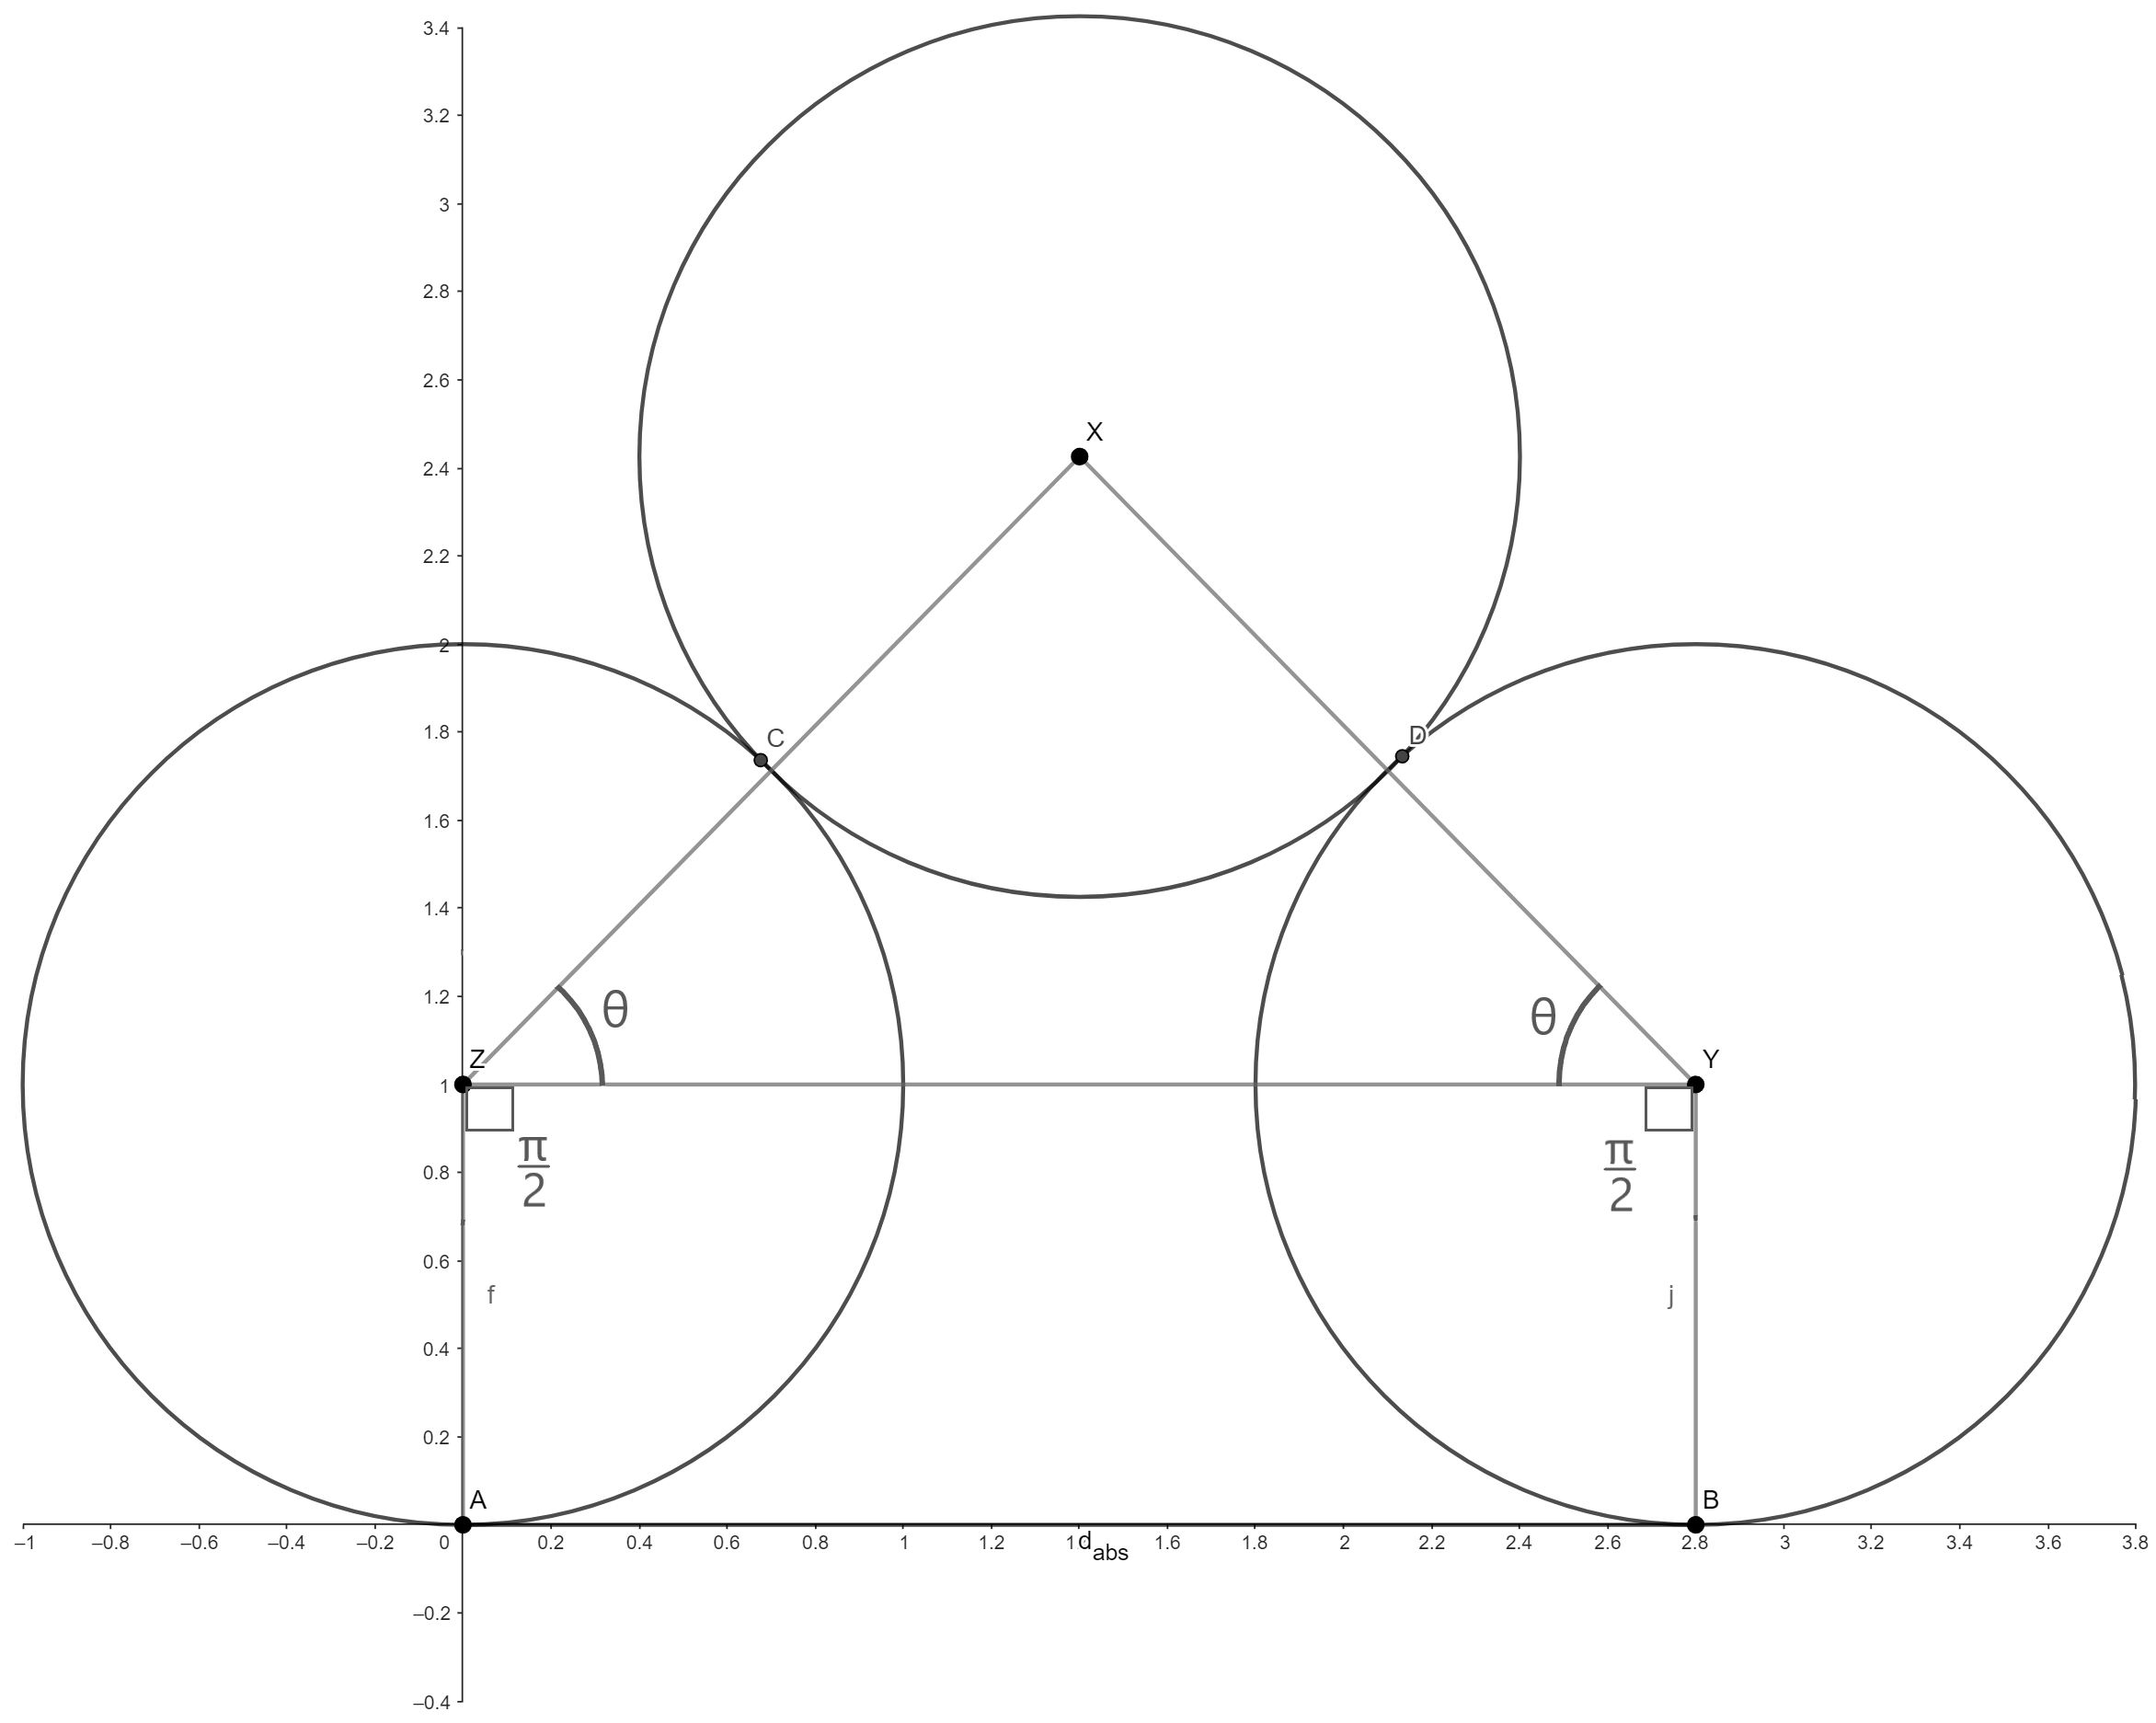
\includegraphics[scale=0.2]{images/three_circles.png}
    \caption{Représentation du repère avec les objets géométriques énoncés.}
  \end{figure}

  La somme des angles d'un triangle équivalent à $\pi$, on sait que $\widehat{ZXY}=\pi-2\theta$.

  D'après le Théorème d'Al-Kashi, nous savons que:

  \[{d_{abs ZY}}^2=ZX^2+XY^2-2ZX\times YX\times cos(\pi-2\theta) \Leftrightarrow {d_{abs ZY}}^2=8+8cos(2\theta)\]

  Avec simplification, nous avons donc:

  \[d_{abs}={d_{abs ZY}}=2\sqrt{2}\sqrt{cos(2\theta)+1}\]

  (On ne considère pas la racine négative de $d_{abs}$ étant donné qu'une longueur est toujours positive).

  Si l'on définit une fonction $f:\mathbb{R^+}\longrightarrow \mathbb{R^+}, x\longmapsto f(x)$ avec $x=\theta$ et $d_{abs}=f(x)$, nous aurons:

  \[f(x)=2\sqrt{2}\sqrt{cos(2x)+1}\]

  On admet que cette fonction admet un maximum en $x=0$ dans l'intervalle $I=[0;\pi[$, avec $f(x)=4$. En d'autres termes, la distance absolue $d_{abs}$ la plus grande possible est égale à 4, avec $\theta=0$. Géométriquement, cela nous la représentation suivante:

  \begin{figure}[H]
    \centering
    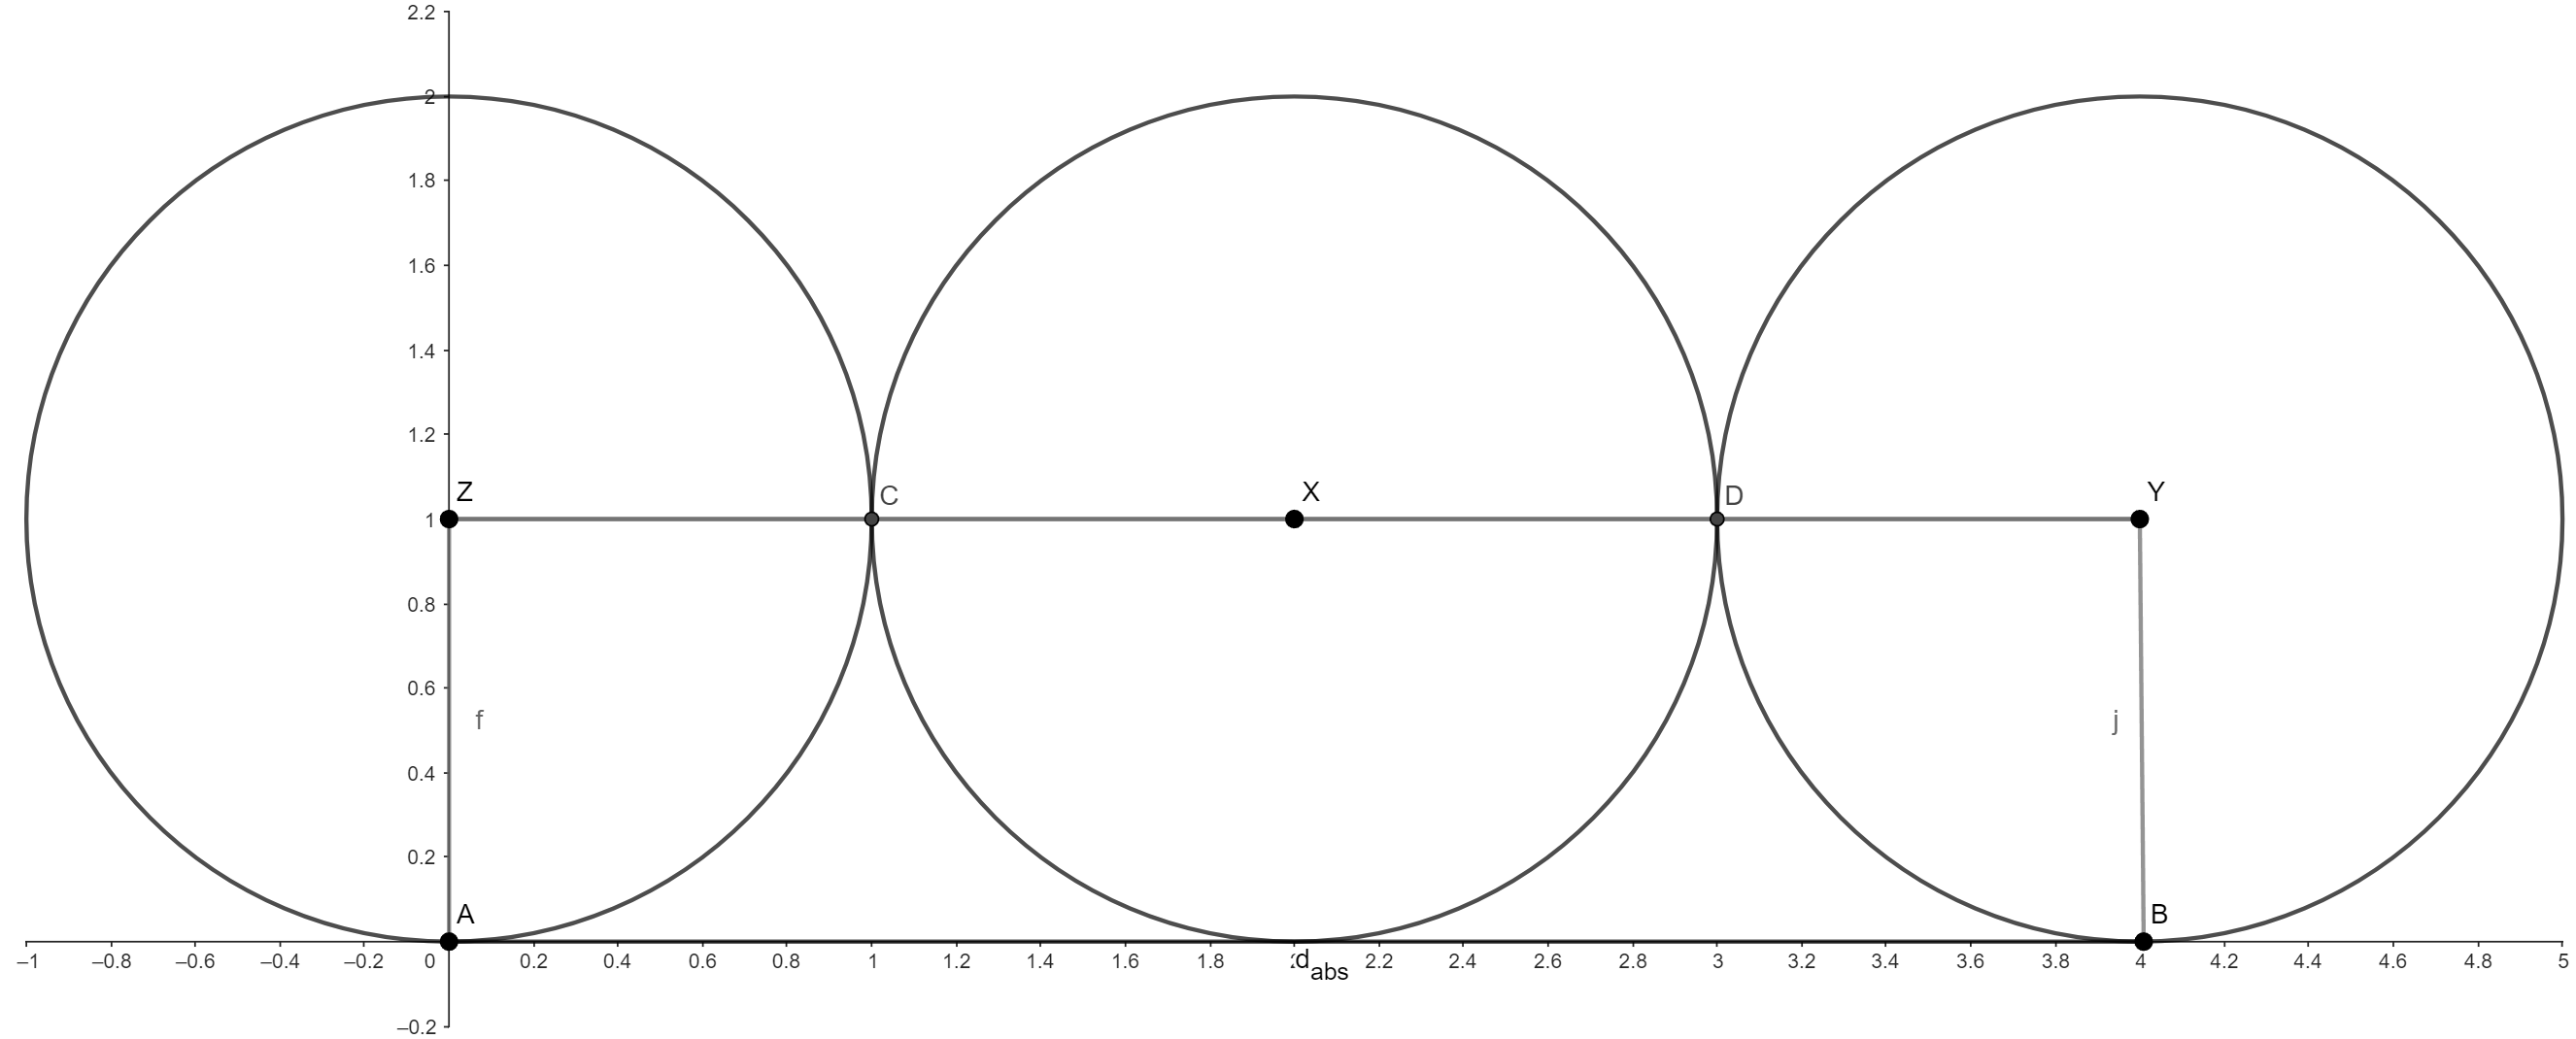
\includegraphics[scale=0.18]{images/perfect_run.png}
    \caption{Représentation du repère avec $d_{abs}=4$.}
  \end{figure}

  On reconnait donc des demi-cercles perpétuels. Si l'on mesure la longueur du trajet de l'électron, nous avons bien $d_{min}=\frac{\pi}{2}+\pi+\frac{\pi}{2}=2\pi$ (résultat notamment en accord avec la réponse à la question 1.a. À noter aussi que la Figure 10 et la Figure 12 illustrent aussi le principe d'un même trajet avec un nombre d'appuis différent).

  Si l'on souhaite aussi avoir un trajet maximal avec le même nombre d'appuis ($n_{bouton}=2$), on préfèrera considérer le point $A$ aux coordonnées $(-1;1)$ et le point $B(6;1)$ avec $d_{abs}=6$ et $d_{min}=3\pi$.

  On considère par la suite des réponses aux questions que $d_{min}$ selon $d_{abs}$ peut-être trouvé à partir de demi-cercles perpétuels.

\end{proof}

\begin{theorem}
  Soit $A,B$ deux points dans un plan quelconque. Il est toujours possible d'atteindre $B$ en partant de $A$ en formant des demi-cercles  perpétuels et en pouvant choisir l'orientation initiale.
\end{theorem}

\begin{proof}
  On considère un point $A$ dans un plan quelconque et $C_a$, le cercle trigonométrique passant par $A$.

  À $n_{bouton}=0$, pouvant choisir l'orientation de base du cercle trigonométrique, on en déduit que l'on peut former un nouveau cercle $C_{a^\prime}$ selon les possibilités d'orientation.  $C_{a^\prime}$ a donc pour rayon $r_{a^\prime}\in\mathbb{R^+}, r_{a^\prime}=2$, étant le
  diamètre du cercle trigonométrique. Cela couvre donc tous les points ayant une distance $d=2$ de $A$, soit donc un disque de surface de $4\pi$.

  Après avoir parcouru un trajet $T=\pi$, d'après le \textbf{Théorème 3.2}, on considère le fait d'appuyer sur le bouton ($n_{bouton}=1$) pour pouvoir progresser dans le plan. Par le même raisonnement que lorsque $n_{bouton}=0$,
  on en déduit que l'on peut former un nouveau cercle $C_{a^{\prime\prime}}$ selon les possibilités d'orientation.  $C_{a^{\prime\prime}}$ a donc pour rayon $r_{a^{\prime\prime}},=2r_{a^\prime}=4$ et un disque de surface de $16\pi$.

  Par récurrence, on déduit que l'on peut toujours former un cercle $C_k$ de rayon $r_k=2(n_{bouton}+1)$ impliquant que lorsque $n_{bouton}\to+\infty$, $r_k\to+\infty \implies {\pi}r_k^2\to+\infty$, couvrant ainsi l'ensemble du plan.

  On comprend donc qu'il est possible à partir du point $A$ d'atteindre n'importe quel point $B$ dans le plan.


  Voici une représentation visuelle permettant d'expliquer le raisonnement:
  \begin{figure}[H]
    \centering
    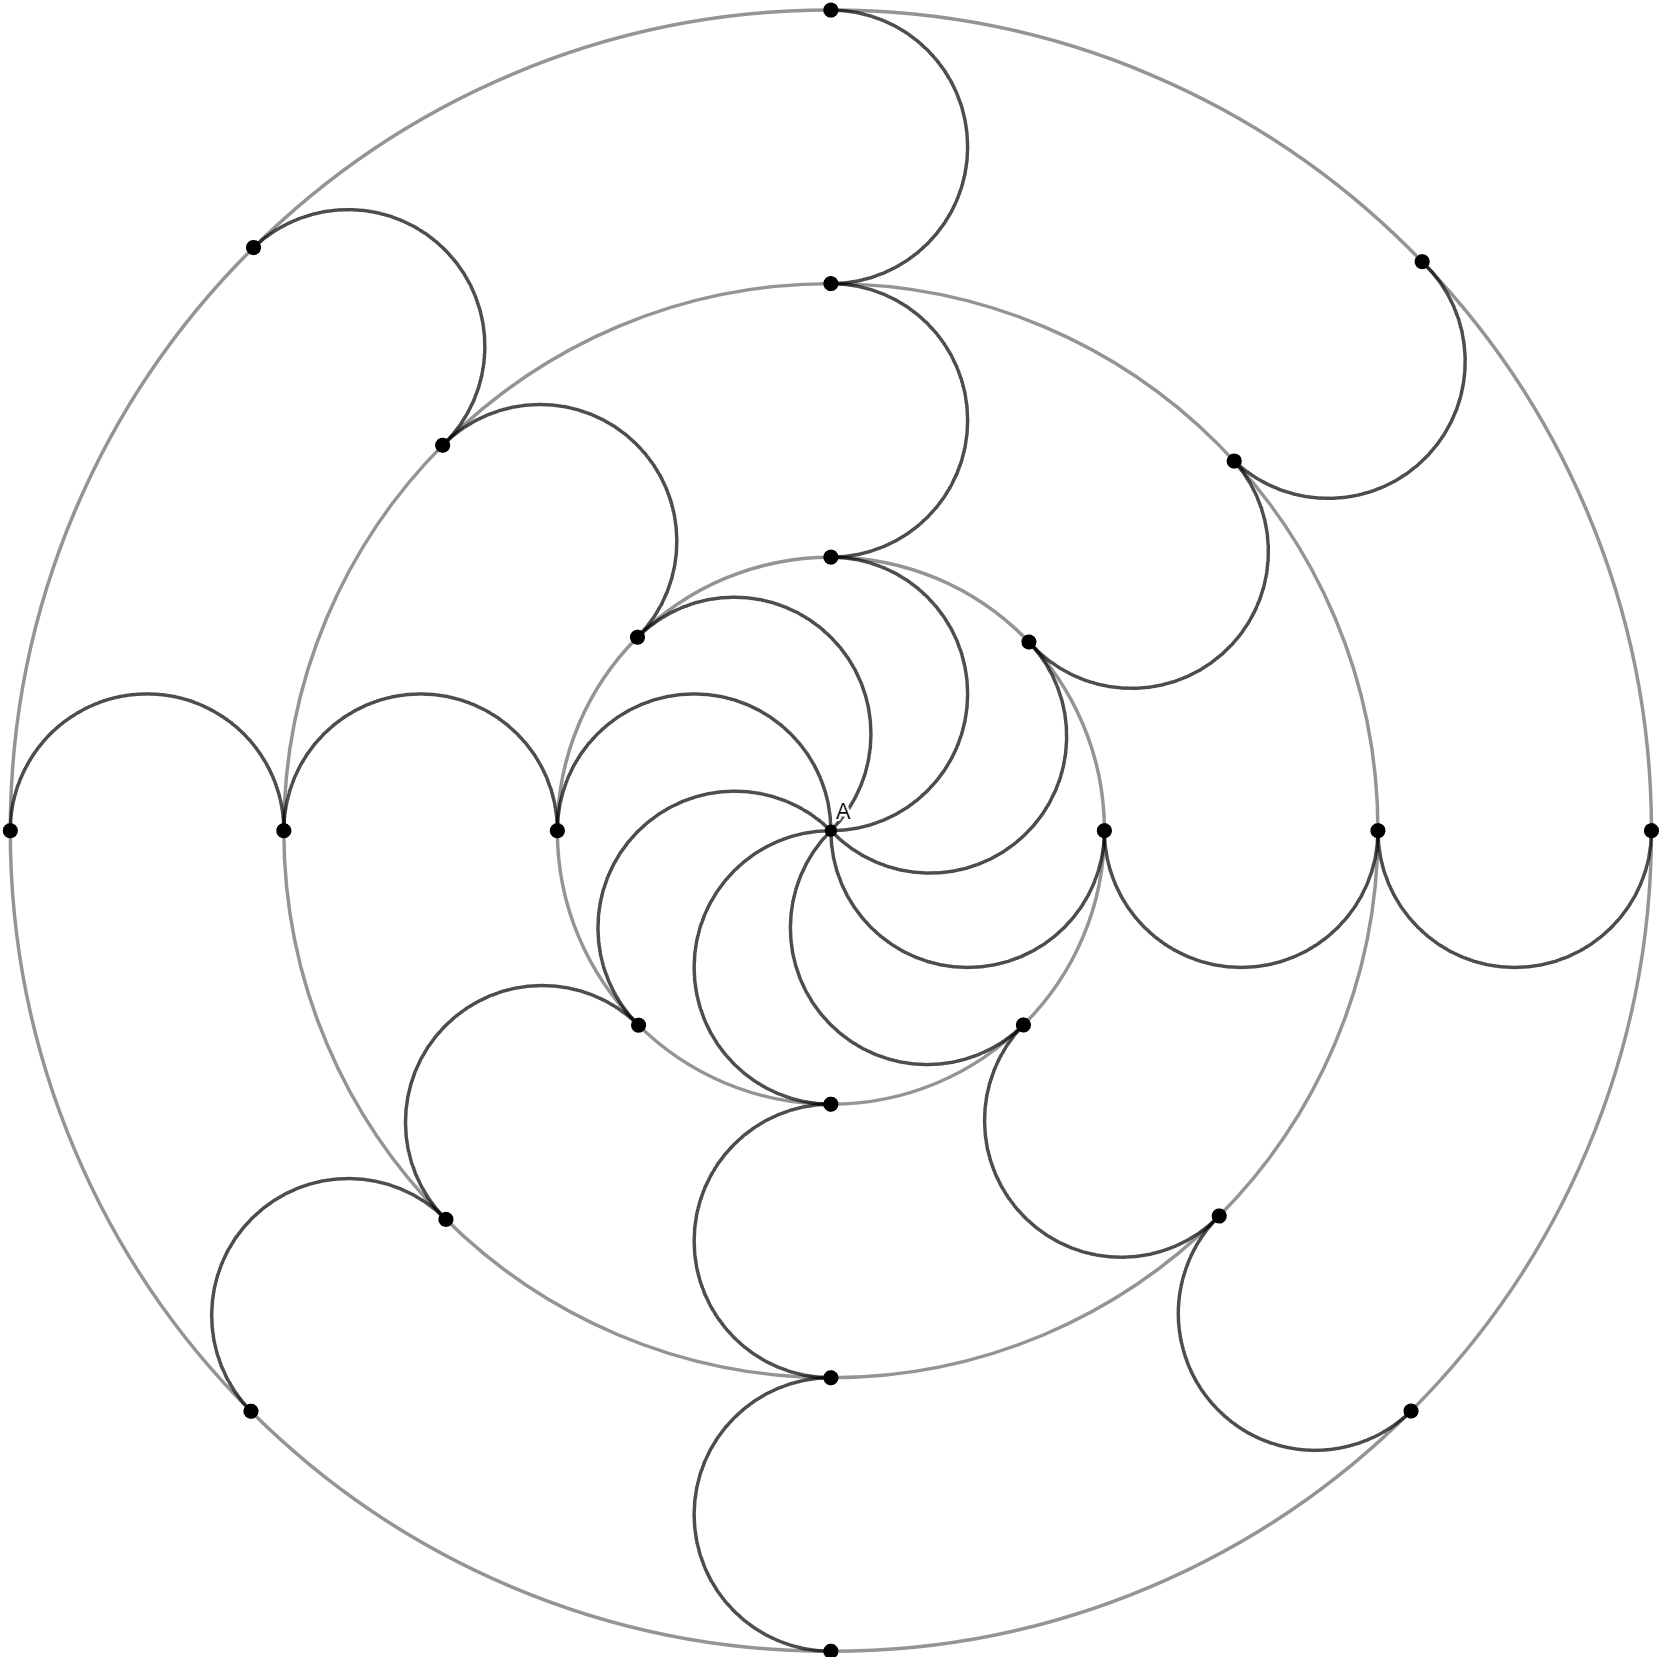
\includegraphics[scale=0.27]{images/visualization.png}
    \caption{Représentations des moyens d'atteindre $B$ en partant de $A$ avec une division=8 selon l'orientation (les points des courbes circulaires ont donc un angle de 45° entre eux selon le point $A$) avec $n_{bouton}=2$.
      Les points noirs sont des points $B$ avec la longueur du segment [AB] un multiple de $2$.}
  \end{figure}
\end{proof}

\section{Réponse à la Question 1}

\textbf{Réponse 1.a}: Comme l'explique le \textbf{Théorème 3.4}, il est toujours possible d'atteindre un point $B$ à partir d'un point $A$ avec des demi-cercles perpétuels, impliquant que Nicolas peut toujours guider l'électron du point $A$ au point $B$.

À partir du même théorème, du \textbf{Théorème 3.2}, ainsi qu'à l'aide de la Figure 13, on remarque que Nicolas doit appuyer lorsque le trajet $d_{abs}=2$, soit donc, lorsque $d_{abs}$ est un multiple de 2, $n_{bouton}\longmapsto n_{bouton}+1$ (lorsque $d_{abs}\leq2, n_{bouton}=0$, lorsque $d_{abs}\in]2,4], n_{bouton}=1$, lorsque $d_{abs}\in]4,6], n_{bouton}=2$, etc...

On peut donc définir $d_{abs}$ tel que $d_{abs}=2(n_{bouton}+1)$, en considérant $d_{abs}$ en tant que la longueur maximale $\in\mathbb{N}$.

Si l'on effectue le raisonnement inverse en cherchant $n_{bouton}$ en fonction de $d_{abs}$, on trouve que $n_{bouton}=\frac{d_{abs}}{2}-1$. Or $d_{abs}\in\mathbb{R^+}$, on s'arrange donc afin de prendre la plus petite valeur entière selon $d_{abs}$

On trouve que :
\[n_{bouton}=\lceil \frac{d_{abs}-1}{2} \rceil\]

Il doit donc appuyer au minimum sur le bouton à $\lceil \frac{d_{abs}-1}{2} \rceil$ de la distance $AB$.\\

\textbf{Réponse 1.b}: On considère les points $A$ et $B$ dans un plan quelconque et $d_{abs}=AB$ (par définition). Comme nous l'avons affirmé précédement avec le \textbf{Théorème 3.3}, nous considérons la formation de demi-cercles perpétuels comme le trajet amenant l'électron le plus loin avec la distance minimale la plus courte possible. Il ne nous reste plus qu'à s'arranger pour former des demi-cercles perpétuels optimisés selon la distance $d_{abs}$ avec l'orientation du canon de manière optimale.

Soit le point $D$ et $C$ tel que $DC=1$ et $CB=1$ (en d'autres termes, $C$ est le centre du cercle trigonométrique passant par $D$ et $B$) avec $A,D,C$ alignés.

On définit aussi le point $D$ tel qu'il soit le nombre de demi-cercles complets possibles à réaliser à partir de la distance absolue $d_{abs}$ en partant du point $A$, soit le plus petit entier naturel étant divisible (et non pas divisé) par le diamètre du cercle trigonométrique selon $d_{abs}$. On le définit donc à partir du point $A$ tel que $AD=2\lceil\frac{d_{abs}}{2}\rceil$. Soit $\alpha$ l'angle $\widehat{DCB}$, égal aussi au trajet circulaire de $D$ à $B$, étant dans un cercle trigonométrique.

Nous aurons donc une représentation semblable à la figure ci-dessous:

\begin{figure}[H]
  \centering
  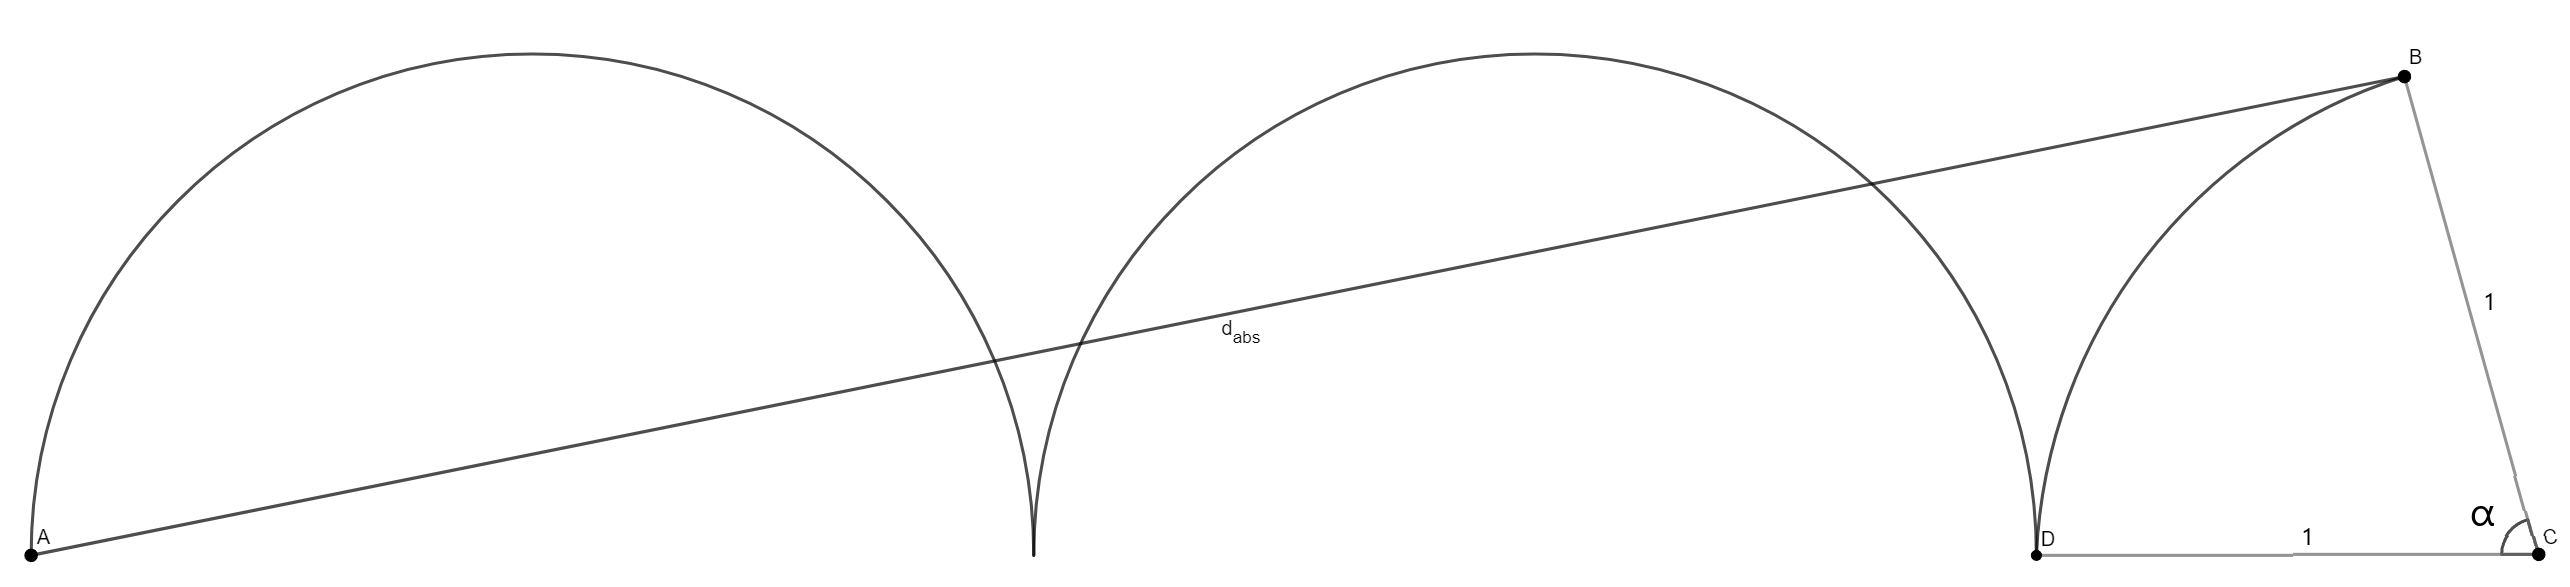
\includegraphics[scale=0.2]{images/dmin.png}
  \caption{Représentation des points A,B,C,D, dans le cas où $n_{bouton}=2$.}
\end{figure}

Nous avons donc $AC=AD+DC=2\lceil\frac{d_{abs}}{2}\rceil+1$.

D'après le Théorème d'Al-Kashi, nous savons que:

\[AB^2=AC^2+BC^2-2\times AC \times BC \times cos(\alpha)\]

Soit:

\[{d_{abs}}^2=(2\lceil\frac{d_{abs}}{2}\rceil+1)^2 +1 -2(2\lceil\frac{d_{abs}}{2}\rceil+1) cos(\alpha)\]

En isolant $\alpha$, nous avons:

\[\alpha=\arccos(\frac{AB^2-AC^2-BC^2}{-2BC\times AC})\]

En d'autres termes,

\[\alpha=\arccos(\frac{{d_{abs}}^2 -(2\lceil\frac{d_{abs}}{2}\rceil+1)^2-1}{-2(2\lceil\frac{d_{abs}}{2}\rceil+1)})=\arccos(\frac{(2\lceil\frac{d_{abs}}{2}\rceil+1)^2+1 -{d_{abs}}^2}{2(2\lceil\frac{d_{abs}}{2}\rceil+1)})\]

$AD$ répresentant la distance absolue du nombre de demi-cercles complets, on sait qu'à chaque diamètre traversé, on y associe un trajet $d_{min}=\pi$ sur le cercle trigonométrique. On définit donc $d_{demi-cercle}=\frac{AD}{2}\pi=\lceil \frac{d_{abs}}{2} \rceil\pi$, avec $d_{demi-cercle}\in\mathbb{R^+}$ désignant la distance parcourue sur les demi-cercles complets formés à partir de $AD$.

$\alpha$ étant aussi le trajet circulaire de $D$ à $B$, on trouve comme distance minimale de l'électron pour aller de $A$ à $B$ en trajet circulaire:

\[d_{min}=d_{demi-cercle}+ \alpha\]

Soit:

\[d_{min}= \lceil\frac{d_{abs}}{2}\rceil\pi + \arccos(\frac{(2\lceil\frac{d_{abs}}{2}\rceil+1)^2+1 -{d_{abs}}^2}{2(2\lceil\frac{d_{abs}}{2}\rceil+1)})\]

Avec $d_{min}$ la distance minimale parcoure par l'électron en fonction de $AB$ ($d_{abs}$).

\section{Théorèmes pour la Question 2}

À partir de la question 2, nous considérons le canon à électrons placé aux abords d'un cercle de rayon $r>0$. L'objectif est que le trajet circulaire de l'électron ne touche pas la bordure du cercle de rayon $r$. Voici une illustration:

\begin{figure}[H]
  \centering
  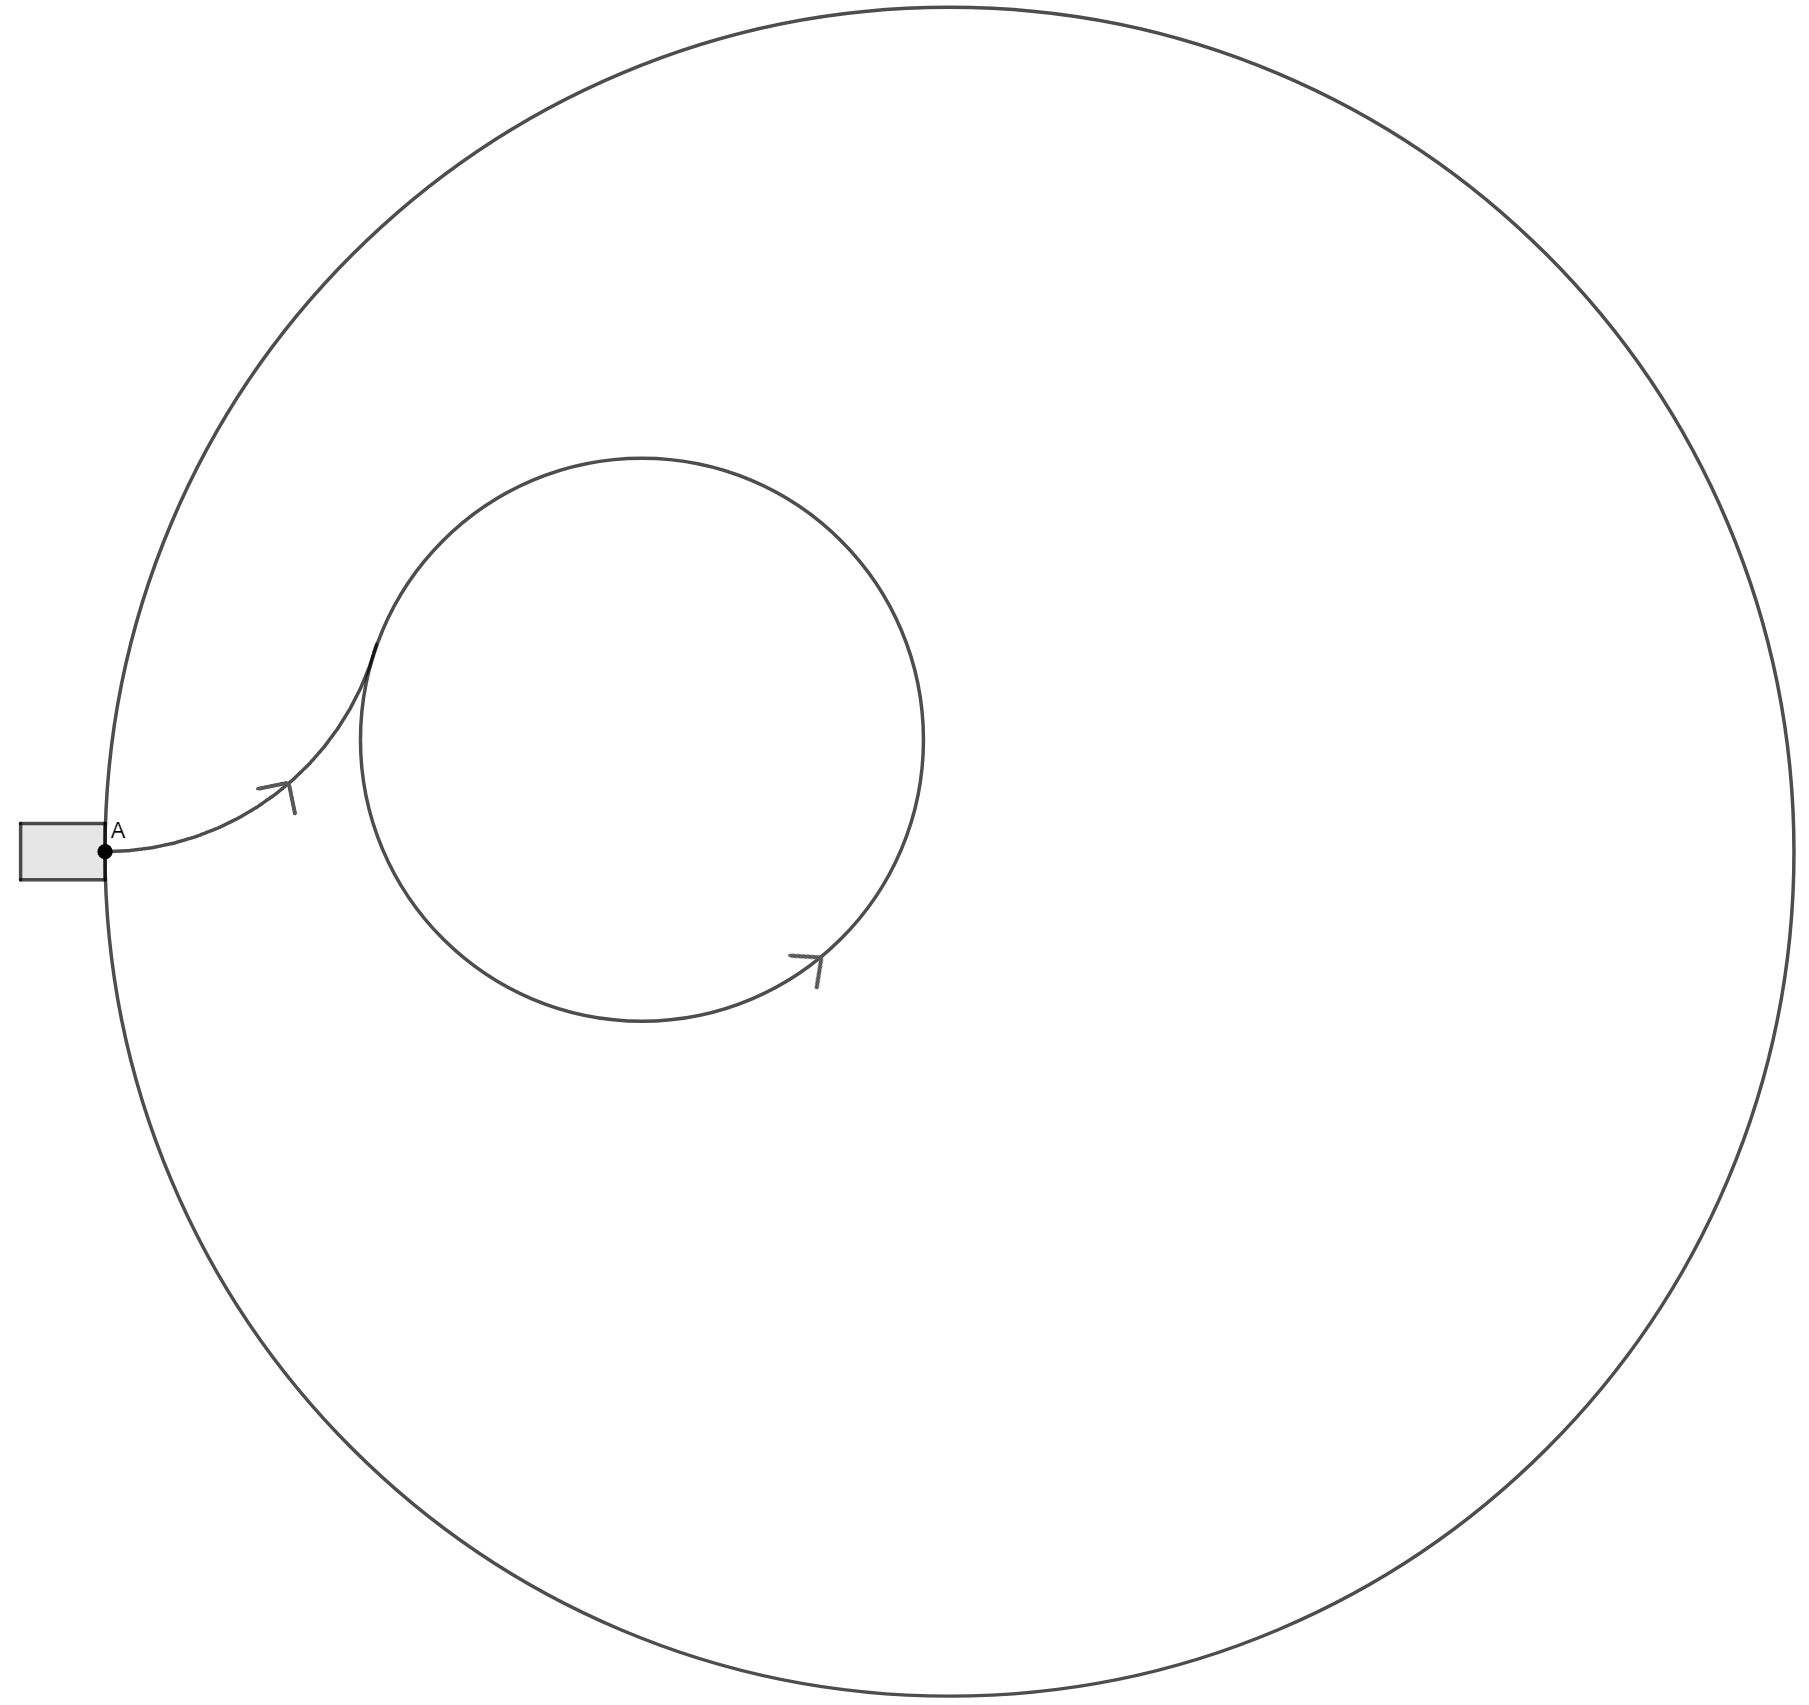
\includegraphics[scale=0.15]{images/inside_circle.png}
  \caption{Un trajet circulaire de l'électron stable avec $r=3$ et $n_{bouton}=1$.}
\end{figure}

\begin{theorem}
  Il faut au minimum appuyer une fois ($n_{bouton}=1$) afin d'éviter que l'électron touche le cercle $C_r$ de rayon $r$.
\end{theorem}

\begin{proof}
  Supposons qu'il soit possible qu'il existe un trajet stable sans appuyer sur le bouton ($n_{bouton}=0$).

  Cela n'est pas possible car, l'électron étant placé au bord du cercle $C_r$ de rayon $r>0$, on sait que le centre du cercle de son trajet est placé en dehors de $C_r$. On en déduit qu'il n'est pas possible
  d'inscrire un trajet stable dans $C_r$.

  \begin{figure}[H]
    \centering
    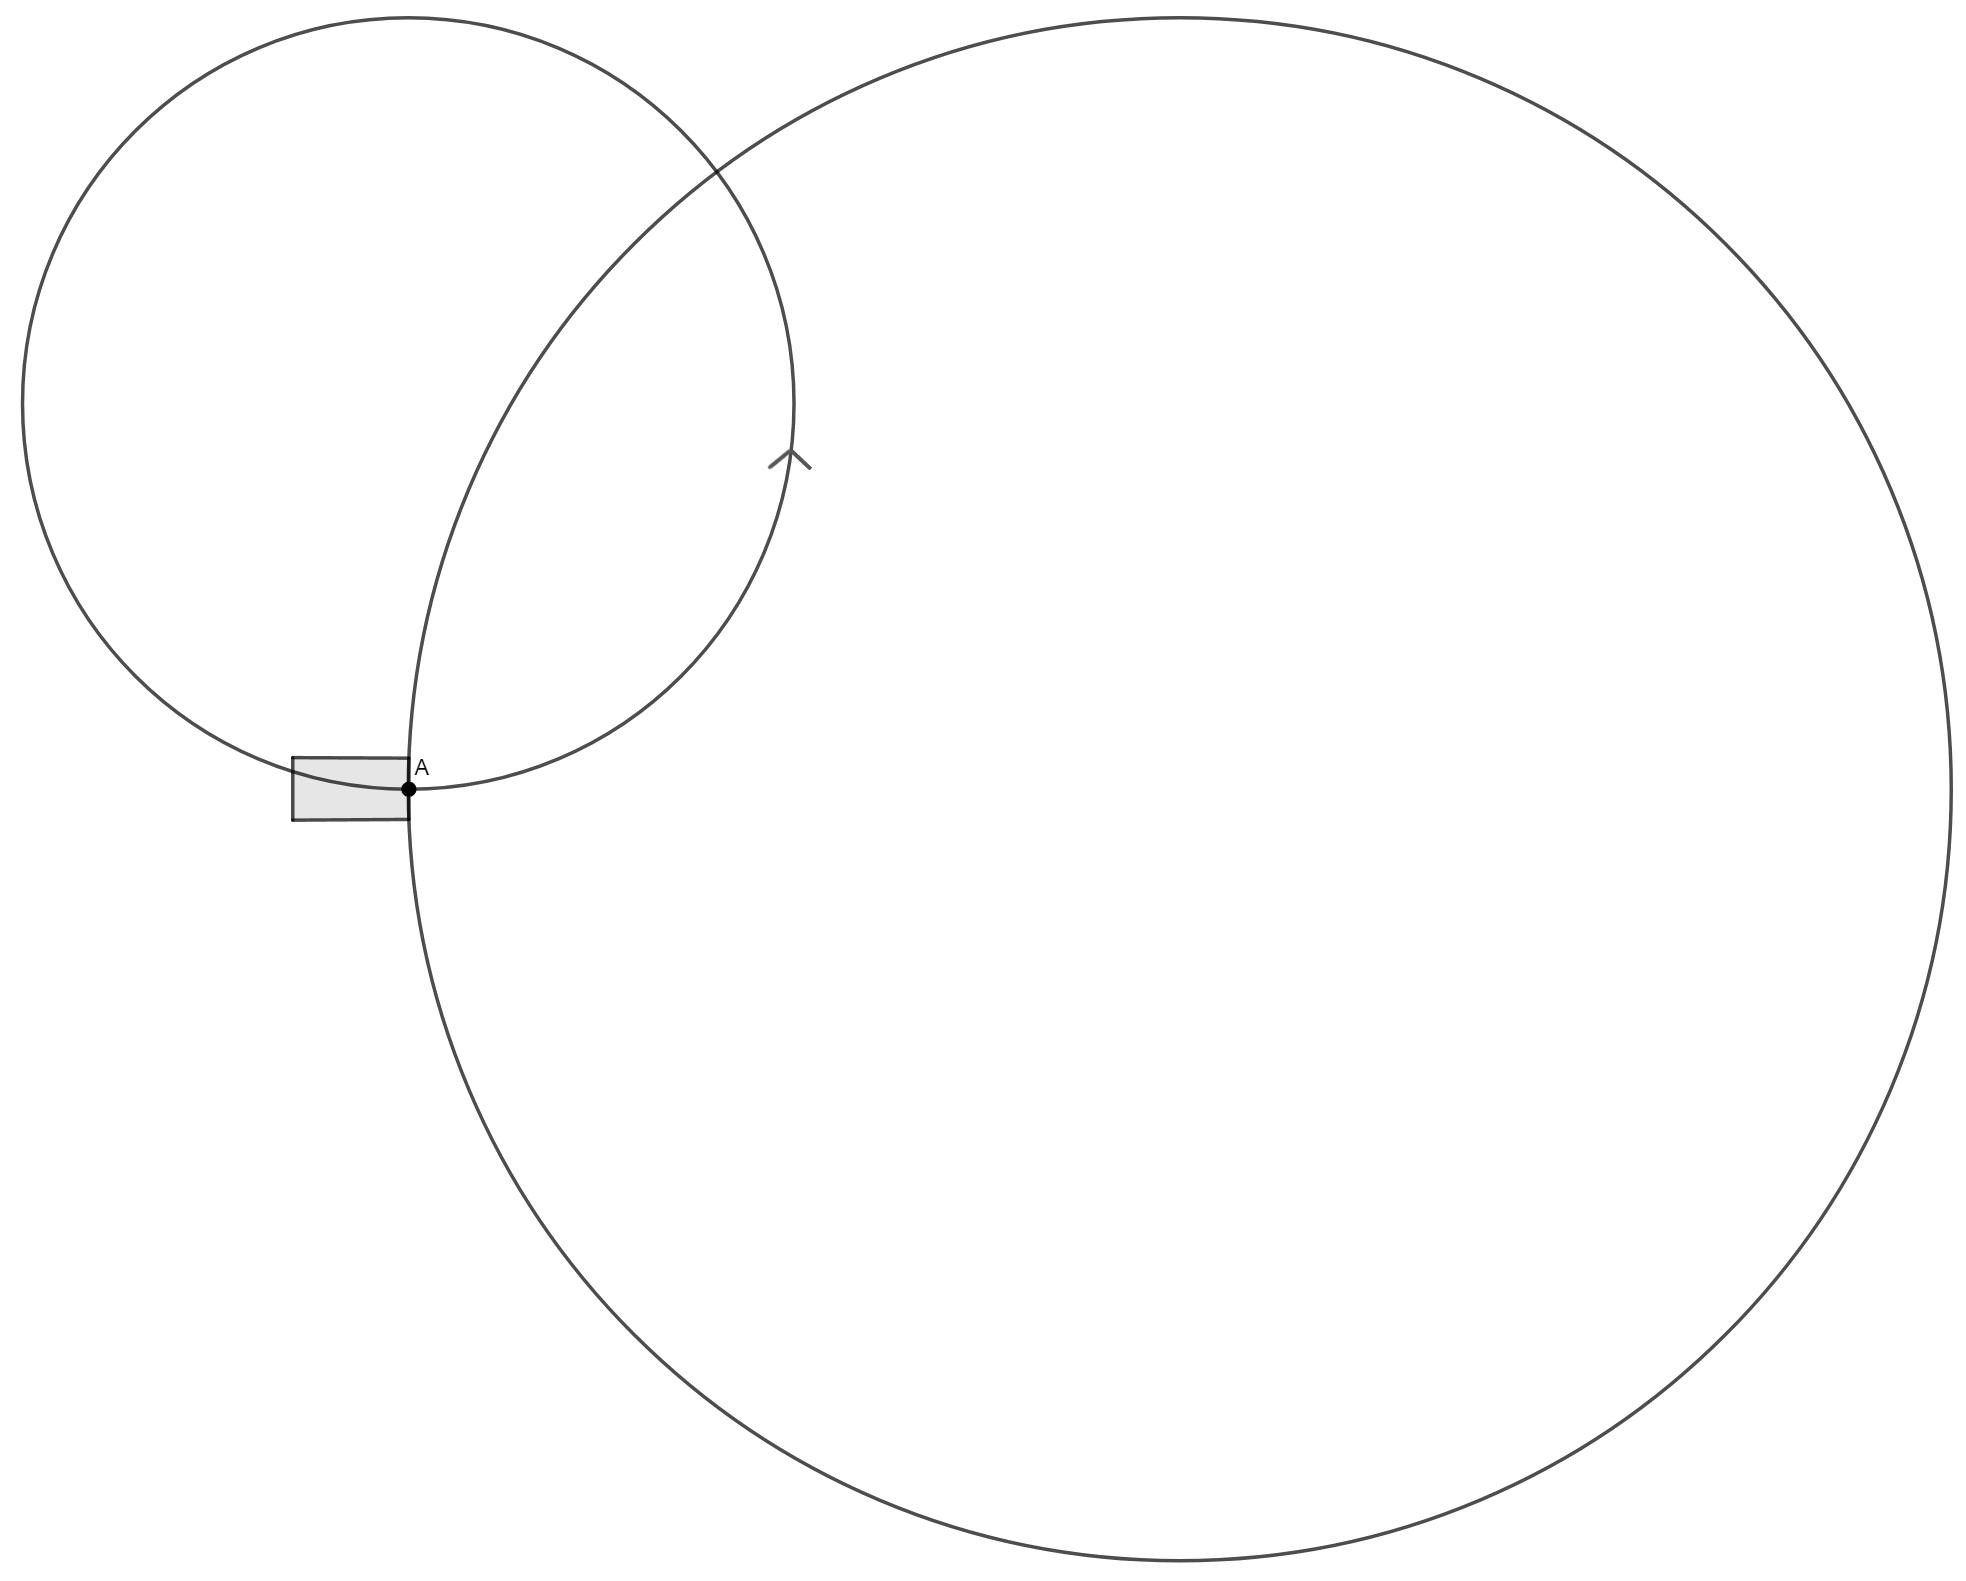
\includegraphics[scale=0.15]{images/not_possible.png}
    \caption{Représentation du trajet lorsque $n_{bouton}=0$ (avec $r=2$).}
  \end{figure}
\end{proof}

\begin{theorem}
  On considère d'appuyer sur le bouton au milieu de la circonférence inscrite dans le cercle $C_r$ de rayon $r>0$ pour trouver le trajet stable avec $r$ à son minimum.
\end{theorem}

\begin{proof}
  Représentons une figure. Soit le point $A$ représentant l'origine du canon, le point $B$ étant le centre du cercle trigonométrique passant par $A$, le point $Z$ étant le centre de $C_r$, le point
  $E$ sur la circonférence de $C_r$ et le point $F$ étant le point marquant l'intersection entre le segment $[BE]$ et la circonférence du cercle trigonométrique.

  On remarque bien que le segment $[BE]$ est à son maximum qu'il passe $Z$:

  \begin{figure}[H]
    \centering
    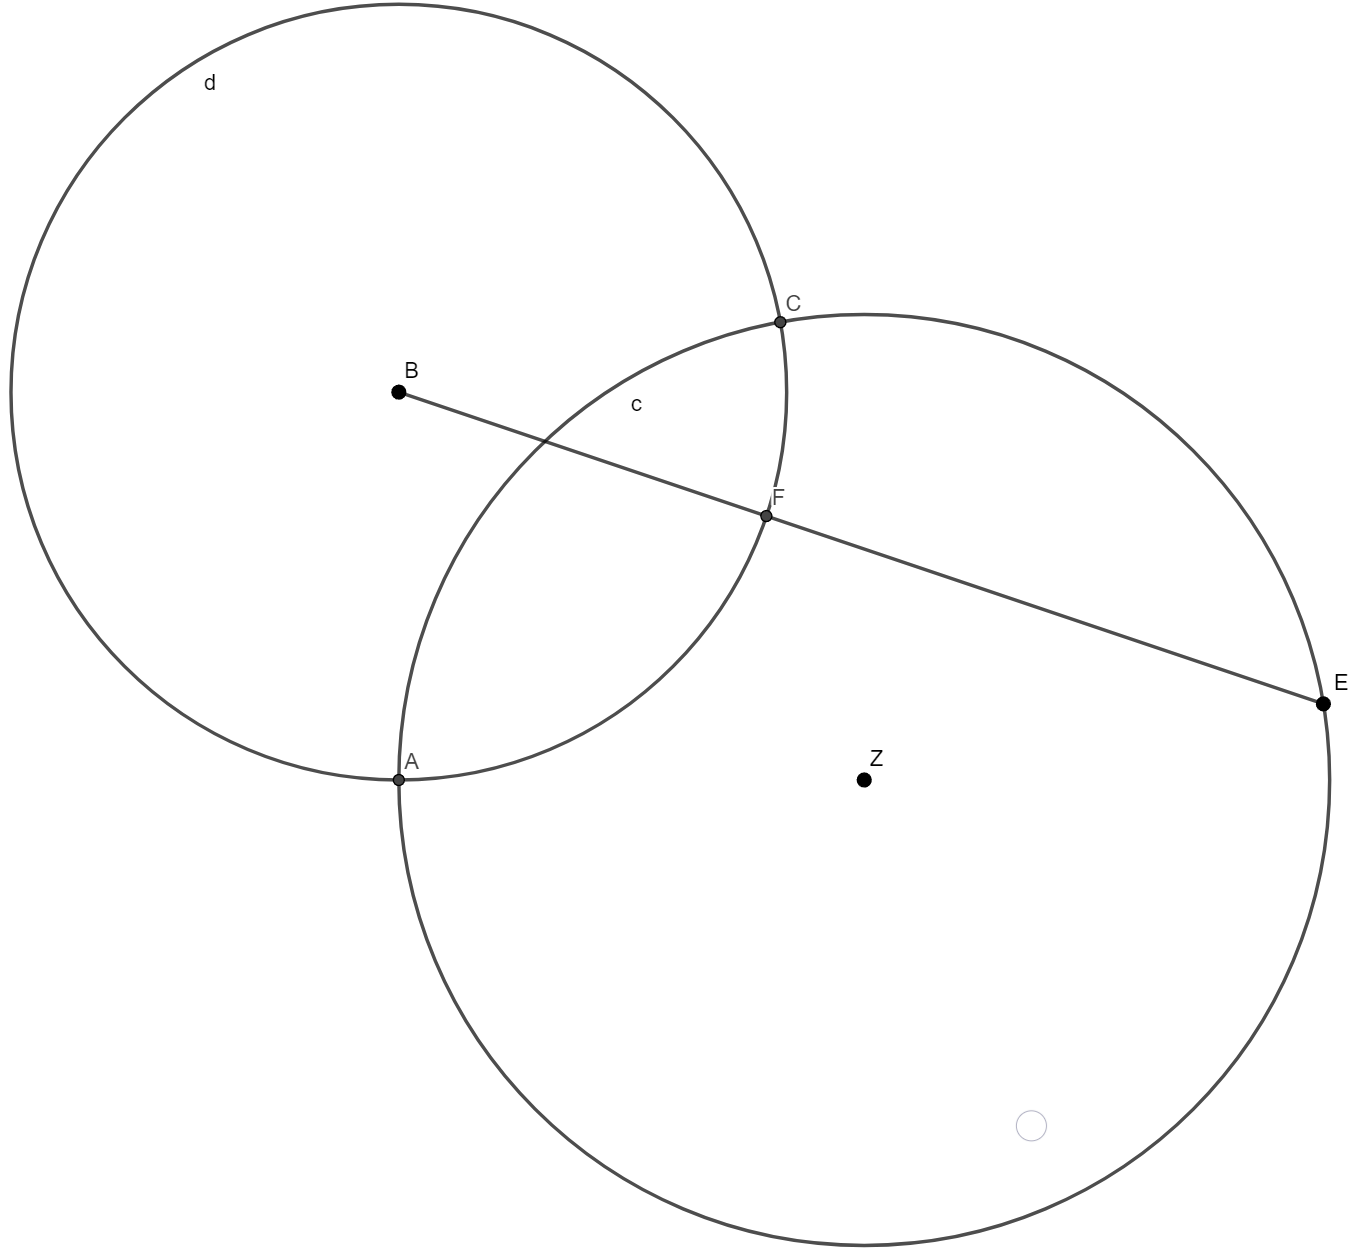
\includegraphics[scale=0.171,valign=t]{images/visual_proof_2.png}
    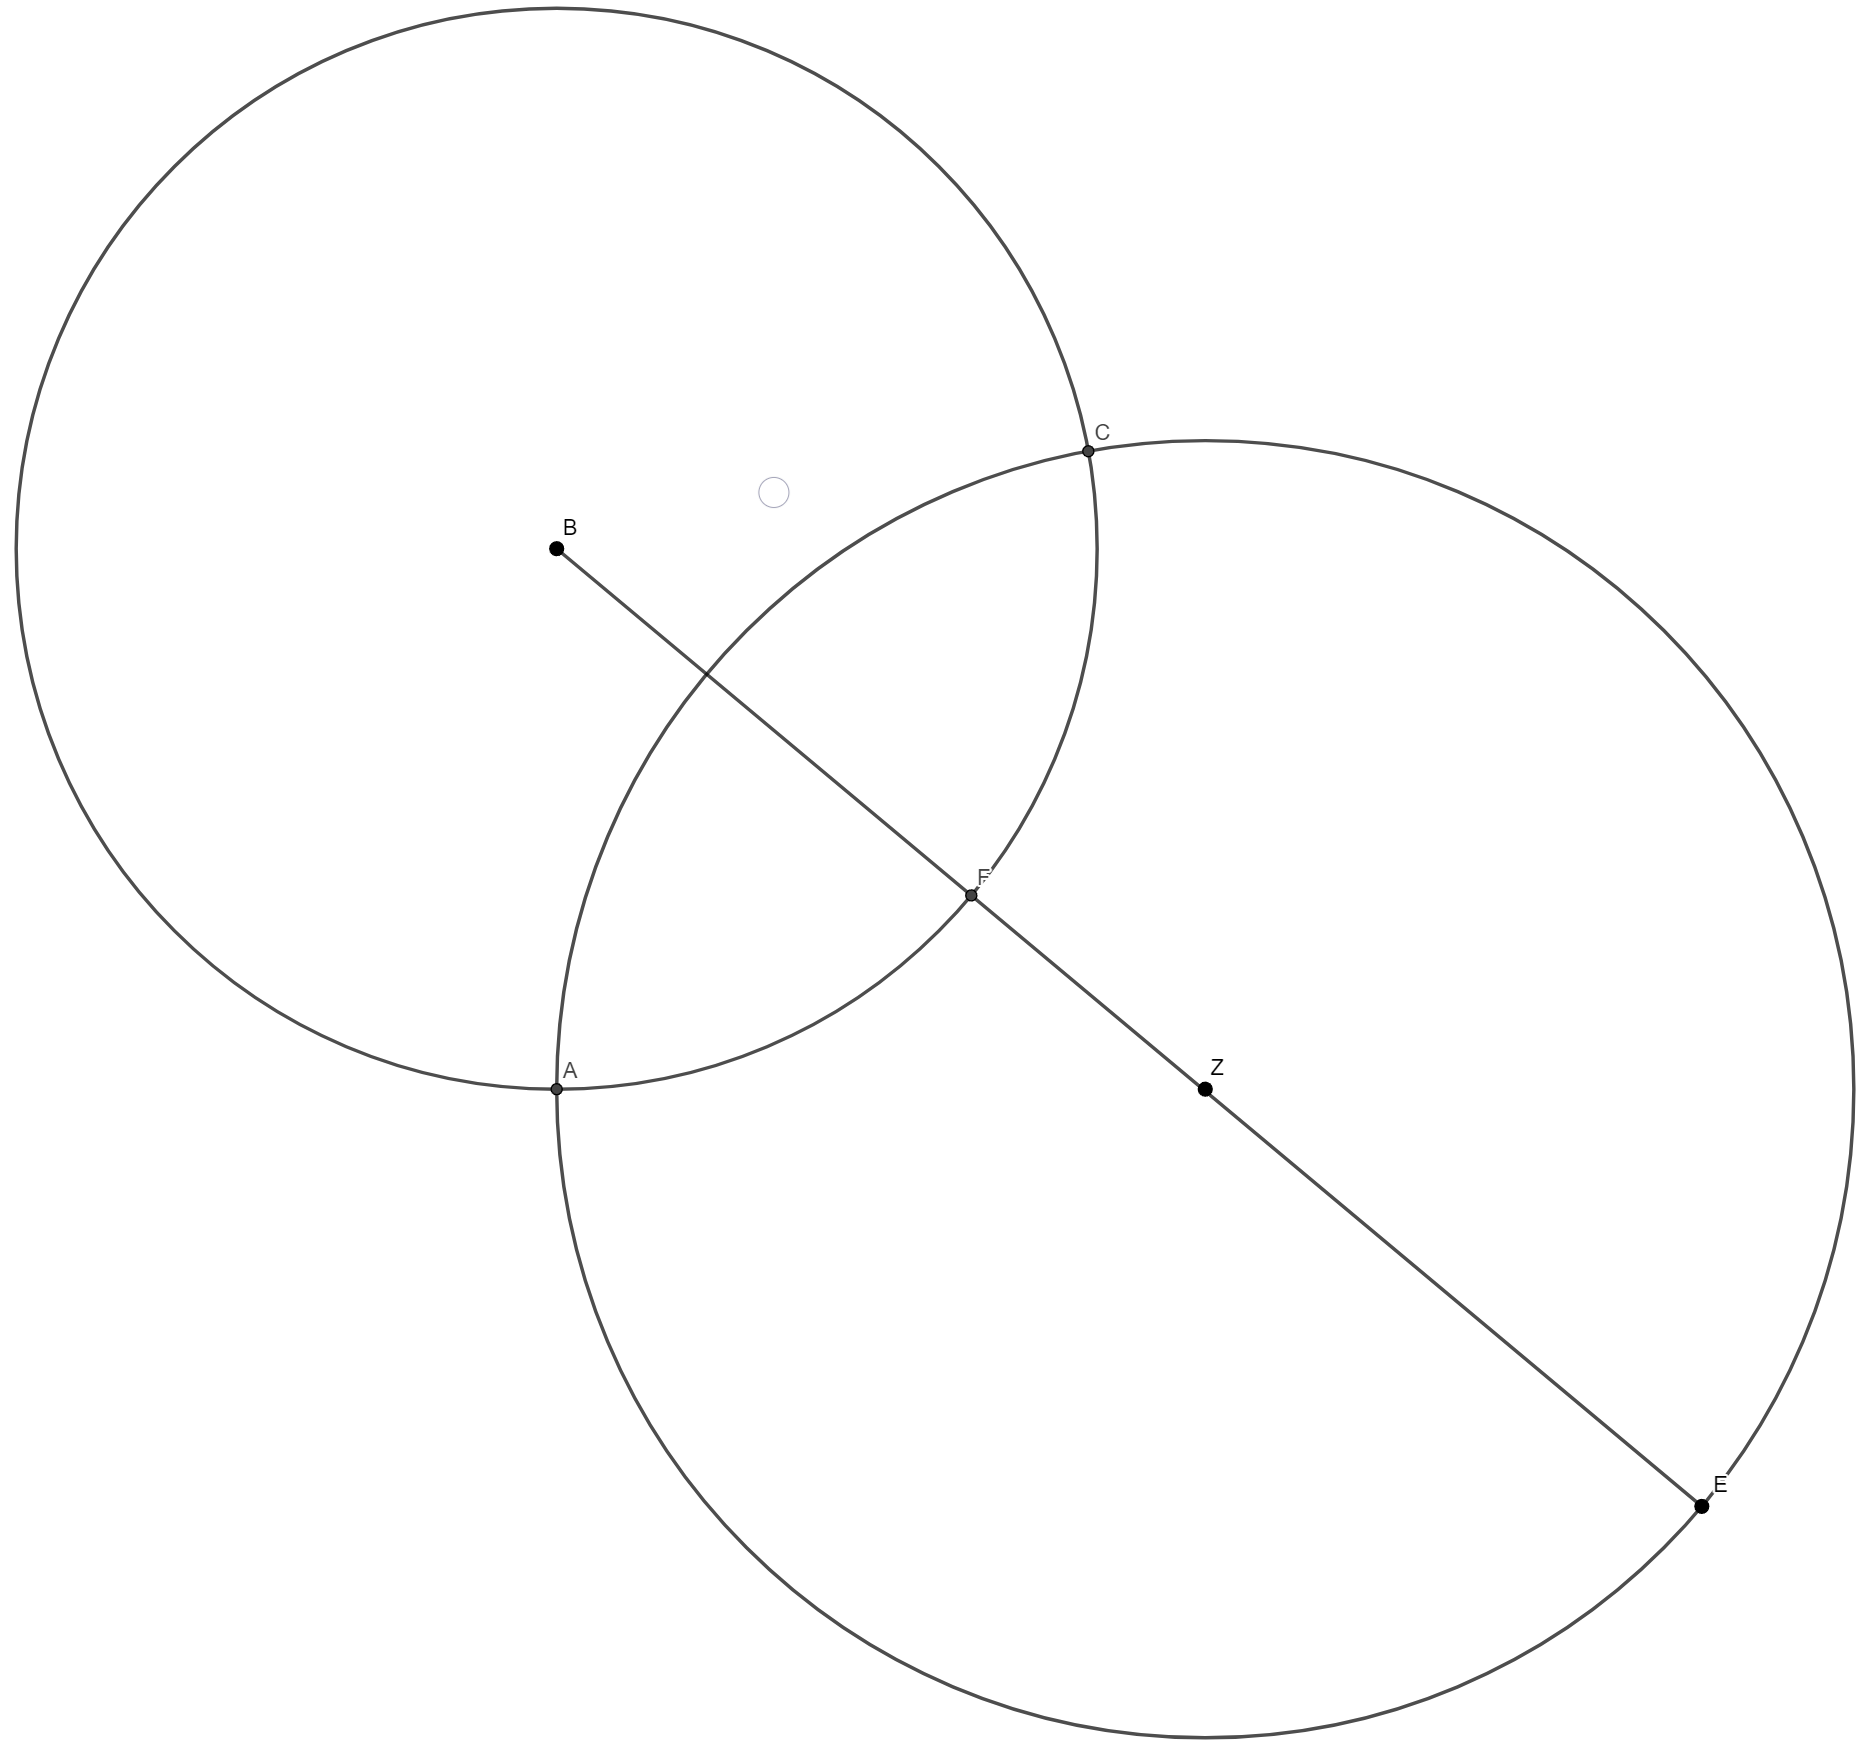
\includegraphics[scale=0.122,valign=t]{images/visual_proof.png}
    \caption{Dans le cas représenté, $r=1.2$. $[BE]$ et $[FE]$ à leur maximum sur la figure de droite, avec notamment $FE=2r-\frac{2}{3}$, comme l'explique le Théorème suivant avec $BF$, une constante égale à $1-\frac{1}{3}=\frac{2}{3}$.
      $[FE]\approx1.76$. Sur la figure de gauche, $[FE]$ ne passe pas par $Z$ est approximativement égal à $\approx1.52$.}
  \end{figure}

  On comprend donc que $[FE]$ est à son maximum lorsque qu'il passe par $Z$. On comprend aussi que $[FE]$ peut aussi représenter le diamètre d'un cercle placé à l'intérieur de $C_r$. On en déduit que pour assurer la formation d'un deuxième trajet circulaire dans $C_r$, sans
  que celui-ci ne dépasse $C_r$, il faut que l'appui soit au point $K$ inscrit sur la circonférence du cercle trigonométrique et passant par le segment formé à partir du centre du cercle trigonométrique et du centre du cercle $C_r$.
\end{proof}


\begin{theorem}
  $\forall r>\frac{4}{3}$, rayon du cercle $C_r$, il est possible d'inscrire un cercle de rayon 1 à partir d'un trajet demi-circulaire, avec $n_{bouton}=1$.
\end{theorem}

\begin{proof}
  Nous nous baserons dans le cas où $r$ est à son minimal lorsque $n_{bouton}=1$. En d'autres termes, une partie du bord du cercle de rayon 1 avec un trajet stable qui touche du bord du cercle $C_r$ au rayon $r>0$. Soit une représentation
  semblable à celle ci-contre:

  \begin{figure}[H]
    \centering
    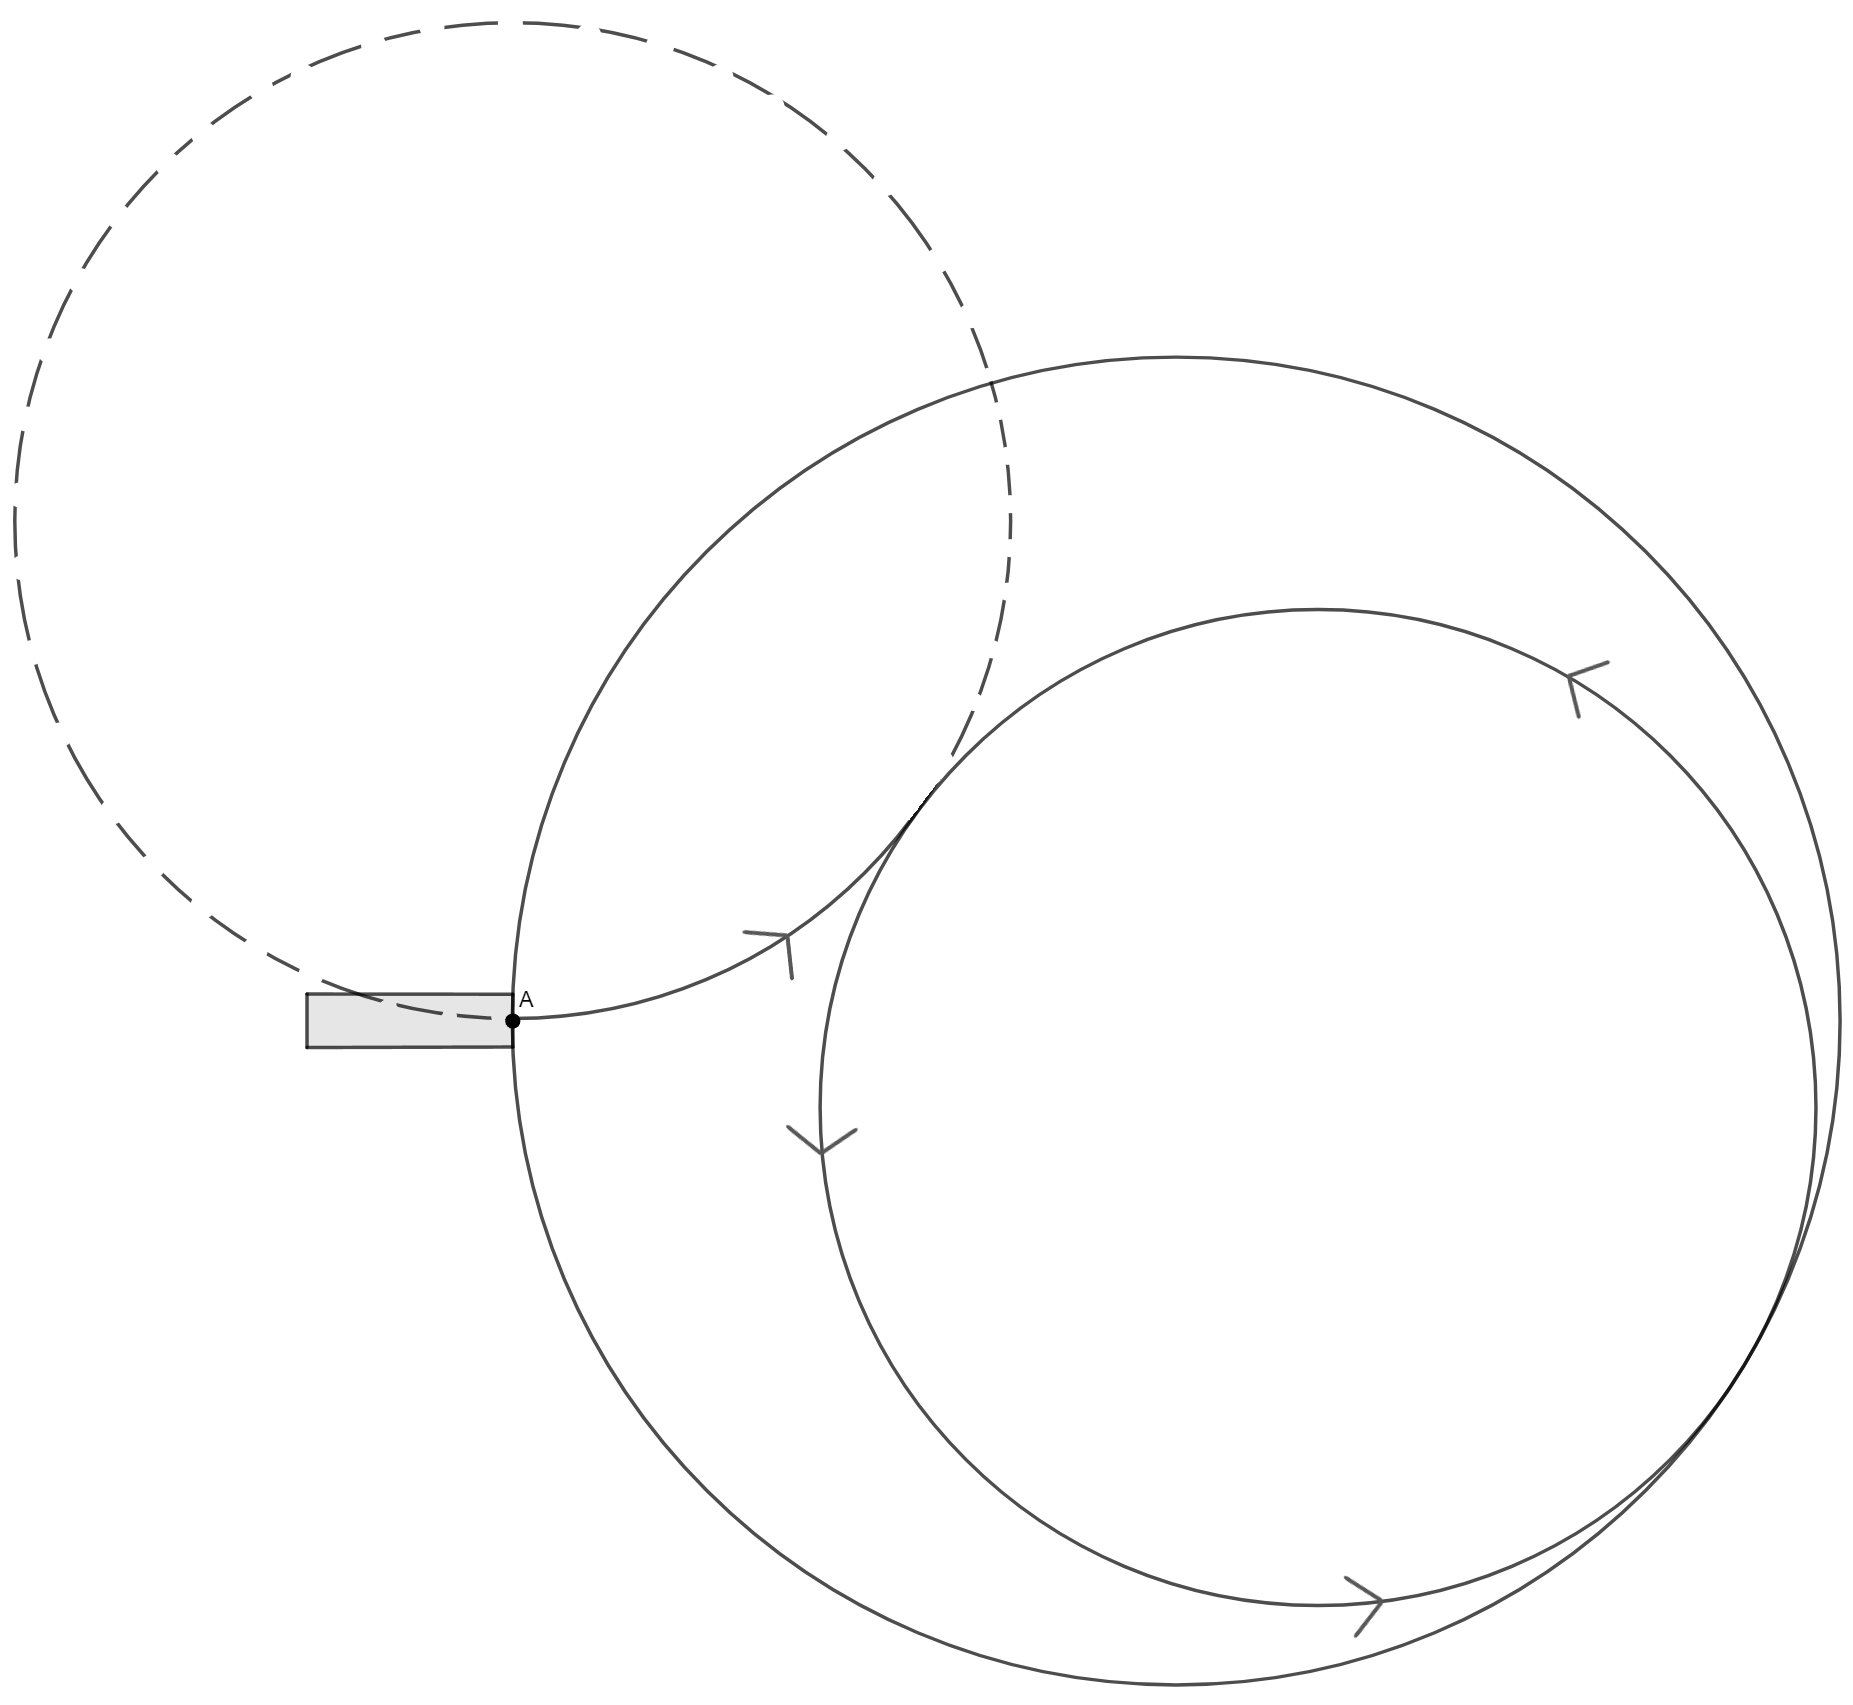
\includegraphics[scale=0.15]{images/perfect_inside.png}
    \caption{Trajet circulaire stable avec le cercle trigonométrique infiniment prôche du bord de $C_r$.}
  \end{figure}

  Soit $F$ point situé au centre du cercle formé par le premier trajet circulaire (lorsque $n_{bouton}=0$, au tir du canon), soit le point $G$ situé le centre
  du cercle formé par le deuxième trajet (lorsque $n_{bouton}=1$) et soit le point $Z$, le point situé au centre de $C_r$.

  Le point $F$ étant sur la tangente au point $A$ de $C_r$ et la tangente du premier trajet circulaire au point $A$ passant par le centre de $C_r$ (soit $Z$), on en déduit que
  le triangle $FAZ$ est rectangle en $A$. Soit $H$ sur la circonférence de $C_r$ tel que $F,Z,G,H$ soient alignés (selon le \textbf{Théorème 5.2}) (et que $r$, le rayon de $C_r$ est égal à $GH$). On définit aussi $y\in\mathbb{R^+_*}$ la longueur de la droite $FZ$ n'étant pas dans $C_r$. Voici une représentation des objets géométriques ci-contre:

  \begin{figure}[H]
    \centering
    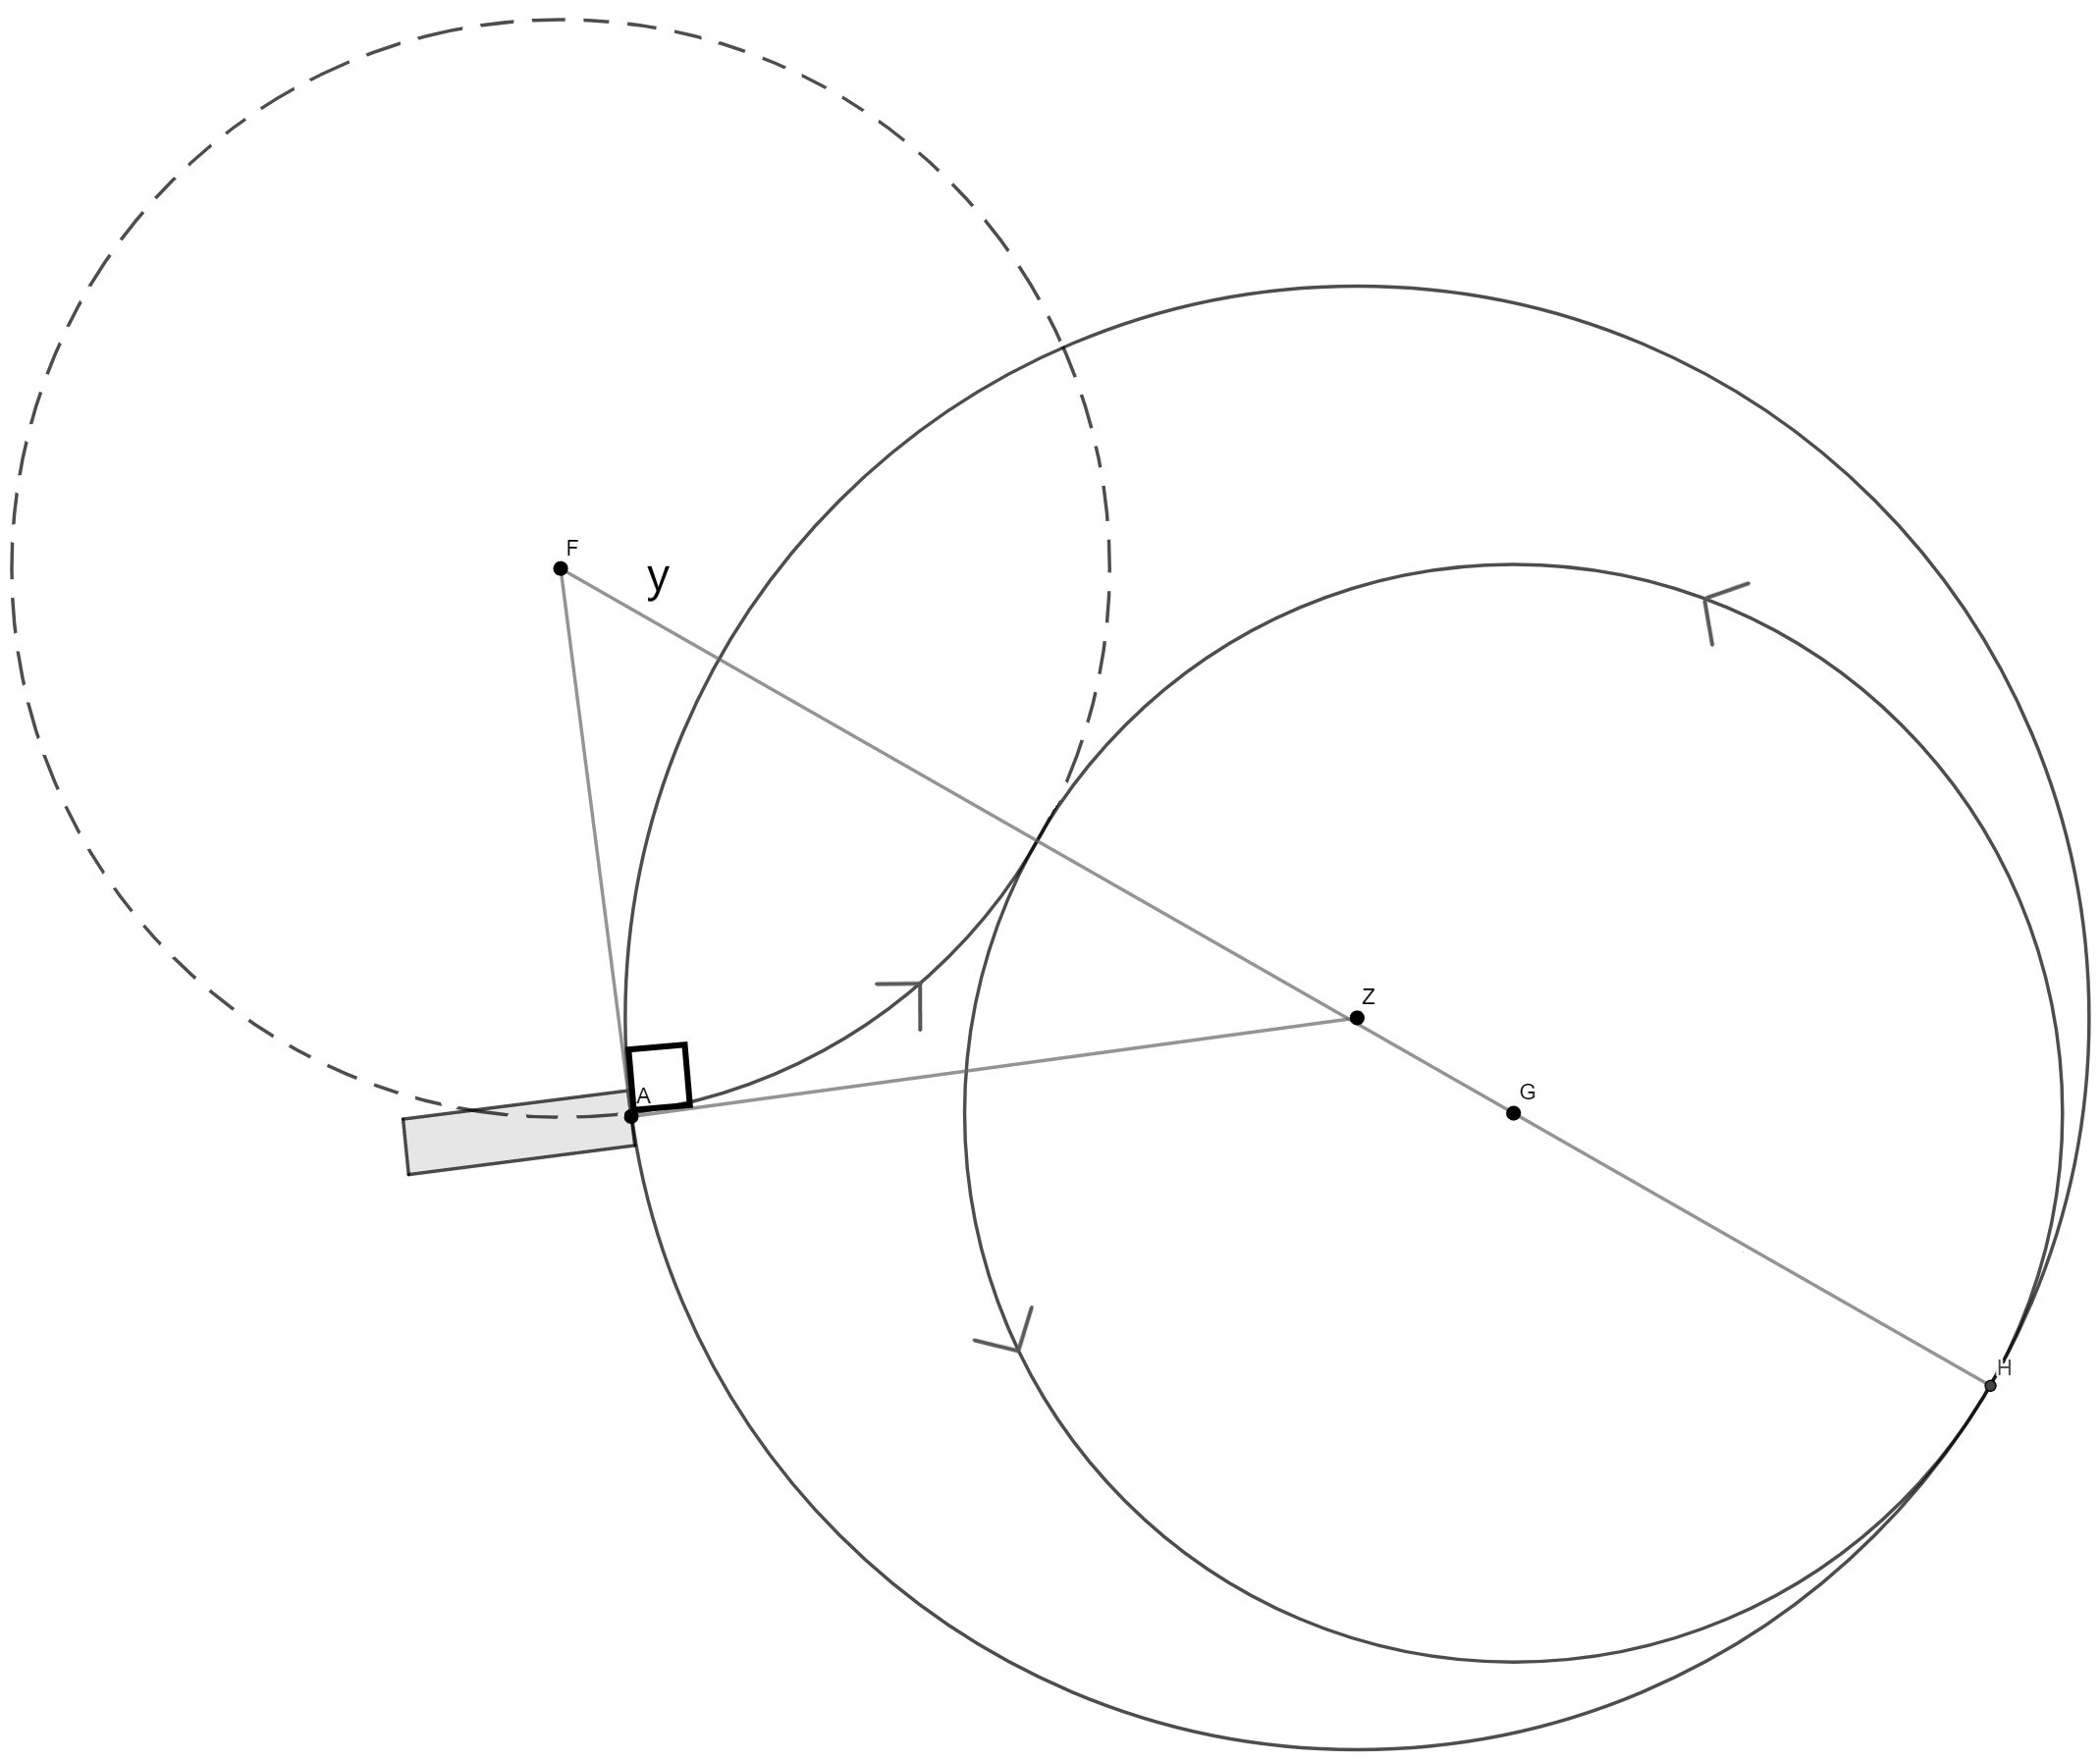
\includegraphics[scale=0.15]{images/q2_representation.png}
    \caption{$FAZ$ est un triangle rectangle.}
  \end{figure}

  Sachant que $r$ est le rayon de $C_r$, ques le cercles des deux trajets ont un rayon $r^\prime=1$ et que $y$ représente la longueur extérieure à la droite $FZ$, on comprend que:

  \[2ZH=FG+GH-y \Leftrightarrow 2r=3-y \Leftrightarrow r=\frac{3-y}{2}\]

  Ainsi que, $FAZ$ étant un triangle rectangle, d'après le Théorème de Pythagore:

  \[FZ^2=AZ^2+FA^2 \Leftrightarrow (r+y)^2=1+r^2 \Leftrightarrow r=\frac{1-y^2}{2y}\]

  En regroupant les égalités, nous trouvons que:

  \[\frac{3-y}{2}=\frac{1-y^2}{2y}\Leftrightarrow y=\frac{1}{3}\]

  Soit donc:

  \[ r=\frac{3-y}{2}\Leftrightarrow r=\frac{3-\frac{1}{3}}{2} \Leftrightarrow r=\frac{4}{3}\]

  On comprend donc que le rayon $r$ de $C_r$ doit être égal à $\frac{4}{3}$ afin que le trajet stable de l'électron touche le bord de $C_r$. On en déduit que $r$ doit nécessairement être supérieur à $\frac{4}{3}$ afin que l'électron ne touche pas son bord.
  Soit:

  \[r>\frac{4}{3}\]

  Avec $n_{bouton}=1$.
\end{proof}

\begin{conjecture}
  Il est possible d'avoir un trajet stable lorsque $\forall r\leq\frac{4}{3}$ avec $n_{bouton}=n$, $n\in\mathbb{N}$ et $n$, un grand nombre.
\end{conjecture}

L'égalité avec $n_{bouton}=1$ et $r>\frac{4}{3}$ ne laisse pas dors-et-déjà induire l'idée qu'il s'agit du rayon minimal même quand $n_{bouton}\to +\infty$. Si l'on souhaite faire une visualisation simple des possibilité, nous trouvons une représentation semblable à celle ci-dessous:

\begin{figure}[H]
  \centering
  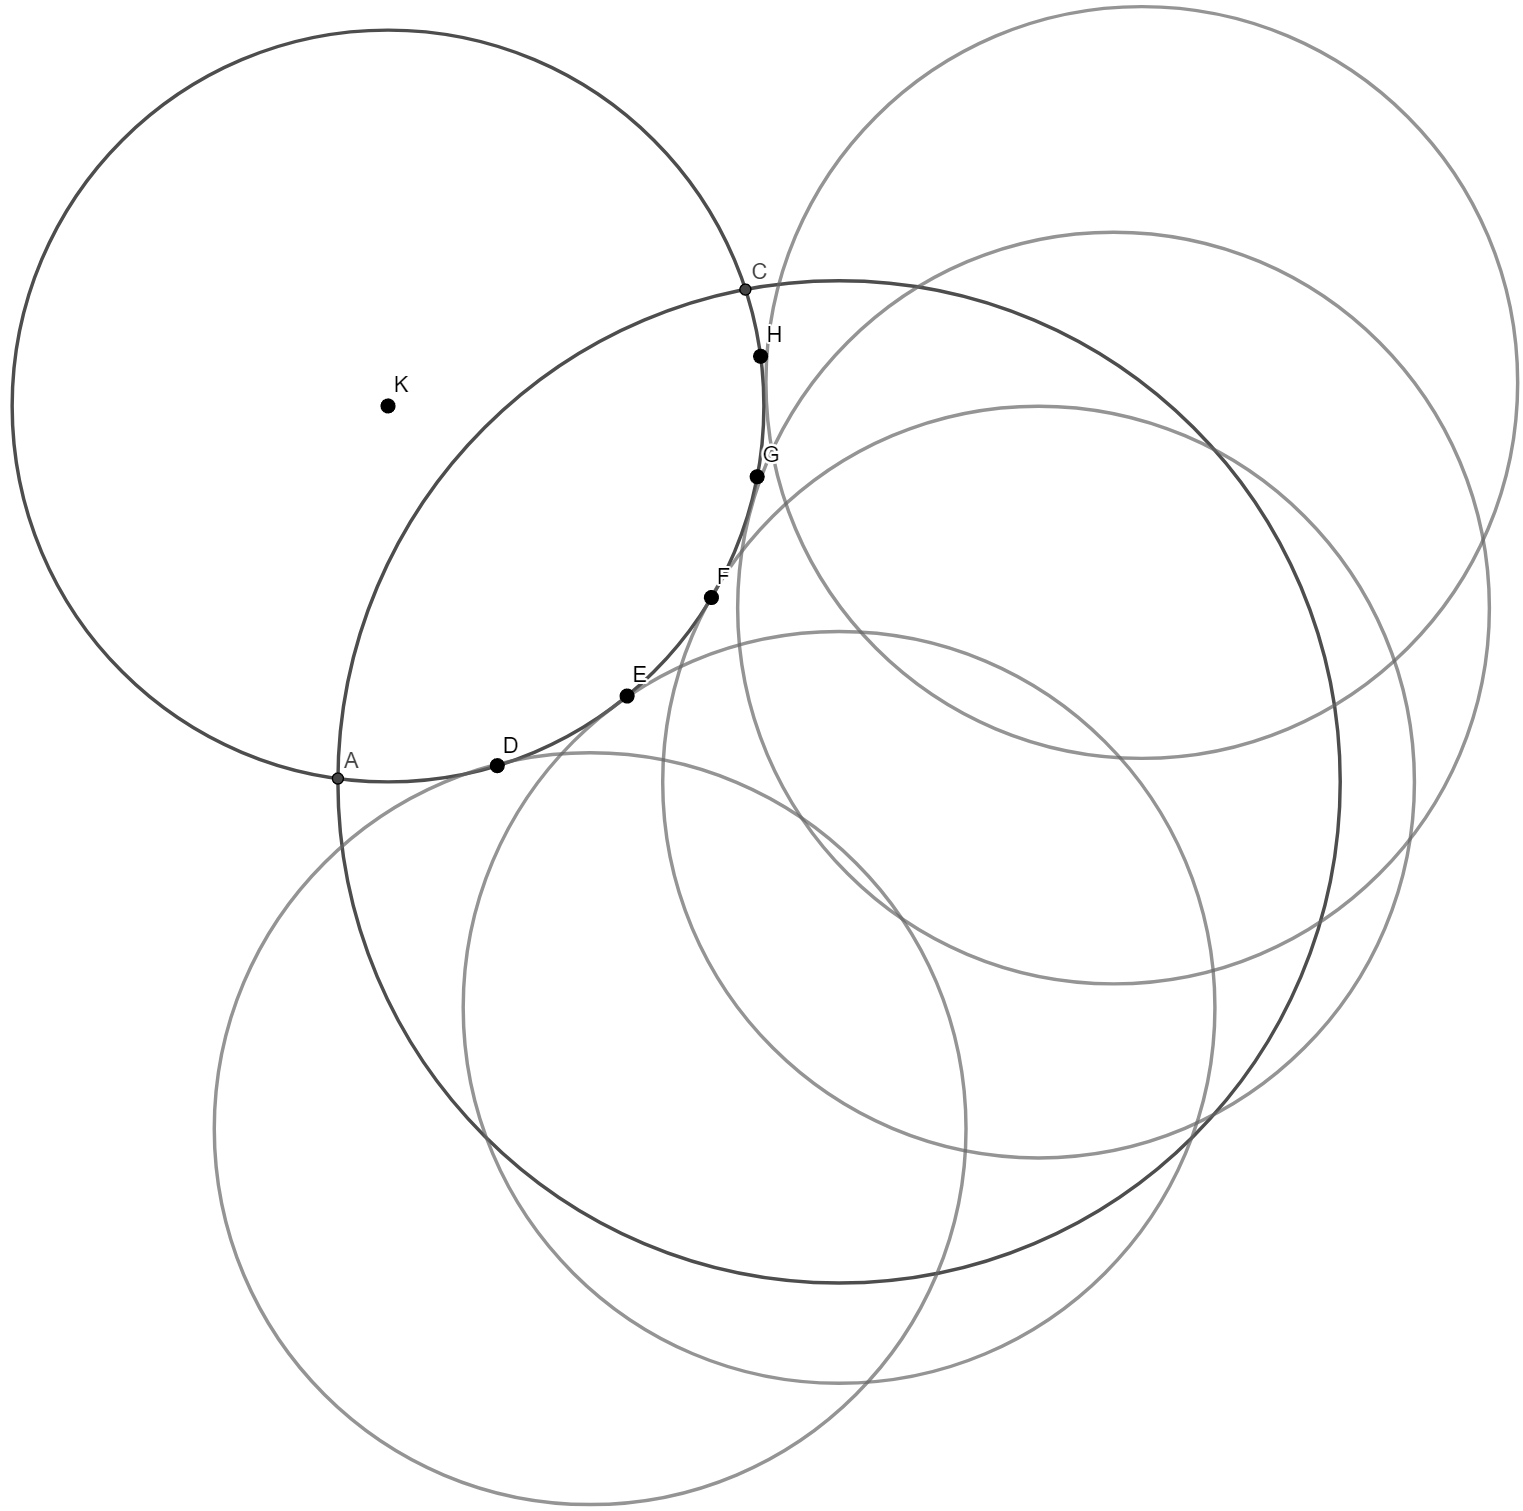
\includegraphics[scale=0.2]{images/conjecture.png}
  \caption{Représentation simple des possibilités lorsque $n_{bouton}=1$. $D,E,F,G,H$ sont des points auxquels Nicolas a appuyé sur son bouton. Dans le cas ci-dessous, $r=\frac{4}{3}$.}
\end{figure}

Avec une simple visualisation des autres cercles que l'on aimerait former à partir de ces trajets, il semble tout de même possible de placer un cercle de rayon $r\leq\frac{4}{3}$. En effet on peut même supposer qu'il soit possible d'avoir un trajet stable lorsque $r\to1$ (et non pas $r=1$ car dans un tel cas, le trajet touche les bords de $C_r$), avec dans un tel cas,
le centre du cercle $C_r$ confondu avec le centre du dernier trajet circulaire stable.

Ce principe s'affirme d'autant plus notamment avec le \textbf{Théorème 9.1}.

\section{Réponse à la Question 2}

Comme l'explique le \textbf{Théorème 5.3}, pour toute valeur $r>\frac{4}{3}$, Nicolas peut assurer un trajet stable (l'électron ne touche jamais le cercle) en appuyant un nombre fini de fois.

À partir du même Théorème, on comprend que pour Nicolas doit appuyer au moins une fois sur le bouton (et non pas 0 fois comme l'assure le \textbf{Théorème 5.1}), soit donc $n_{bouton}=1$.

Cependant, comme l'explique la \textbf{Conjecture 5.4}, il n'est pas certains que Nicolas ne puisse jamais trouver un autre trajet stable avec $r\leq\frac{4}{3}$ et $n_{bouton}>1$.

\section{Théorèmes pour la Question 3}

\textit{Remarque.} Selon la \textbf{Définition 2.4}, $N$ (selon la question) et $n_{bouton}$ représentent la même information dans le cadre de cette question. Nous appelons aussi $r_D$ ce que l'énoncé appelle $R$.
\begin{theorem}
  Avec $n=0 $ ou $n=1$ points placés strictement à l'intérieur d'un disque $D$ de rayon $r_D\leq1,r\in\mathbb{R^+_*}$, le plus petit $N\in\mathbb{N}$ tel que quelle que soit la
  position des $n$ points, on peut s’assurer que l’électron passe par ces $n$ points en appuyant au plus $N$ fois est $N=0$.
\end{theorem}

\begin{proof}
  Lorsque $n=0$, il n'y a pas de points dans le disque $D$. On considère par défaut qu'il n'aura pas besoin de tir et que $N=0$.

  Lorsque $n=1$, il existe qu'un unique point $n_0$ dans le disque. On considère l'emplacement du canon tel que le point $A$, départ du trajet de l'électron soit confondu ou infiniment prôche à ce point pour que le trajet traverse ce dernier.
\end{proof}

\begin{theorem}
  Avec $n\in\mathbb{N}\backslash\lbrace{1,2}\rbrace$ points placés strictement à l'intérieur d'un disque $D$ de rayon $r_D\leq1, r\in\mathbb{R^+_*}$, le plus petit $N\in\mathbb{N}$ tel que quelle que soit la
  position des $n$ points, on peut s’assurer que l’électron passe par ces $n$ points en appuyant au plus $N$ fois sur le bouton est $N=n-2$.
\end{theorem}

\begin{proof}
  On place le canon tel que le point $A$, départ du trajet de l'électron soit confondu ou infiniment prôche au premier point ($n_0$) et on s'arrange qu'il soit orienté vers le deuxième car, comme l'explique le \textbf{Théorème 3.4}, on peut atteindre n'importe quel point avec une distance $d\leq2$ de $A$, soit une aire (ou un autre disque de surface $S=4\pi$).

  \begin{figure}[H]
    \centering
    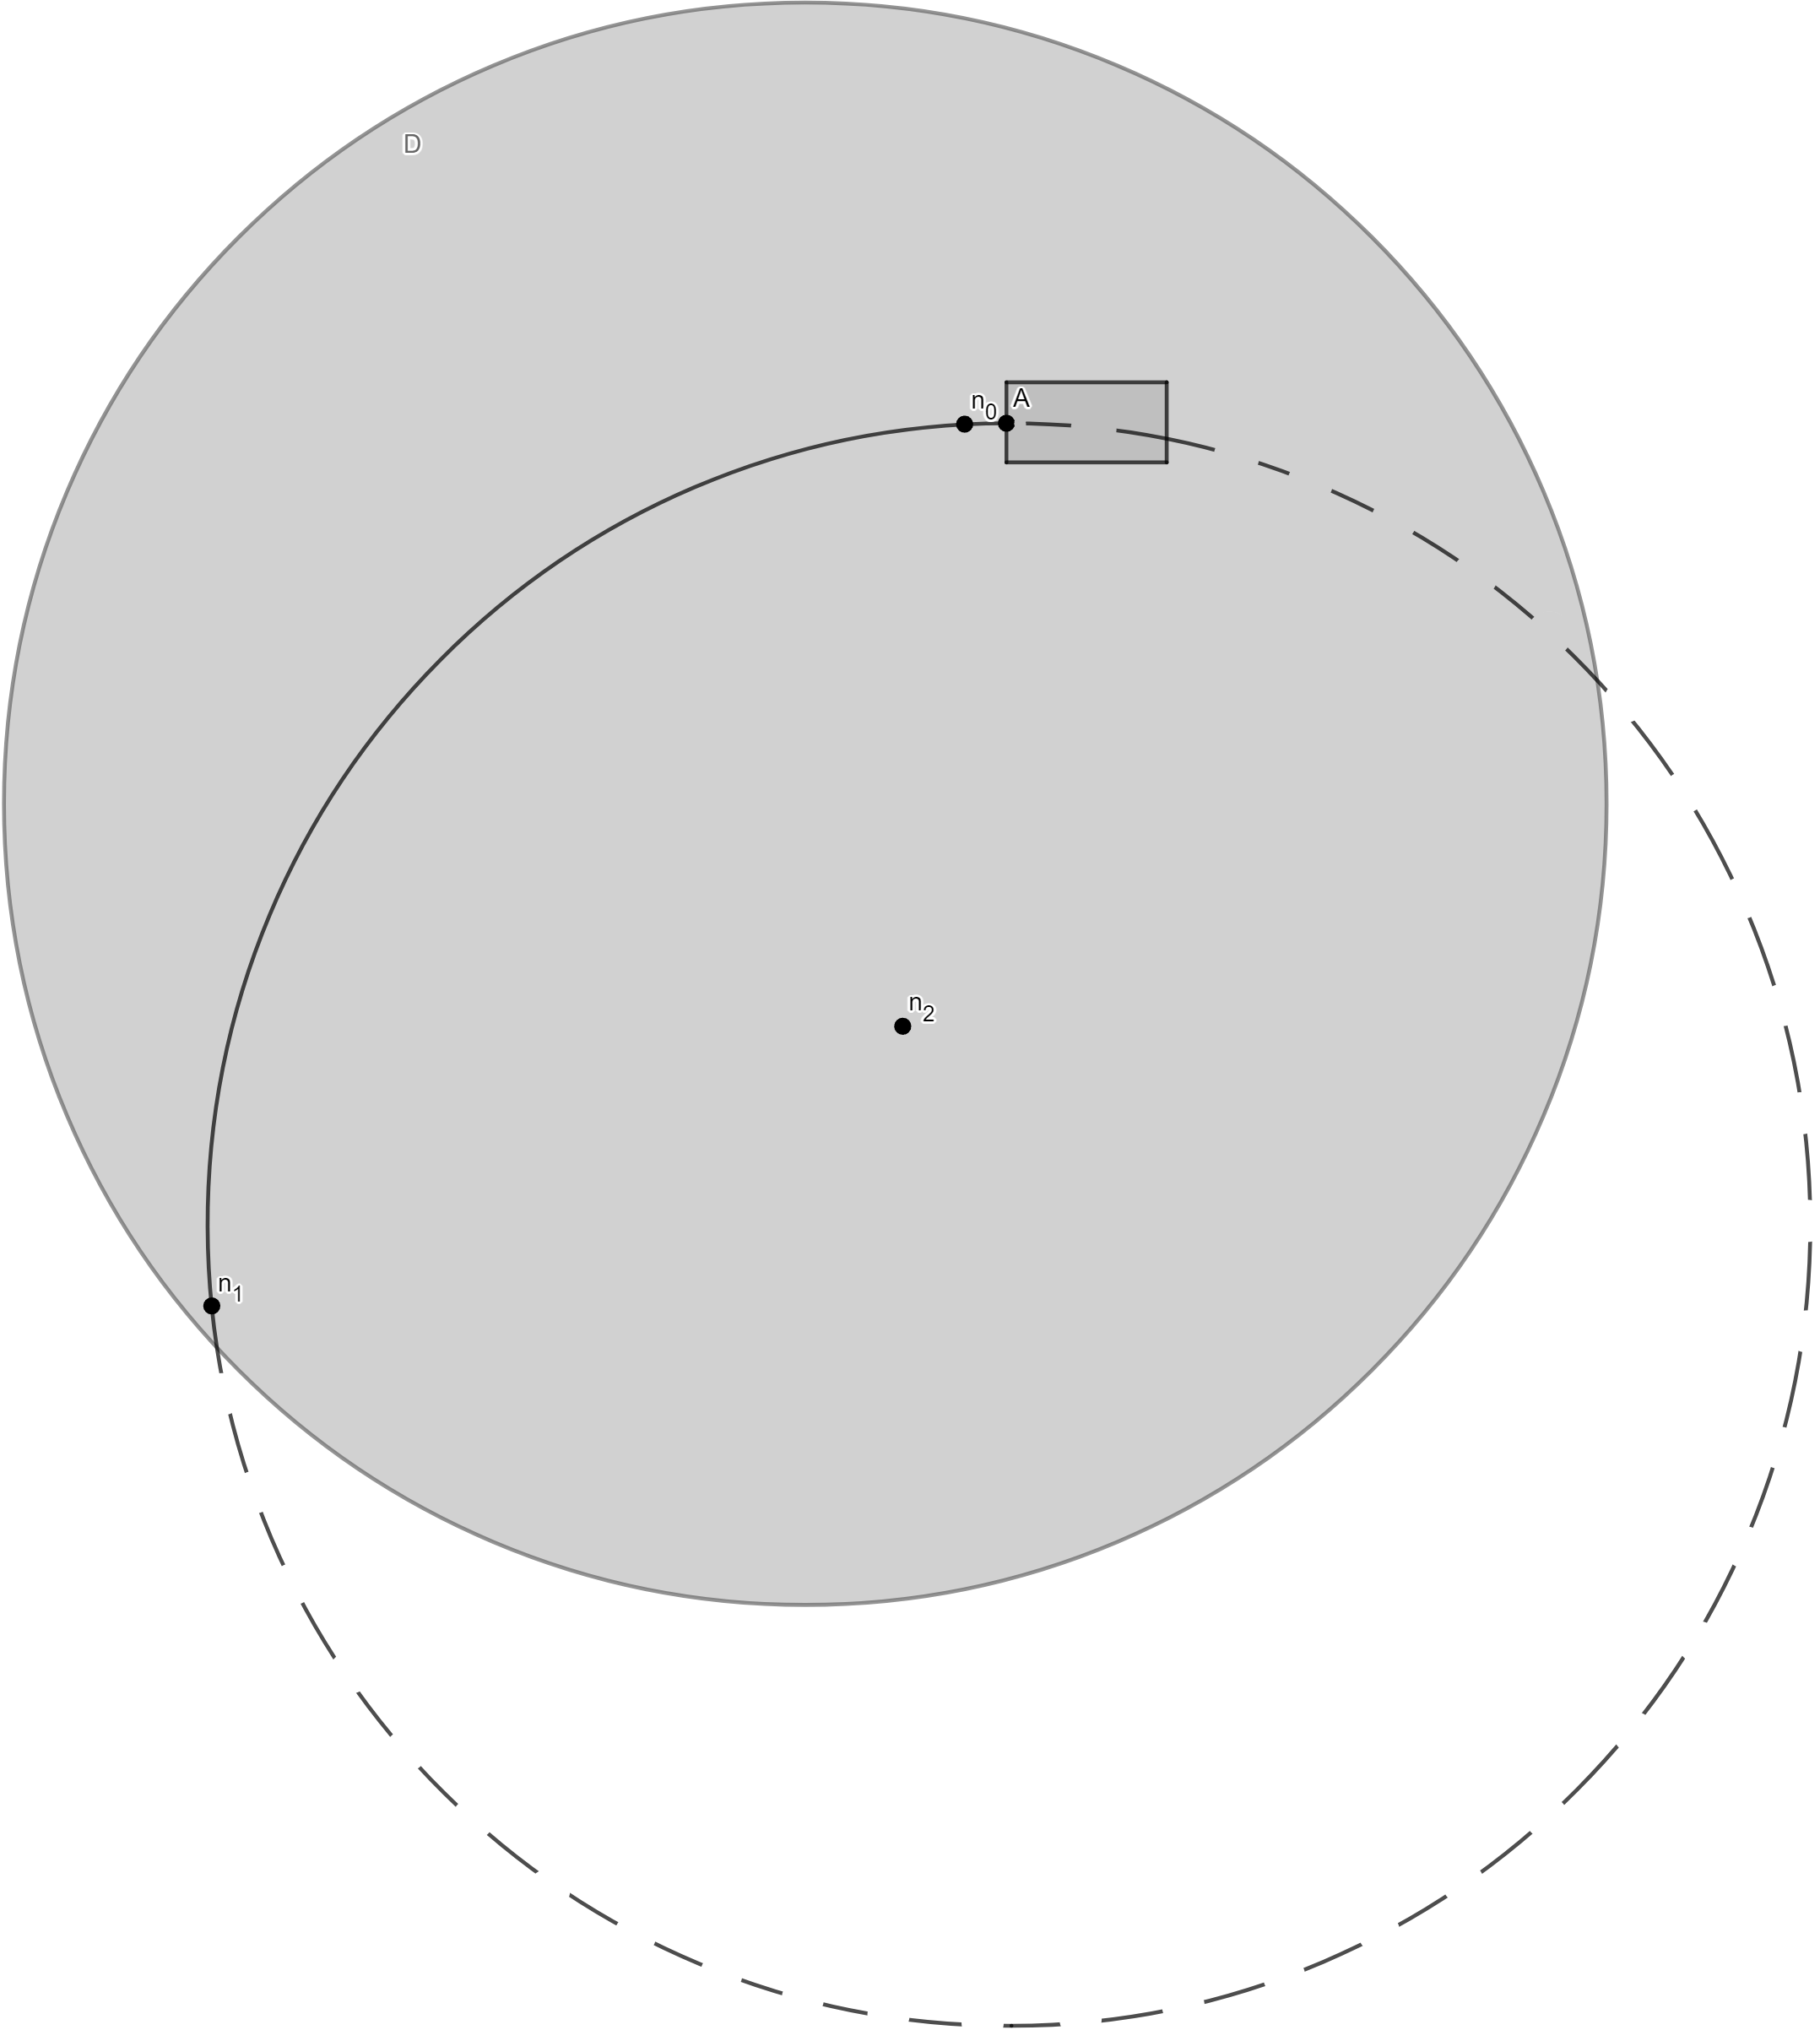
\includegraphics[scale=0.105]{images/q3.png}
    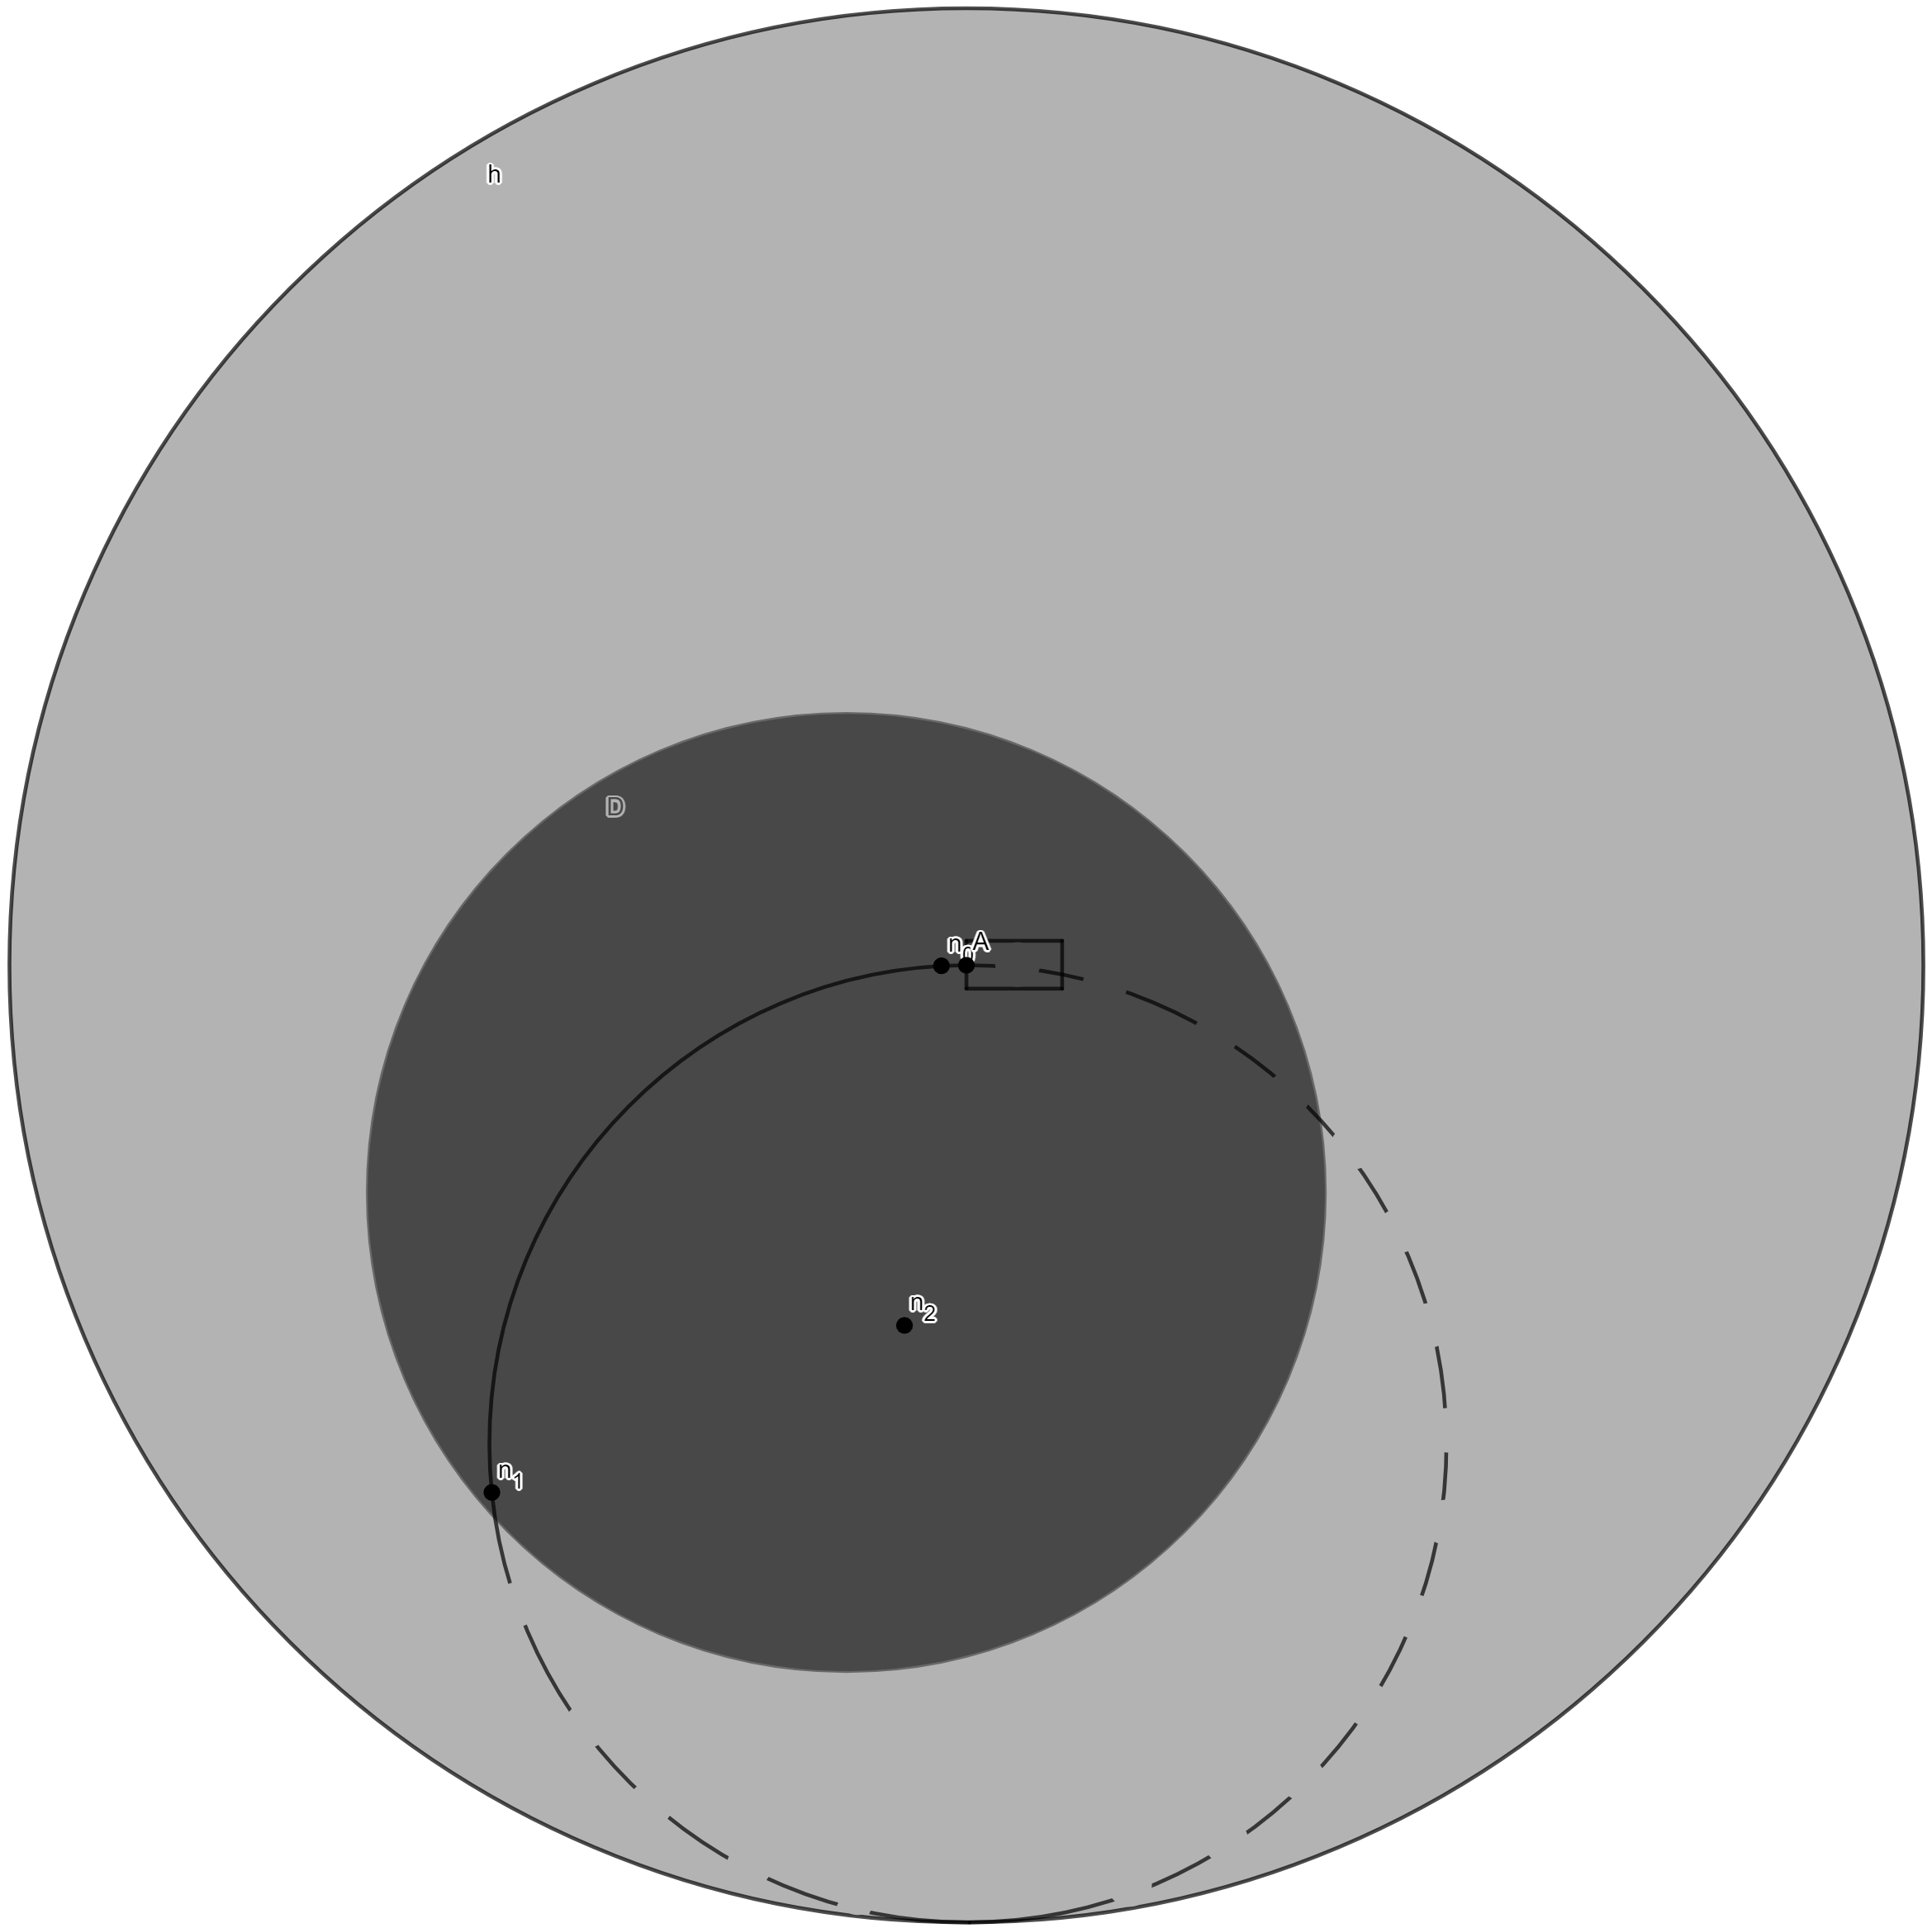
\includegraphics[scale=0.105]{images/q3_generalization.png}
    \caption{La figure de gauche montre qu'il est possible d'avoir un trajet associant deux points $n_0$ et $n_1$, tout en montrant un contre exemple dans le cas où l'électron pourrait passer par trois points (ne passe pas par $n_2$), avec $r_D=1$. (Notez aussi que dans un tel cas, nous n'avons pas confondu les points $n_0$ et $A$.)
    . \\La figure de droite est la même représentation à l'exception du rajout du disque $h$ de centre $A$ avec sa surface représentant tous les points que l'on peut atteindre d'un seul petit trajet à partir d'un point $A$ (selon le cas où $n_{bouton}=0$ du \textbf{Théorème 3.4}).}
  \end{figure}

  On remarque clairement que lorsque $N=0$, nous pouvons nous arranger pour atteindre au moins deux points $n_0,n_1$ inscrits strictement dans le disque $D$. Cependant, comme illustre la représentation de gauche de la Figure 21, nous ne pouvons pas 
  toujours atteindre un troisième point $n_2$, sauf s'il est, avec chance, sur le trajet de l'électron.

  On en déduit donc que l'on peut toujour s'assurer de passer par au moins deux points. D'où $N=n-2$ avec $n\in\mathbb{N}\backslash\lbrace{1,2}\rbrace$.
  Sinon, il sera obligé de re-appuyer sur le bouton pour passer sur un nouveau point. \\

  De plus, ce cas de figure est assez analogue au \textbf{Théorème 3.1}, avec la distance parcourue par le trajet selon la distance entre les deux points (Étant dans un disque de rayon $r_D$, on sait que les points peuvent au maximum avoir une distance $d=2r_D$, où dans le cas ici, $d\leq2$. On peut donc appliquer un tel Théorème).

  Si l'on souhaite exprimer la longueur du trajet entre les poits $n_0$ et $n_1$, on trouve que:

  \[d_{min A,n_1}=2\arcsin(\frac{d_{n_0,n_1}}{2})\]

  Selon le \textbf{Théorème 3.1}, avec $d_{min A,n_1}\in\mathbb{R^+}$, la longueur du trajet circulaire de $A$ à $n_0$, et $d_{n_0,n_1}\in\mathbb{R^+}$, la distance absolue entre les points $n_0$ et $n_1$. (Cela fonctionne car le point $A$ est confondu au point $n_0$, comme nous l'avons dit précédement.)
\end{proof}

\begin{theorem}
  Avec $n\in\mathbb{N}$ points placés strictement à l'intérieur d'un disque $D$ de rayon $r_D>1$, le plus petit $N\in\mathbb{N}$ tel que quelle que soit la
  position des $n$ points, on ne peut pas s’assurer que l’électron passe par ces $n$ points en appuyant au plus $N=n-2$ fois.
\end{theorem}

\begin{proof}
  Trouvons un contre-exemple. Dans le cas où $n=2$, on trouve que cela ne marche pas si l'on place ces points de tel sorte que la distance $d$ qui les sépare tend vers le diamètre du disque, soit $d\to2r_D$.

  Nous savons donc que $d>2$ et que le trajet, selon le \textbf{Théorème 3.4}, ne peut assurer que des points espacé de $2$ de distance avec $n_{bouton}=0$ (ou $N=0$). Voici une visualisation lorsque $r_D=1.1$:

  \begin{figure}[H]
    \centering
    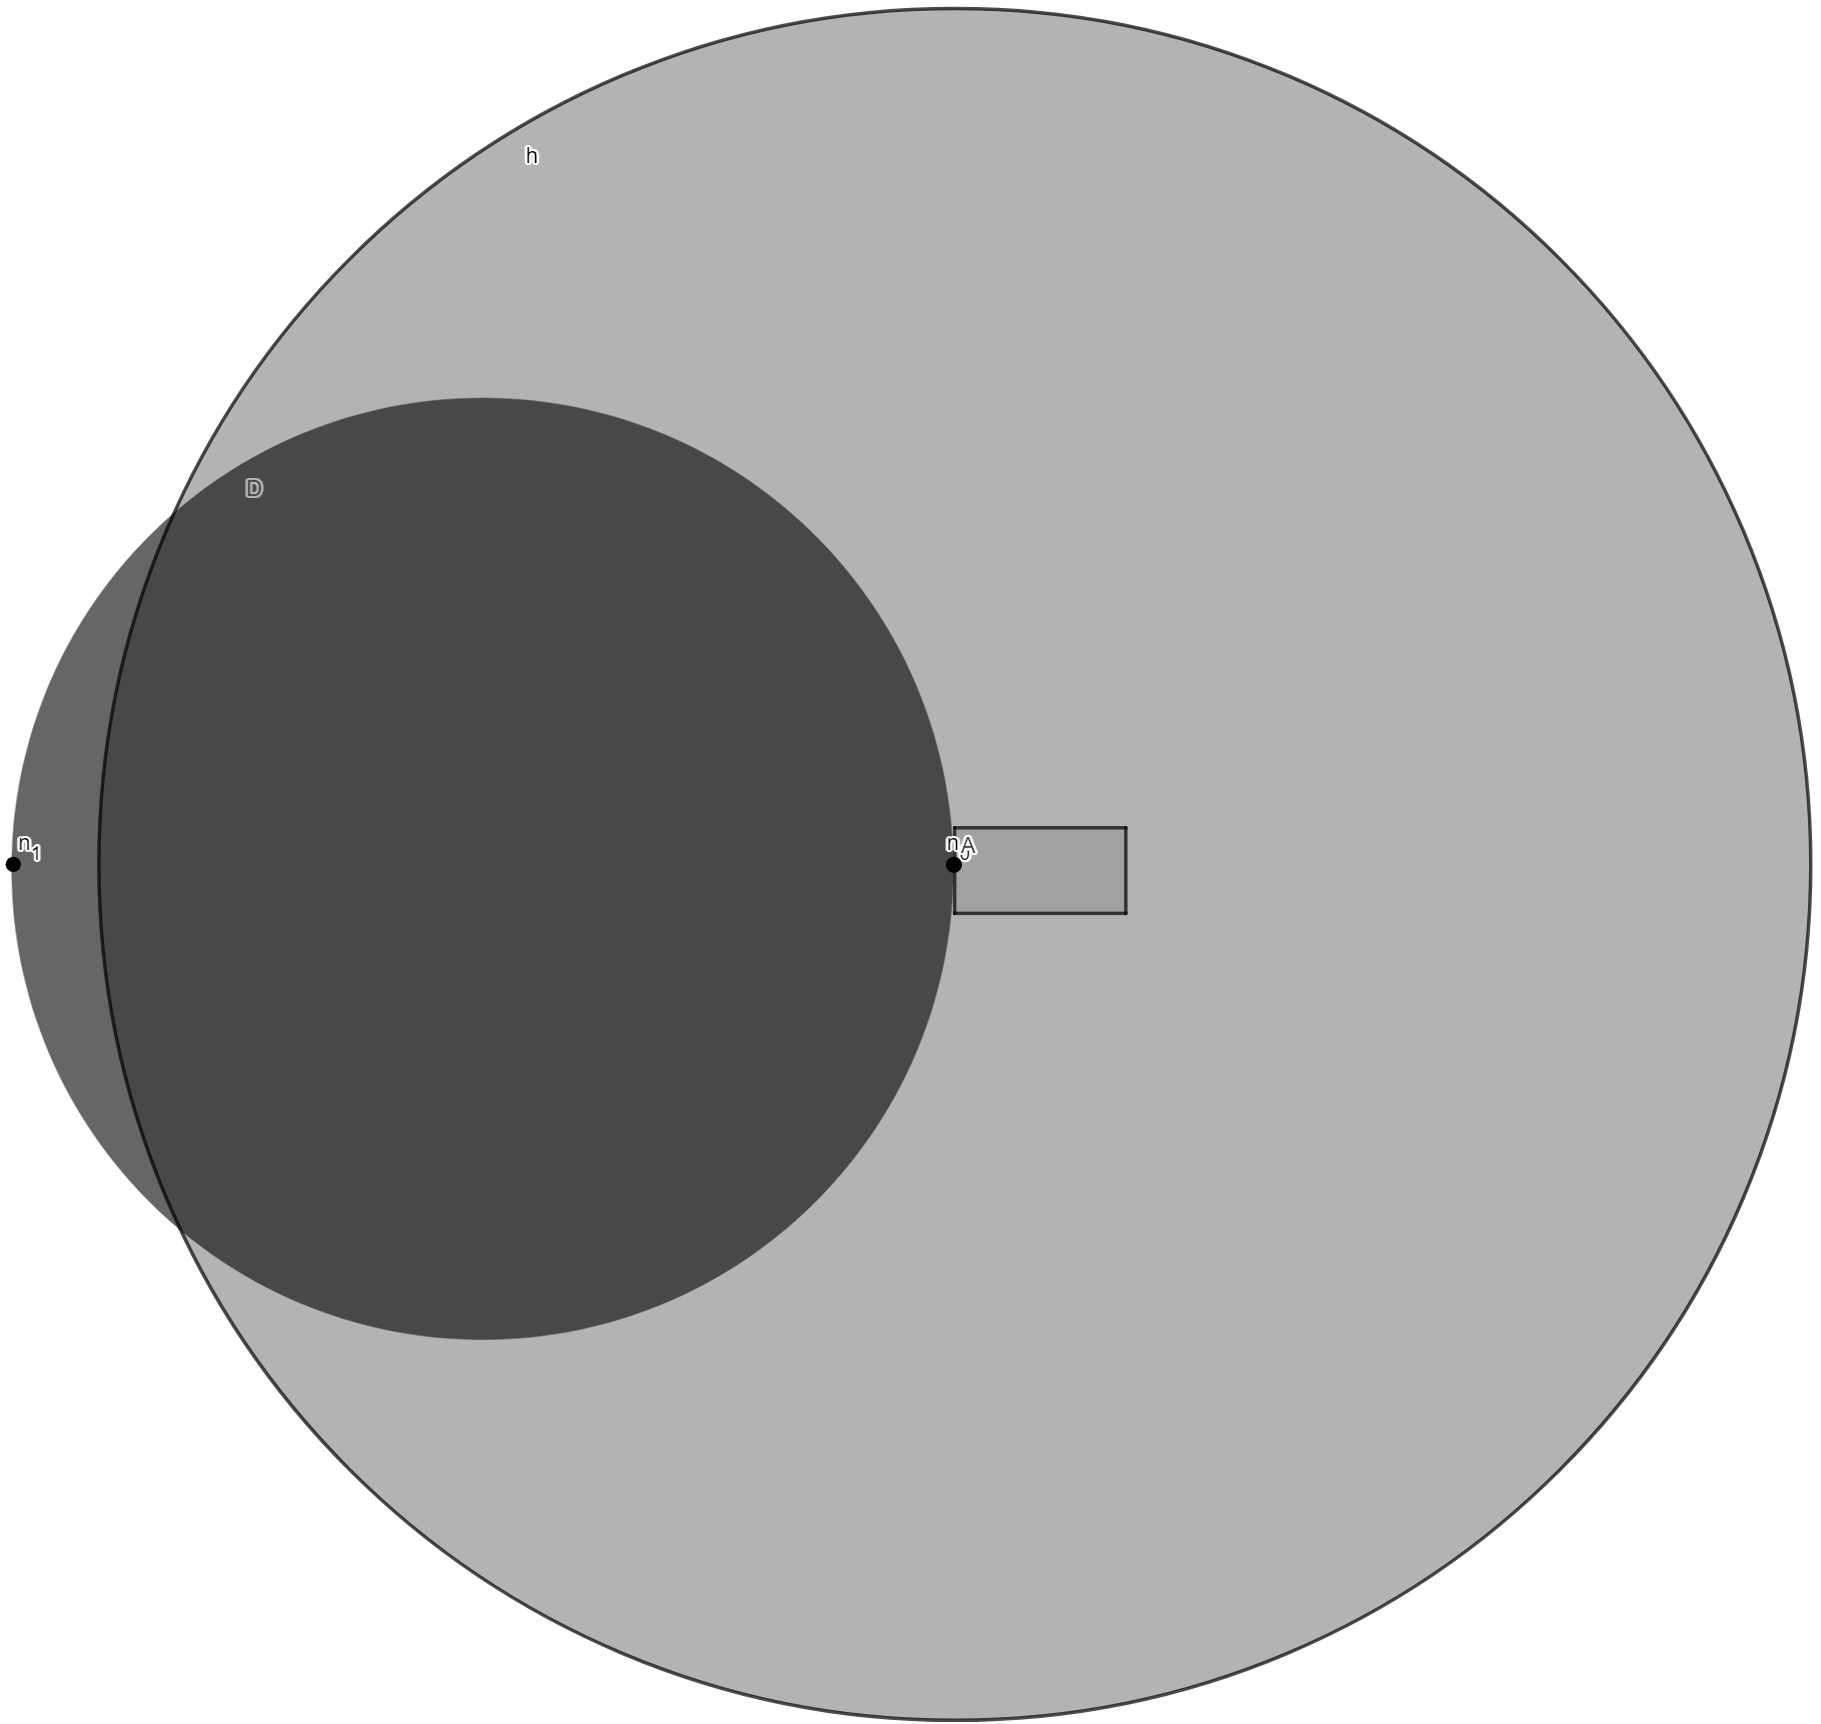
\includegraphics[scale=0.2]{images/q3_not_possible.png}
    \caption{Avec $n_0$ et $n_1$ espacés d'une distance qui tend vers le diamètre de $D$, il n'est pas possible de les joindre avec $N=0$. (On a aussi représenté la surface recouvrant l'ensemble des points que l'on peut toucher en partant de $A$, selon 
    le \textbf{Théorème 3.4}.)}
  \end{figure}

  On comprend donc que lorsque $n=2$, avec la formule trouvé au Théorème précédent, nous trouverions $N=n-2\Leftrightarrow N=0$, mais comme l'illustre la Figure 22, lorsque la distance $d$ entre ces deux points tend vers le diamètre, nous ne pouvons pas assurer
  le fait que le trajet passe par ces deux points avec $r_D>1$.
\end{proof}

\section{Réponse à la Question 3}

Lorsque $n=0$ ou $n=1$, le \textbf{Théorème 7.1} explique que l'on peut toujours passer par ces points avec points avec $N=0$.
Sinon, lorsque $n>1$, comme l'explique le \textbf{Théorème 7.2}, le plus petit entier $N$ tel que quelle que soit la position des $n$ points, on peut s’assurer que l’électron passe par ces $n$ points en appuyant
au plus $N$ fois sur le bouton est $N=n-2$ appuis. 

Afin de savoir ce qu'il se passe lorsque $r_D>0$, avec le \textbf{Théorème 7.2}, nous comprenons que lorsque $R\in]0;1]$, nous trouvons la même relation avec $N=n-2$. Cependant, lorsque $R>1$, le \textbf{Théorème 7.3} 
explique que la relation du \textbf{Théorème 7.2} ne marche plus.

\section{Théorèmes pour la Question 4}

\textit{Remarque.} Nous prenons pour $k\in\mathbb{N}\backslash\lbrace{1}\rbrace$, $k$ représentant le nombre de canons (et d'électrons).

\begin{theorem}
  Il est possible d'amener l'électron n'importe où dans le plan, même avec une orientation du canon fixée.
\end{theorem}

\begin{proof}

  Étant assez difficile d'effectuer une démonstration algébrique sur ce principe, nous nous munierons de représentations:

  \begin{figure}[H]
    \centering
    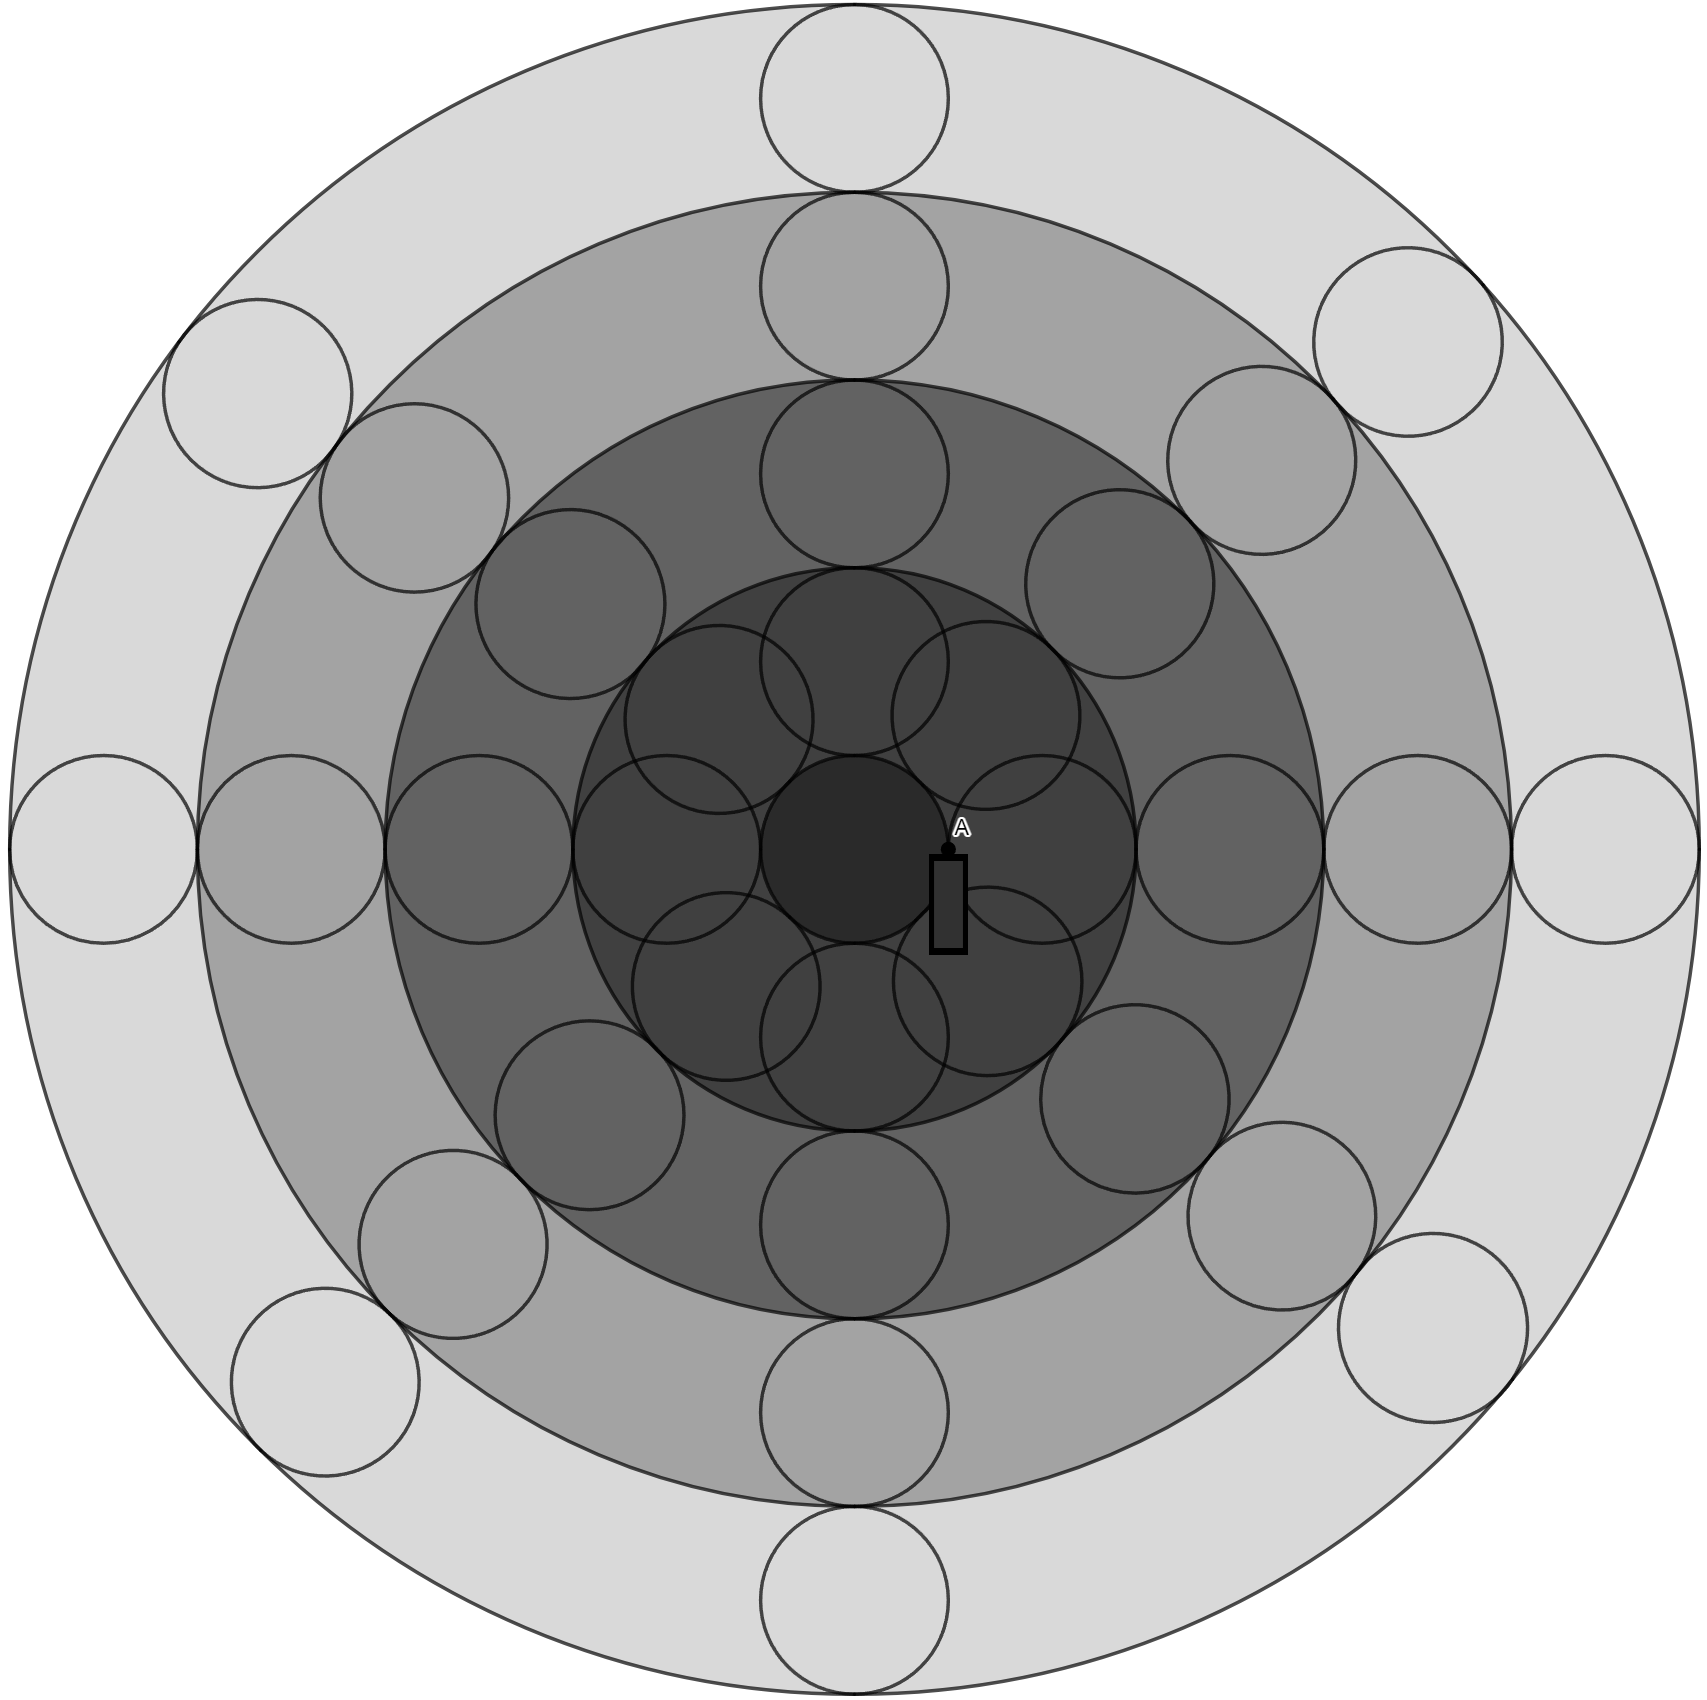
\includegraphics[scale=0.13]{images/it_can.png}
    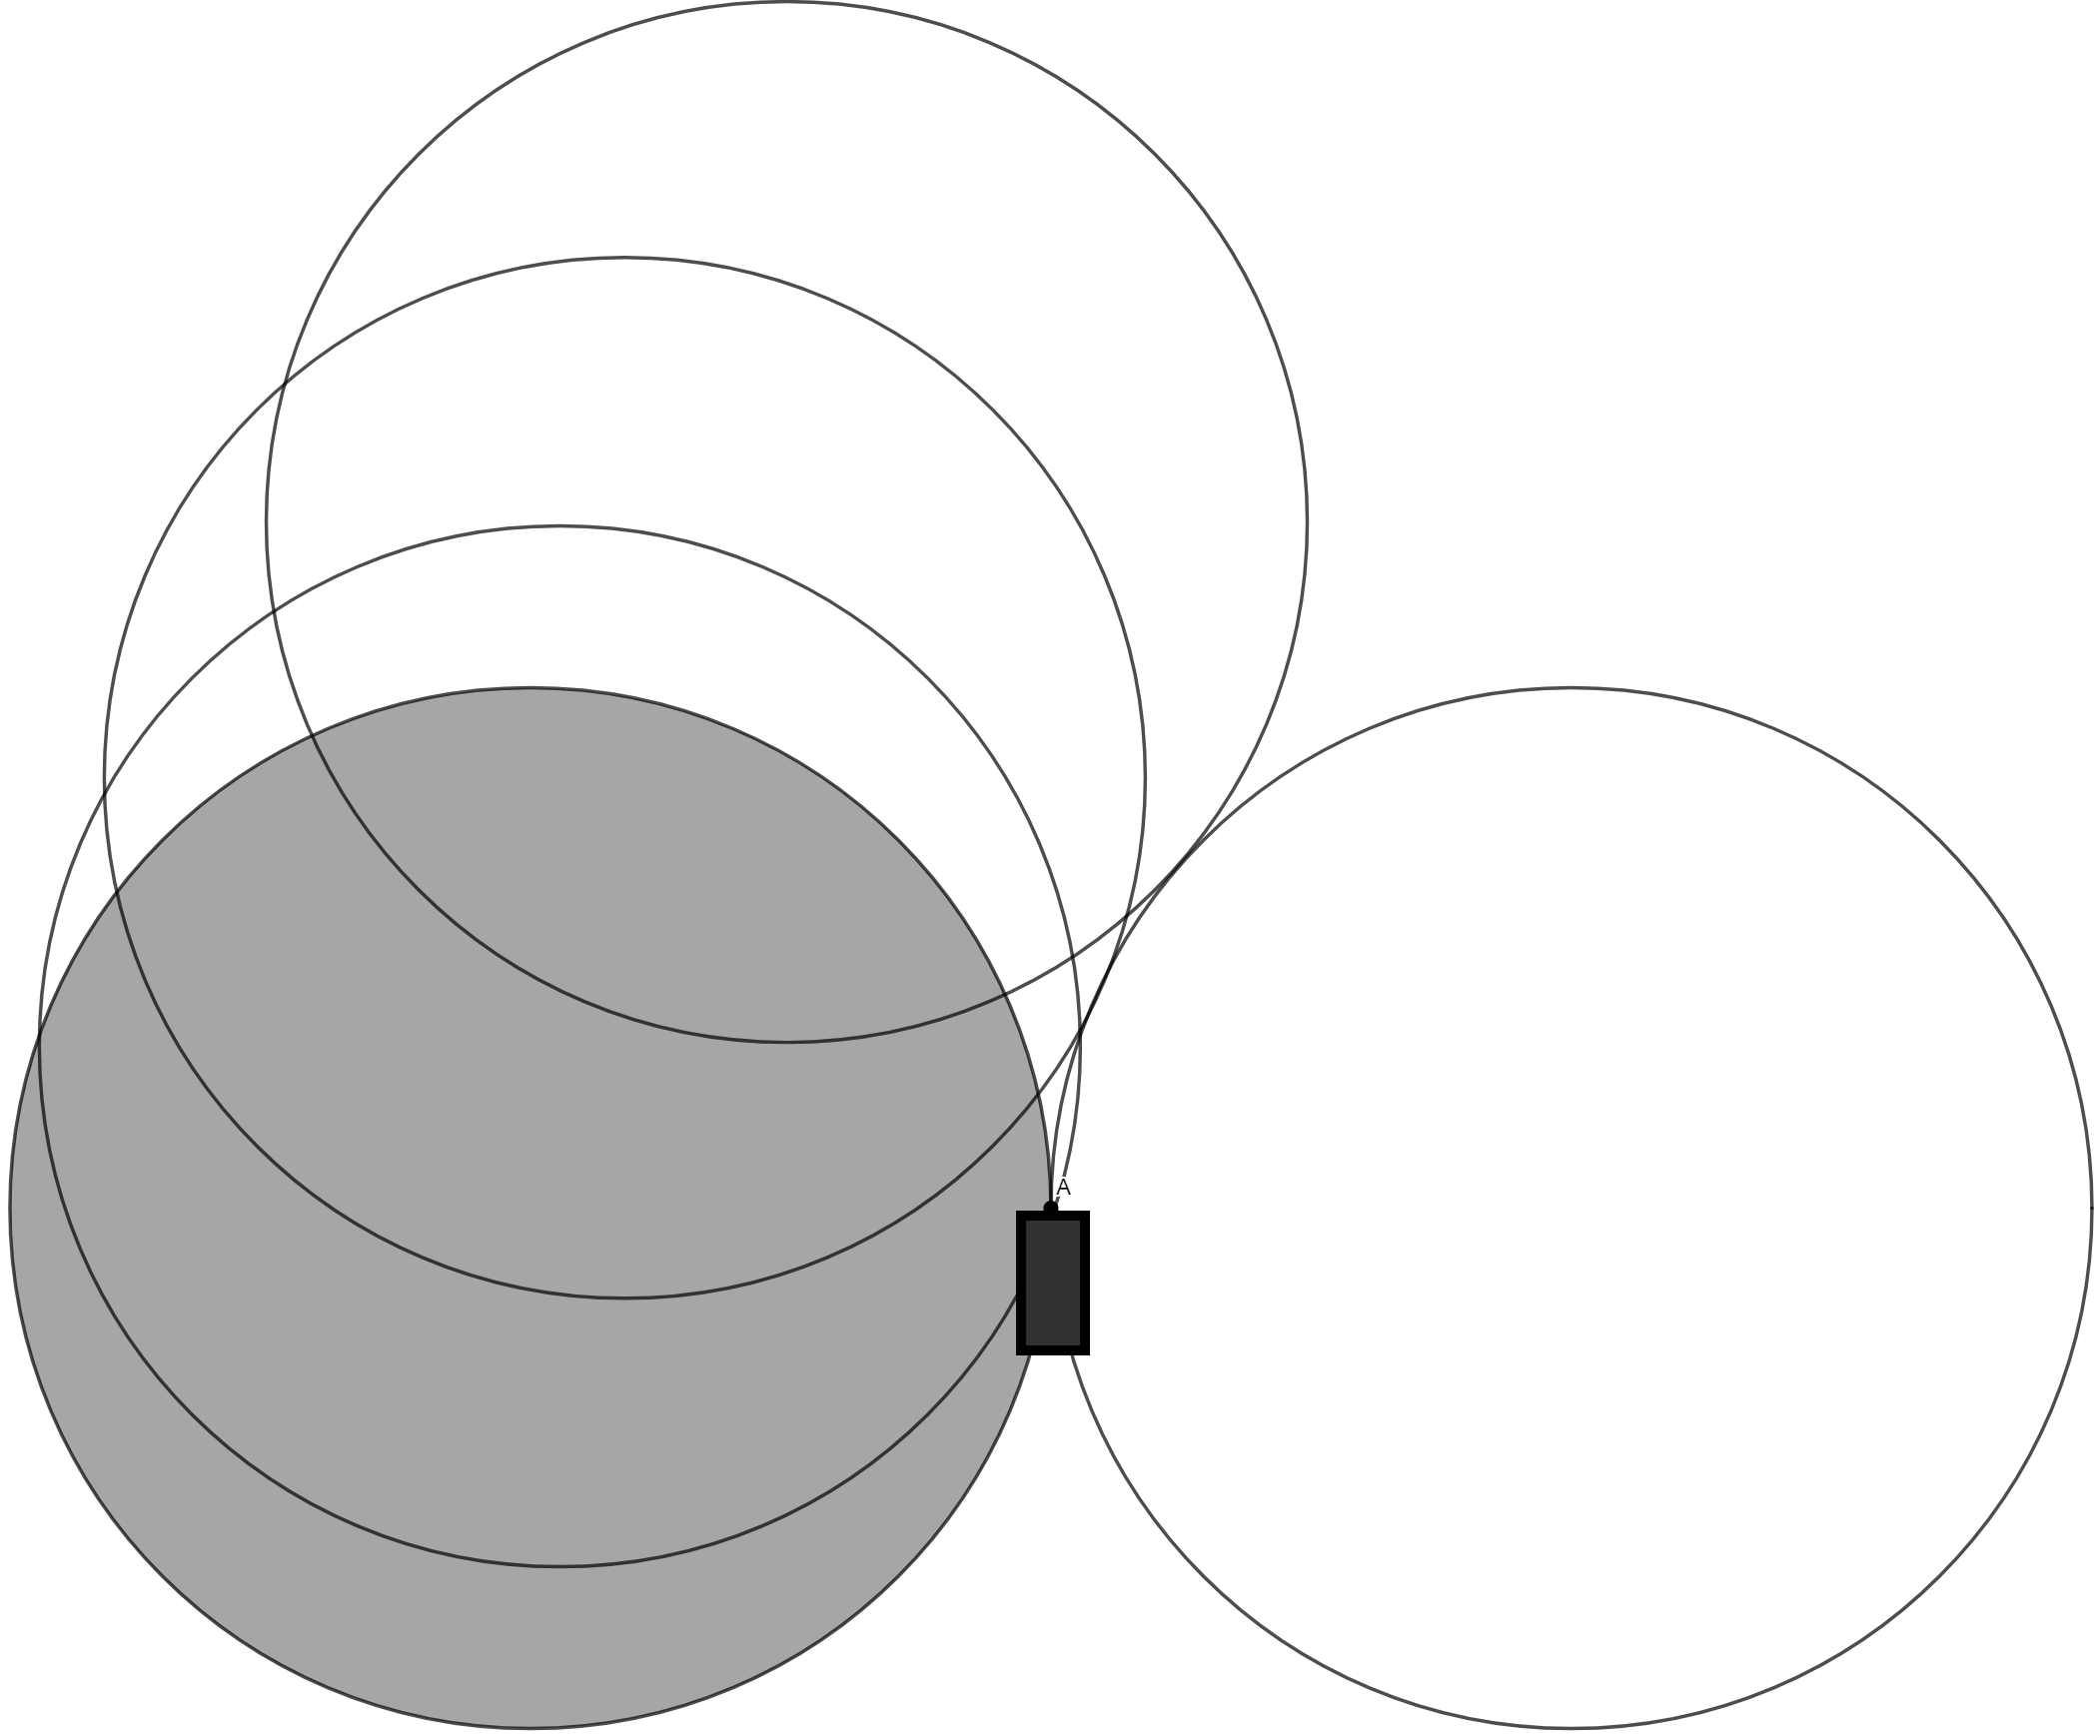
\includegraphics[scale=0.12]{images/it_can2.png}
    \caption{La figure de gauche illustre une représentation très simplifiée du fait que l'électron peut progresser n'importe où dans le plan (d'un principe similaire au \textbf{Théorème 3.4}). Les parties colorées représentent la surface que l'électron peut traverser, jusqu'à $n_{bouton}=3$. Le changement de couleur selon les cercles alignés
    illustre un appui sur le bouton ($n_{bouton} \longmapsto n_{bouton}+1$). \\ La figure de droite illustre le fait qu'il peut aussi trouver un moyen de passer à l'intérieur de n'importe quel cercle trigonométrique.}
  \end{figure}

  On comprend donc à travers ces représentations que l'électron peut progresser n'importe où dans le plan, même avec une orientation fixée.

\end{proof}

\begin{theorem}
  Il est possible de retarder le trajet de l'électron.
\end{theorem}

\begin{proof}
  En considérant la possibilité de laisser l'électron effectuer plusieurs trajets circulaire (des cercles), puis à un moment de donné de reprendre son trajet, nous savons déjà que nous pouvons retarder l'électron. Voici une illustration:

  \begin{figure}[H]
    \centering
    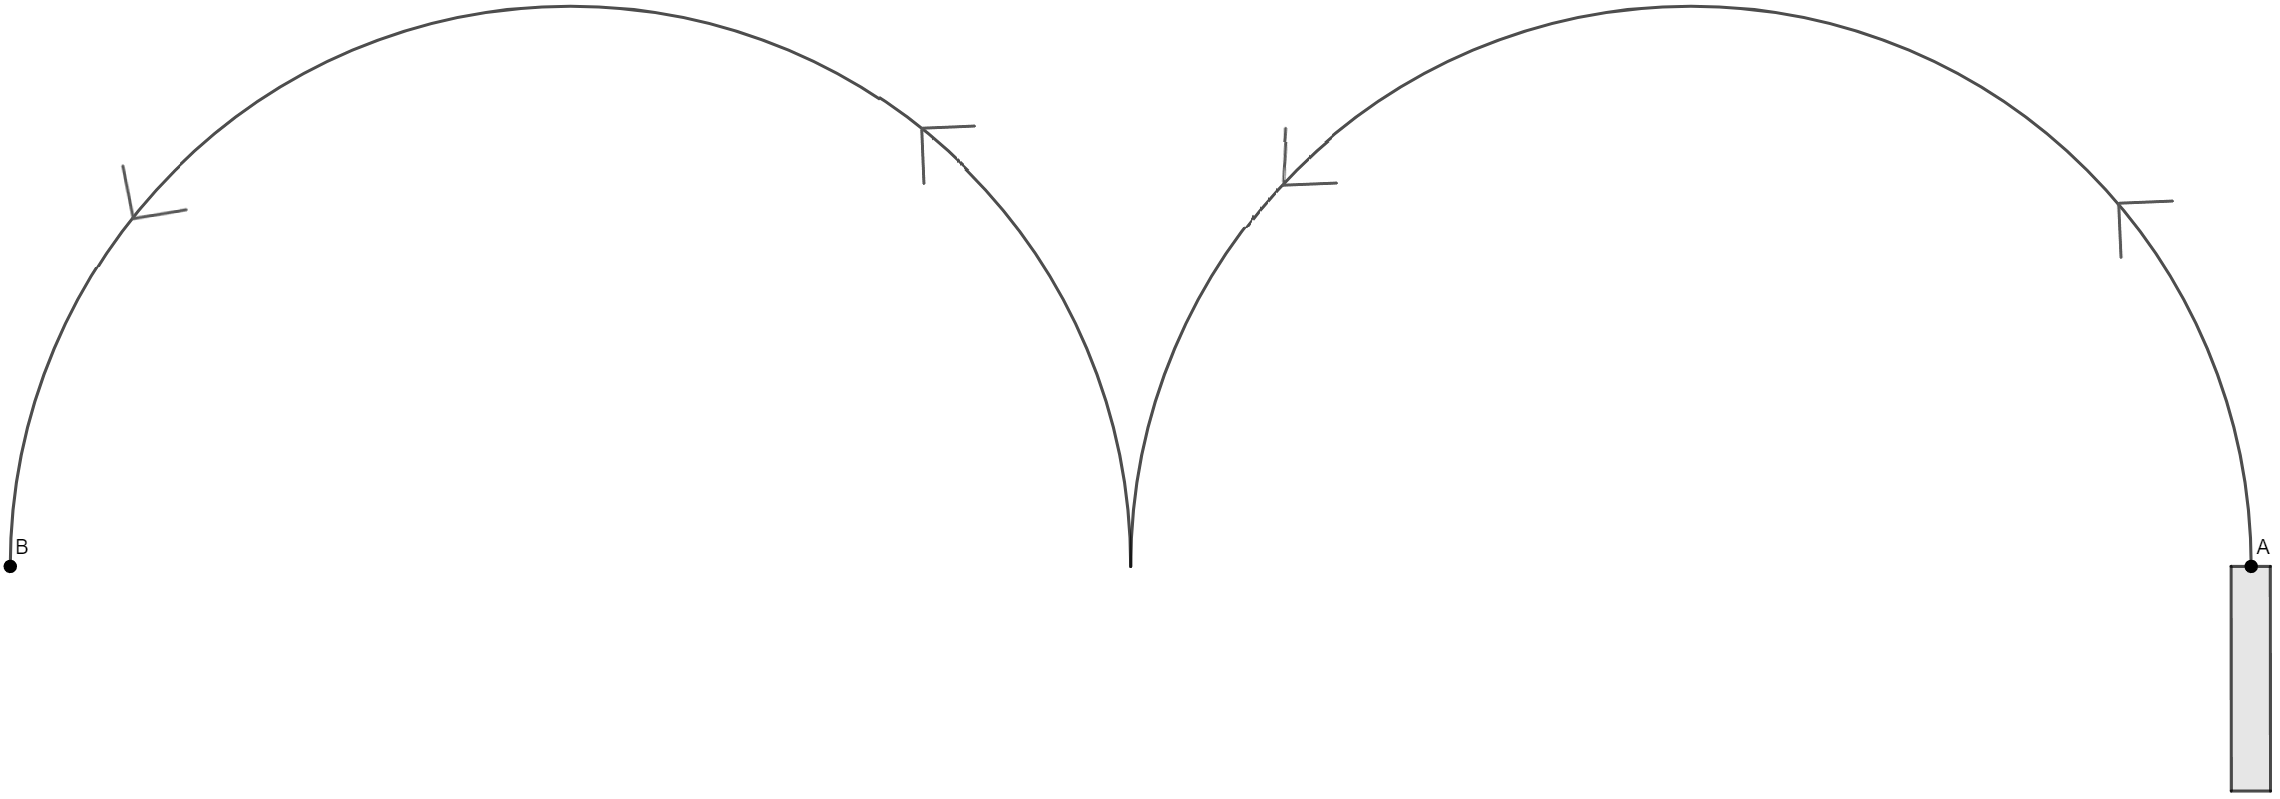
\includegraphics[scale=0.14]{images/not_long.png}
    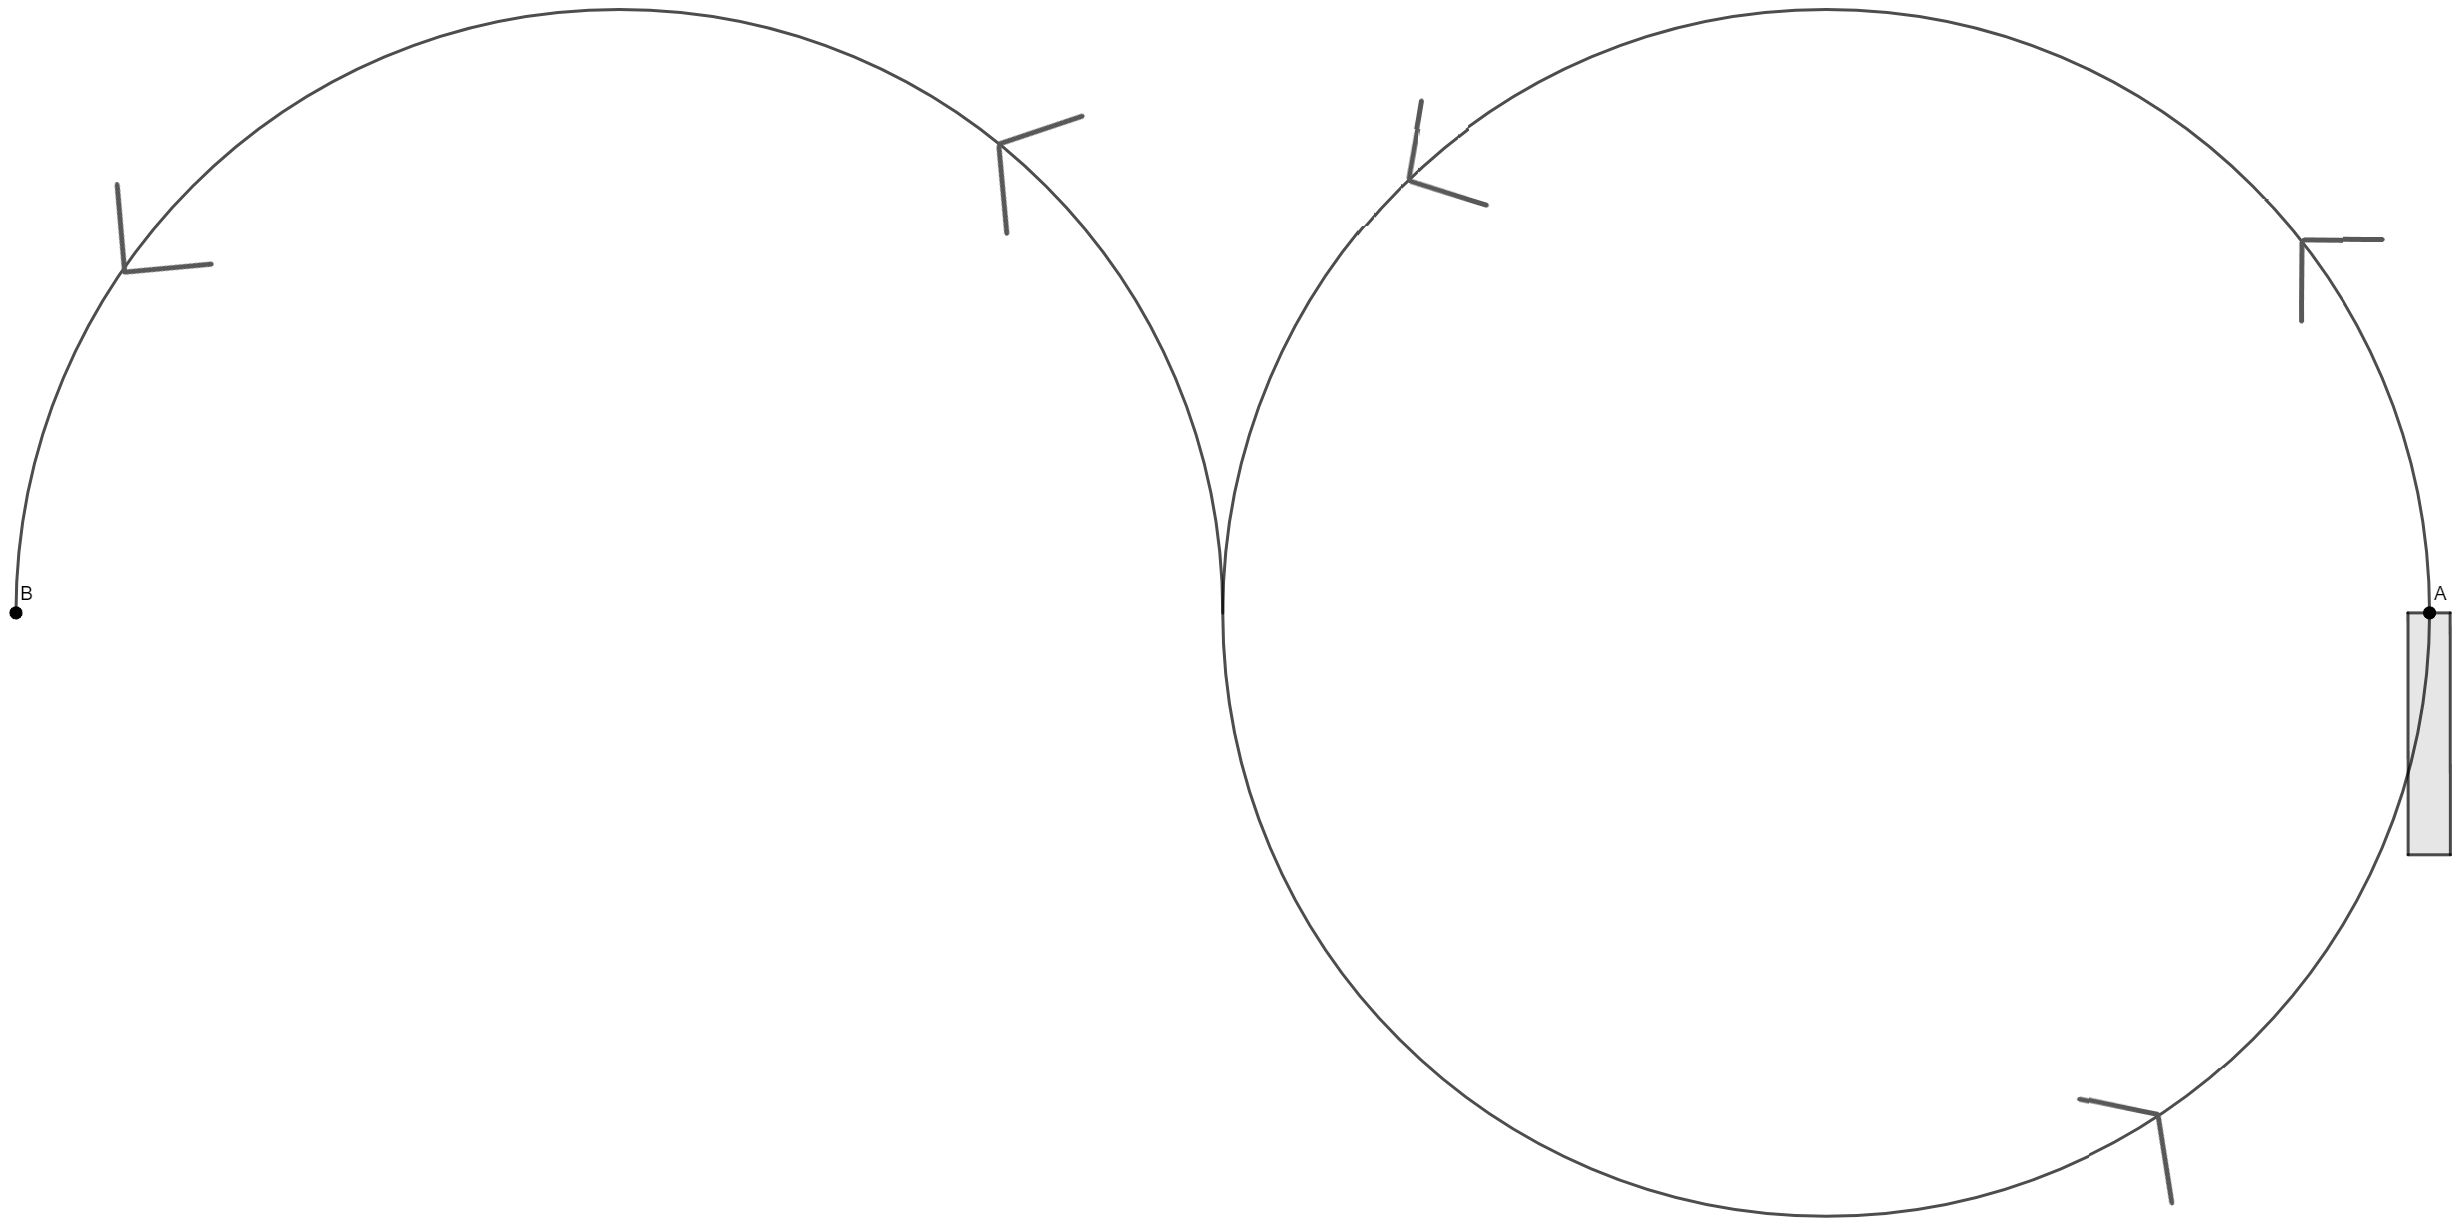
\includegraphics[scale=0.13]{images/really_long.png}
    \caption{Les points $A$ et $B$ sont situés au même emplacement dans le plan. On remarque bien que le trajet de la figure du bas est plus longue que le trajet de la figure du haut. Ces figures montre un retard de l'électron du bas par rapport à celui du dessus égal à $2\pi$.}
  \end{figure}

  On comprend accessoirement que l'on peut retarder l'électron par des multiples de $2\pi$ en laissant l'électron former des cercles comme on le souhaite sur place, ou en appuyant encore sur des boutons, comme le montre la figure ci-dessous:

  \begin{figure}[H]
    \centering
    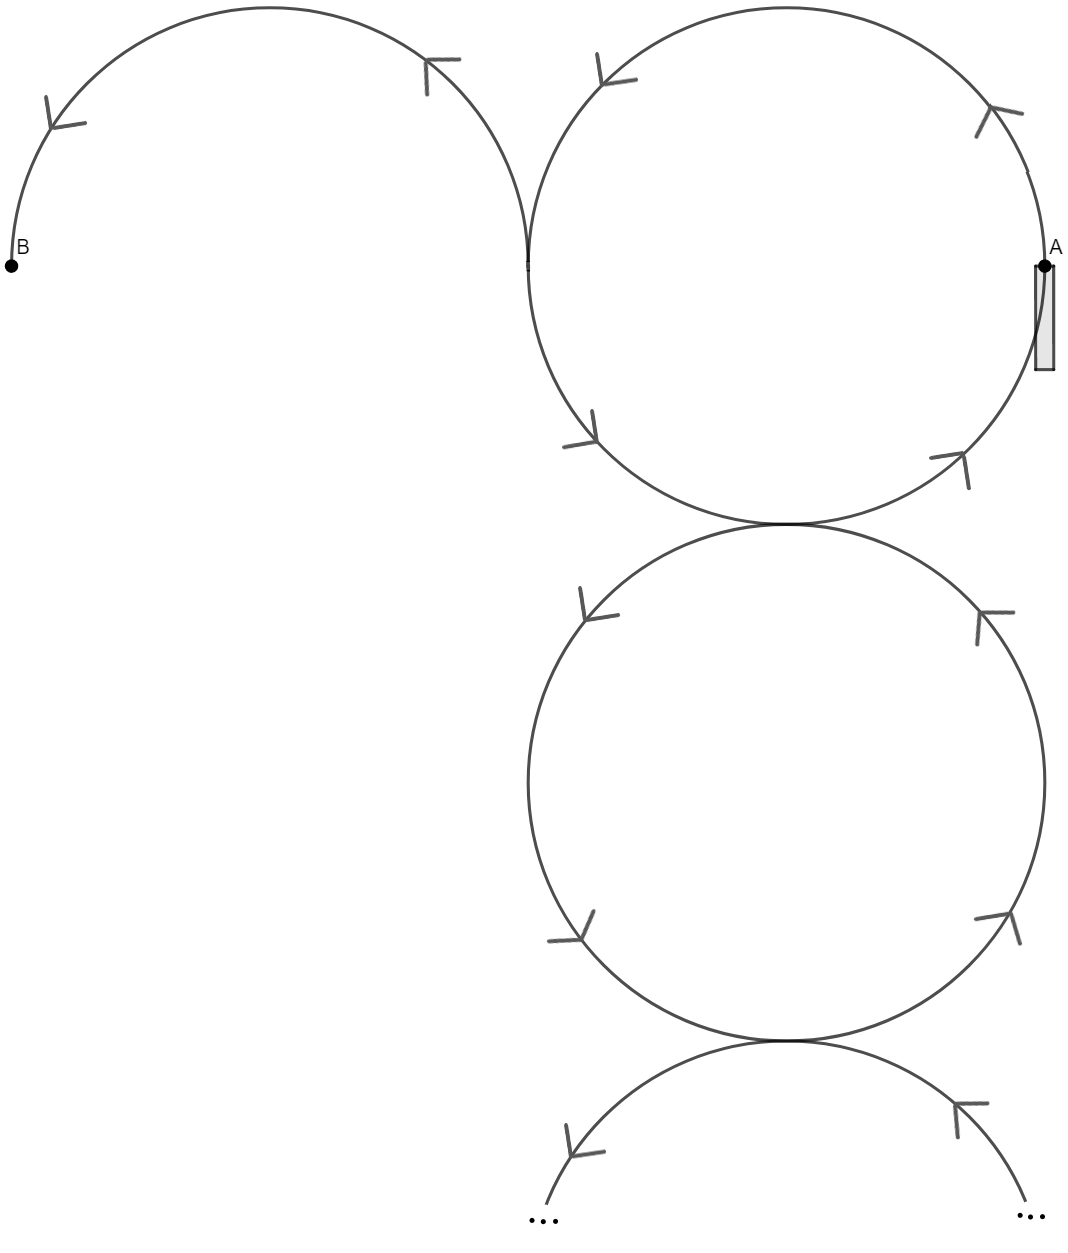
\includegraphics[scale=0.2]{images/make_it_longer.png}
    \caption{On appuie sur le bouton afin de faire partir l'électron vers le bas, puis on le fait revenir sur son trajet initial.}
  \end{figure}

  Jusque-là nous avons démontré des retards étant des multiples de $2\pi$. Cependant, nous remarquons que selon le trajet, nous pouvons tout de même retarder l'électron sans que ce retard soit un multiple de $2\pi$. Voici un exemple:

  \begin{figure}[H]
    \centering
    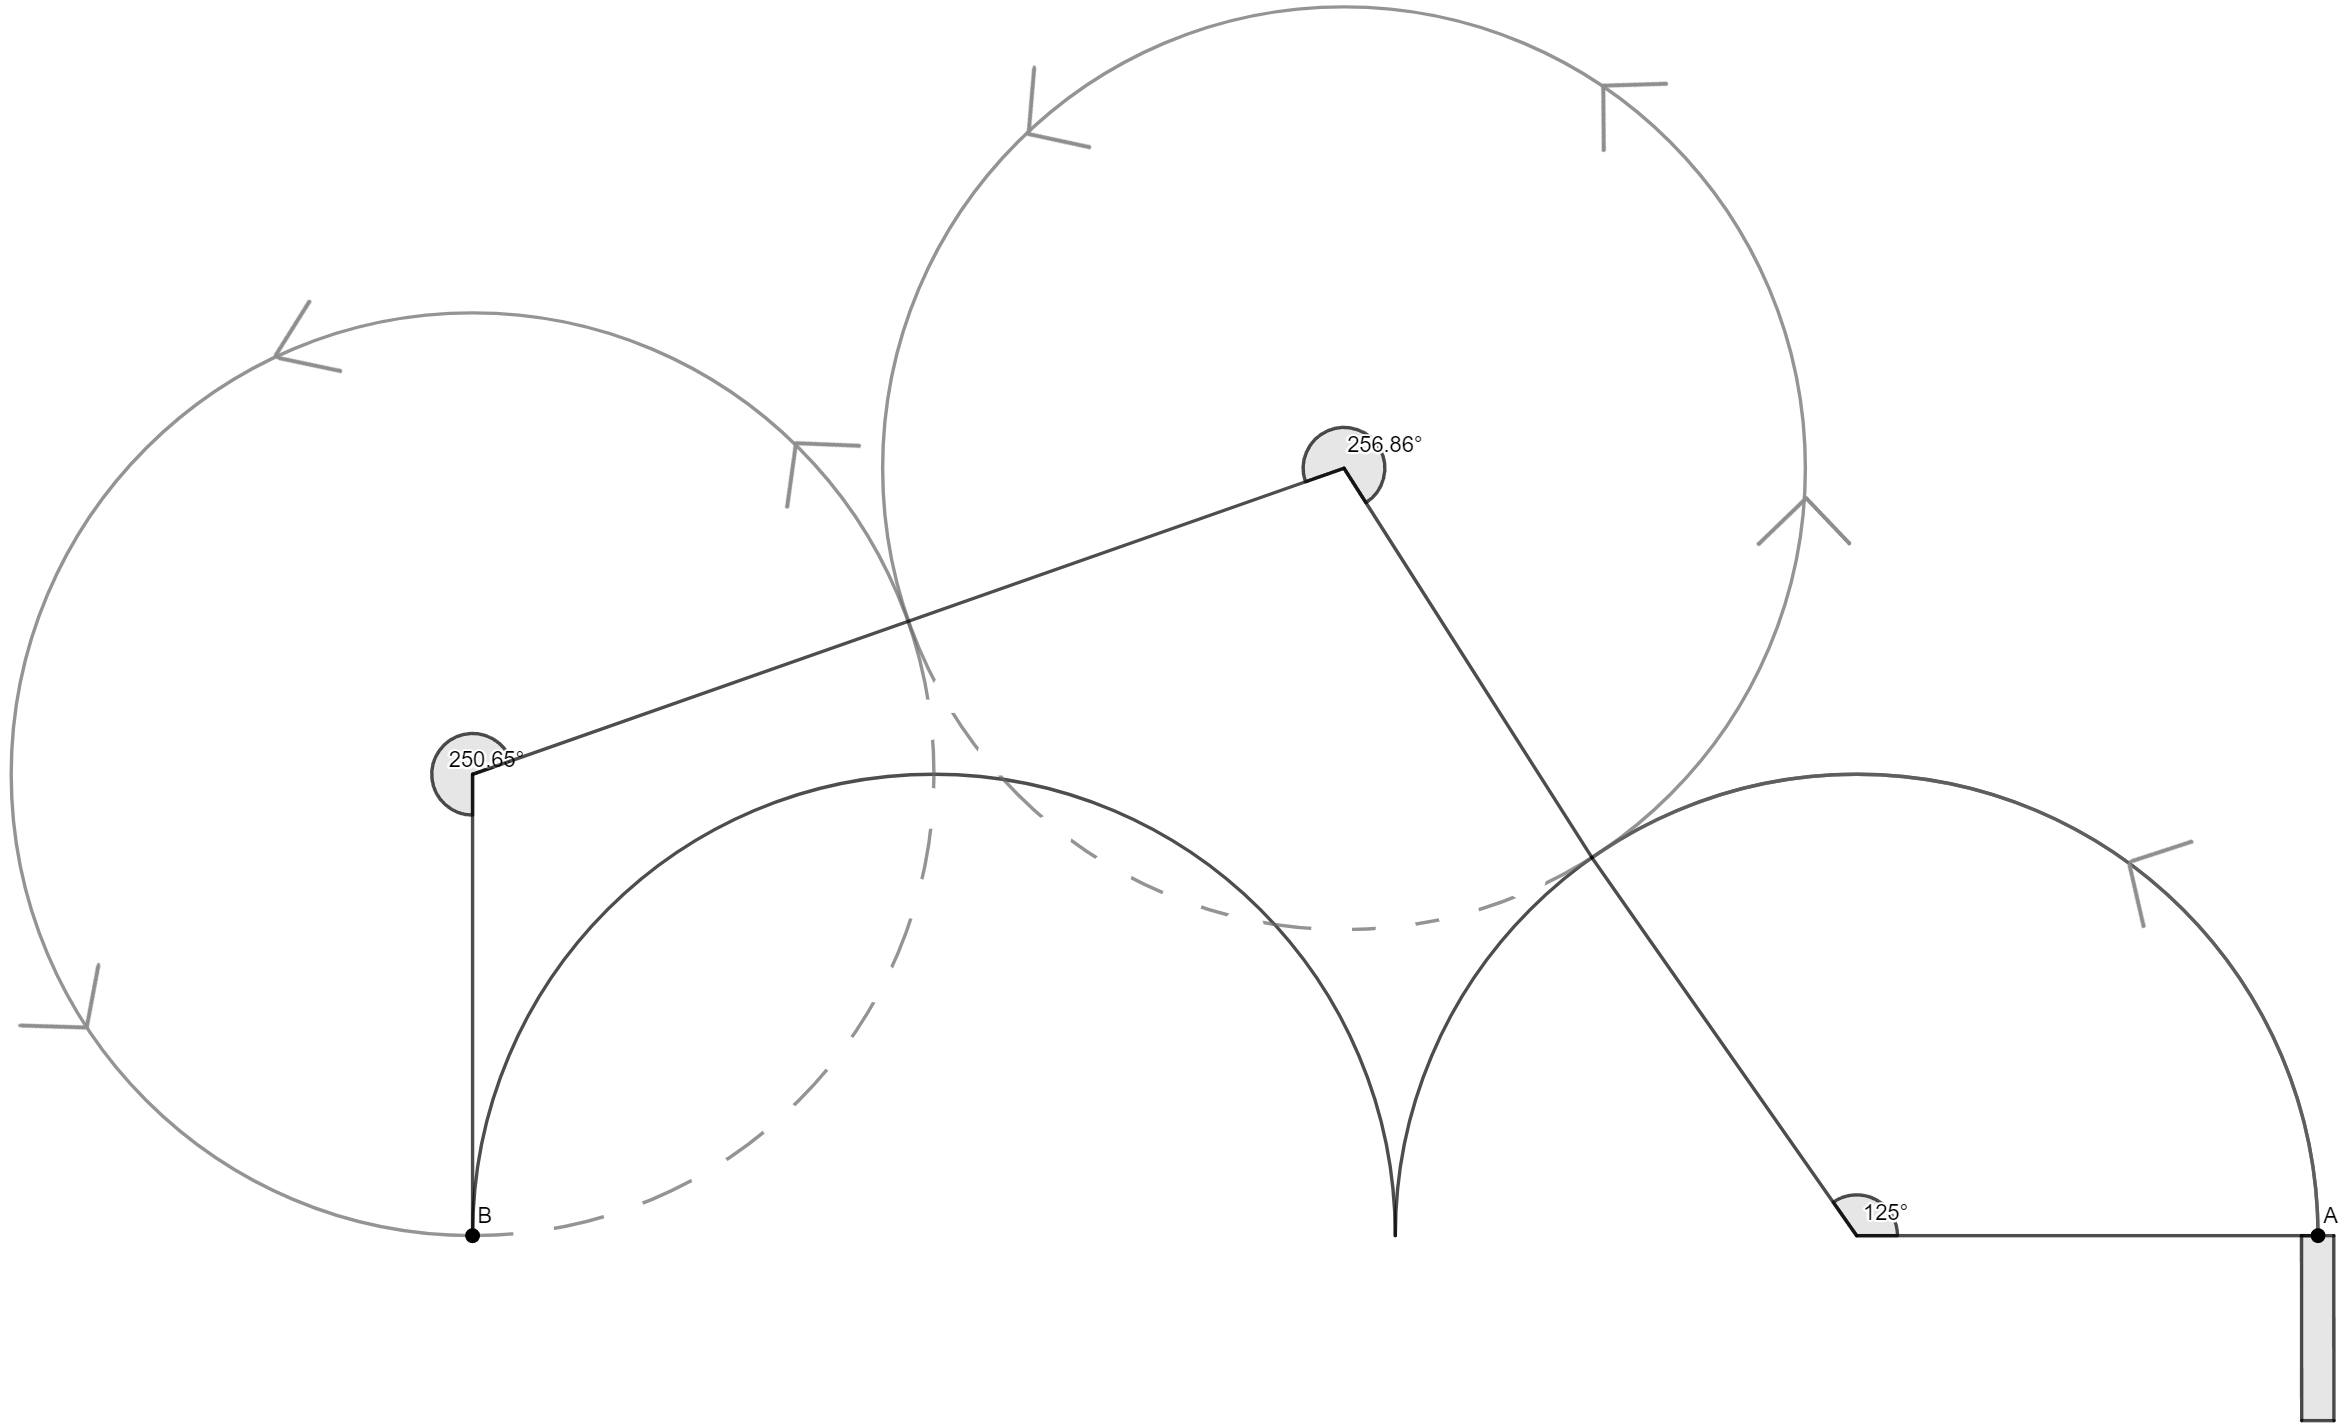
\includegraphics[scale=0.205]{images/not_a_multiple_of_pi.png}
    \caption{Le même trajet que celui des figures du dessus, à l'exception du rajout d'un autre moyen d'atteindre $B$. On note cet autre trajet $T$. Nous avons \[T=\frac{\pi(125°+256.86°+250.65°)}{180°}=\frac{63251\pi}{18000}\approx 11.040\] 
    On comprend que ce nombre n'est pas divisible par $2\pi$.}
  \end{figure}

  On en conclut qu'il est certainement possible de retarder l'électron avec un retard souhaité (et non pas forcément un multiple de $2\pi$).

\end{proof}

\section{Réponse à la Question 4}


Un raisonnement sur l'emplacement des électrons nous induit l'idée que Nicolas peut toujours faire en sorte que, après un certain temps, les k électrons se trouvent au
même endroit au même moment. Selon le \textbf{Théorème 9.1}, Nous savons dors-et-déjà que l'on peut amener l'électron n'importe où, même avec une orientation fixée. Comme l'explique le \textbf{Théorème 9.2}, nous pouvons aussi 
le retarder. On suppose donc que l'on peut toujours faire croiser les électrons au même endroit, au même moment. 

\section{Théorèmes pour la Question 5}

\textit{Remarque.} Il n'a pas été précisé dans l'énoncé, mais nous prendons des valeurs $\forall M\in\mathbb{N}, M>2$, car nous considérons qu'un segment n'est pas un polygone régulier. 

\begin{theorem}
    Pour $M=3$, le polygone régulier à $M=
    3$ côtés dont les sommets sont sur un cercle de rayon $r=1$ est admirable.
\end{theorem}

\begin{proof}
    Prenons le cas où le canon est au milieu d'un des côtés composant le polygone régulier à $M$ côtés. Ayant le triangle inscrit dans un cercle de rayon $r=1$, nous avons la formule:

    \[r=\frac{c}{3}\sqrt{3} \Leftrightarrow c=\sqrt{3}r \implies c=\sqrt{3}\]
    Avec $c\in\mathbb{R^+}$, la longueur des côtés du triangle équilatéral.

    On appelle $B,D,C$ les sommets du triangle équilatéral. Nous avons donc le milieu de $BD=\frac{c}{2}=\frac{\sqrt{3}}{2}$. On appelle $I$ le milieu de $BD$, $O$ le milieu de $BC$ et $P$ le milieu de $DC$. 

    Si l'on souhaite représenter les tangentes sur les arcs de cercles aux points $I,O,P$, nous remarquons que l'angle séparant ces tangentes face aux côtés du triangle $BDC$ sont égaux. En d'autres termes, les angles d’incidence et de réflexion par rapport au arcs de cercles sont les mêmes.

    \begin{figure}[H]
      \centering
      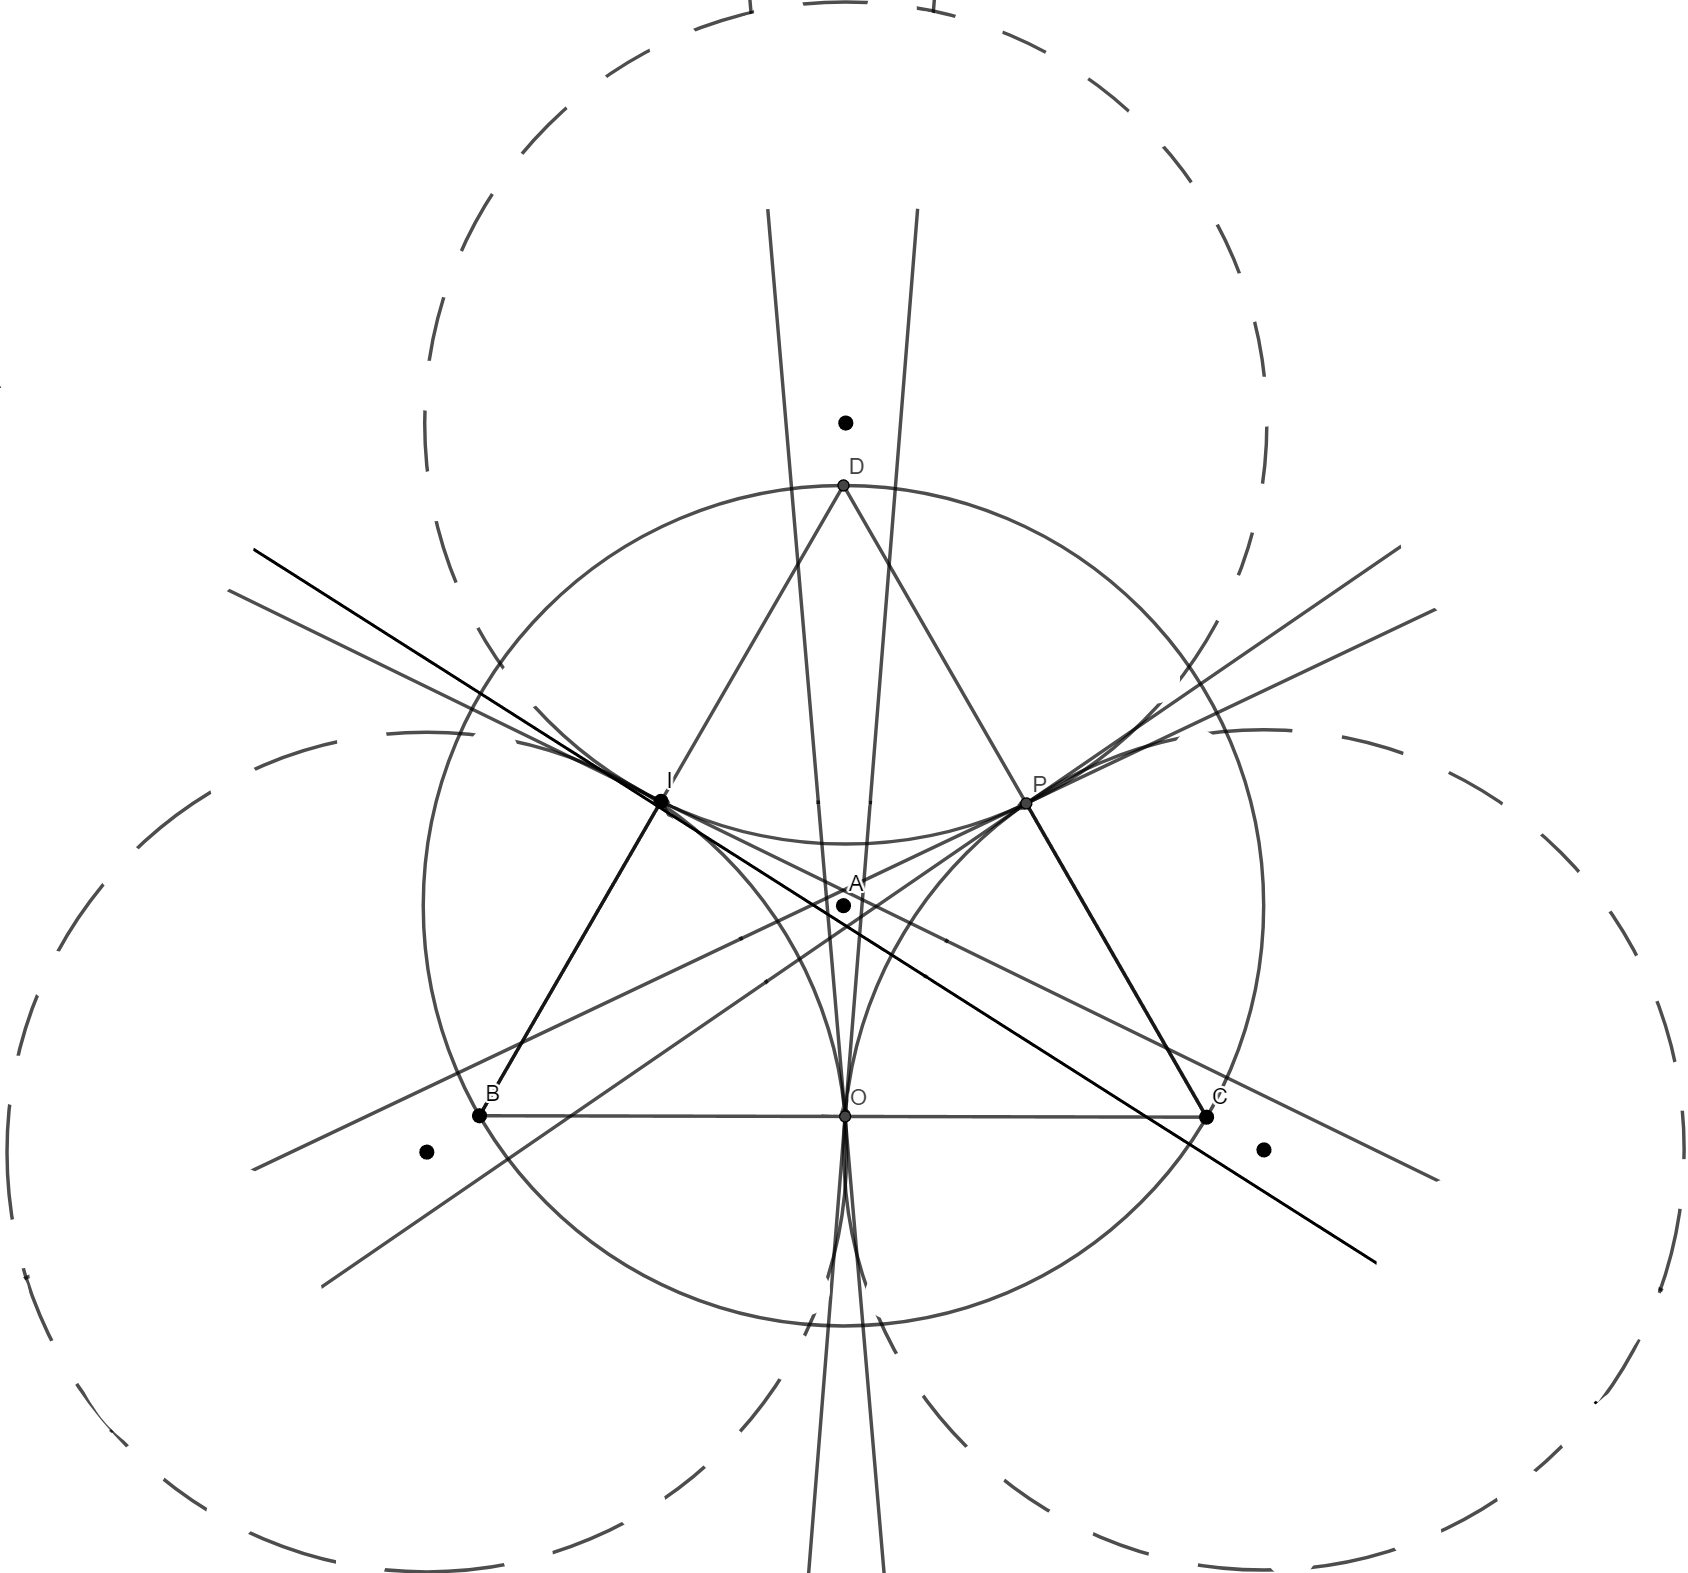
\includegraphics[scale=0.15]{images/q5_tangentes.png}
      \caption{Triangle inscrit dans un cercle de rayon $r=1$ avec les tangentes représentées.}
  \end{figure}

  On en déduit que le trajet démarrant au milieu d'un des côtés peut être un trajet périodique. Cela implique aussi que le polygone 
  régulier de côtés $M=3$ est admirable, car, peut importe la numérotation attribuée, nous avons trouvé un trajet qui satisfait tous les cas.
\end{proof}

\section{Réponse à la Question 5}

Actuellement, selon le \textbf{Théorème 11.1}, nous avons trouvé que le polygone régulier à 3 côtés est admirable.






















































\newpage
\section{Annexe}

\begin{theorem}
  Soit $f$ une fonction continue tel que $f:\mathbb{R}\longrightarrow \mathbb{R}, x\longmapsto f(x)$, $f$ étant définit dans un repère orthonormé. Soit $a,b\in\mathbb{R}$. On considère la longueur de la courbe de $f$ allant de $a$ à $b$ étant égale à:

  \[\lambda(a,b)=\int_{a}^{b} \sqrt{1+{f^\prime}(x)^2} \,dx\]
\end{theorem}

\begin{proof}
  En se basant sur la définition d'une intégrale, qui est la somme de grandeurs infiniment petites, que l'on note $dx$ (différence de $x$ infiniment petite d'une fonction continue $f$ associant une image $f(x), \forall x\in I$ avec $I=[a,b]$), on peut considérer la longueur de la courbe semblable à la représentation ci-dessous: 
  
  (On note $dx$ une différence de $x$ infiniment petite et $df$, une différence infiniment petite d'images).

  \begin{figure}[H]
    \centering
    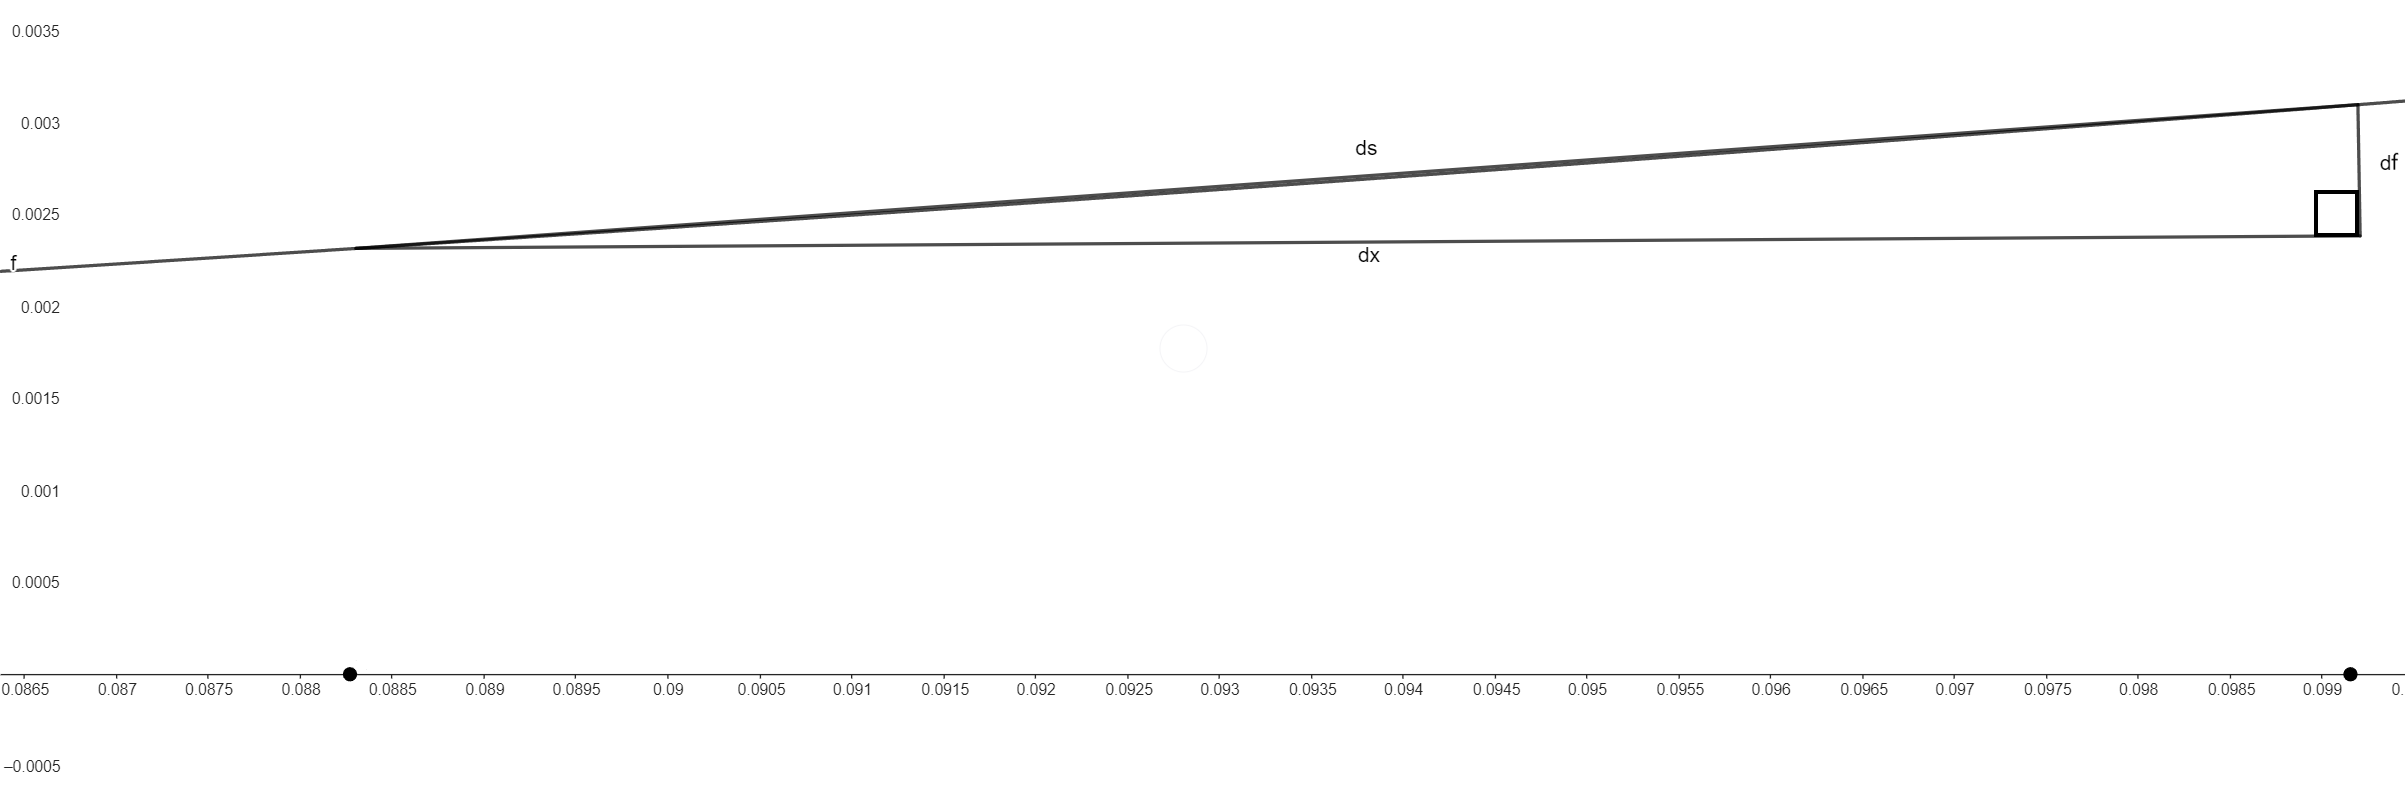
\includegraphics[scale=0.2]{images/curve.png}
    \caption{L'exemple choisi a été pour la courbe de $f(x)=x^{\frac{5}{2}}$.}
  \end{figure}

  C'est donc la somme de segments infiniment petits ($ds$) qui nous donne la longueur de la courbe de $f$. Soit donc:

  \[\lambda(a,b)=\int_{a}^{b}ds\]

  Étant dans un repère orthonormé, nous savons que le triangle formé à partir de $ds, dx$ et $df$ est rectangle. Soit donc, d'après le Théorème de Pythagore:

  \[(ds)^2=(dx)^2+(df)^2 \Leftrightarrow ds=\sqrt{(dx)^2+(df)^2}\]

  (On ne considère pas la racine négative étant donné qu'une longueur est toujours positive).

  Factorisons par $(dx)^2$ au sein de notre égalité afin de faire apparaître $f^\prime(x)$.

  \[ds = \sqrt{(dx)^2(1+(\frac{df}{dx})^2)} \Leftrightarrow ds = \sqrt{1+(\frac{df}{dx})^2}dx\]

  (Cela fonctionne car $dx\ne0$, $dx\to 0$).

  On reconnait le fait que par définition, $f^\prime(x)=\frac{df}{dx}$. Soit donc: 

  \[ds=\sqrt{1+{f^\prime}(x)^2}dx \implies \lambda(a,b)=\int_{a}^{b}\sqrt{1+{f^\prime}(x)^2}dx \Leftrightarrow \lambda(a,b)=\int_{a}^{b}\sqrt{1+{f^\prime}(x)^2}\,dx\]
\end{proof}

\begin{theorem}
  Soit $a,b\in\mathbb{R}$ avec $b>a$. Soit $f,g$ deux fonctions continues sur $[a,b]$ avec $f:\mathbb{R}\longrightarrow \mathbb{R}, x\longmapsto f(x)$ et $g:\mathbb{R}\longrightarrow \mathbb{R}, x\longmapsto g(x)$. Si $f(x)\geq g(x) \forall x\in[a,b]\implies$

  \[\int_{a}^{b}f(x) \,dx \geq \int_{a}^{b}g(x) \,dx\]
\end{theorem}

\begin{proof}
  Puisque $f(x)\geq g(x), \forall x\in[a,b] \implies f(x)-g(x)\geq 0\forall x\in[a,b] $. Par le théorème fondamental de l’analyse, si $f(x)$ est continue sur $[a,b]$, alors son intégrale $F(b)-F(a)$ sur $[a,b]$ est définie comme :
  \[F(b)-F(a) = \int_{a}^{b} f(x) \,dx\]

  De même, l'intégrale de $g$, $G(b)-G(a)$, est définie comme: \[G(b)-G(a) = \int_{a}^{b} g(x) \,dx\]

  On sait aussi que $f(x)-g(x)\geq0$. Cela implique que l'aire en dessous de cette différence est supérieure à zéro. Intégrons cette inégalité de $a$ à $b$: \[\int_{a}^{b} f(x) - g(x), dx \geq 0 \Leftrightarrow F(x)-G(x) \Biggr|_{a}^{b}\geq0 \Leftrightarrow F(b)-G(b) -(F(a)-G(a)) \geq 0 \]

  Soit donc:

  \[F(b)-F(a) \geq G(b)-G(a) \Leftrightarrow \int_{a}^{b}f(x) \,dx \geq \int_{a}^{b}g(x) \,dx\]
\end{proof}

\begin{theorem}
  Soit $A,B$ deux points dans un plan quelconque. Le trajet le plus court de $A$ à $B$ est une ligne droite.
\end{theorem}

\begin{proof}
  Considérons deux points $A,B$ dans un plan quelconque. Soit le repère orthonormé $(A;I;J)$ tel que \overrightarrow{AJ} $\perp$ \overrightarrow{AB}. On considère donc les points $A(x_A=0,y_A=0)$ et $B(x_B,y_B=0)$.

  Soit $f_q, f_q:\mathbb{R^+}\longrightarrow \mathbb{R^+}, x\longmapsto f_q(x)$, une fonction continue sur $[x_A,x_B]$ modélisant le trajet de $A$ à $B$ (n'étant pas une droite, avec $f_q(x)=0$ nécessairement à $x_A$ et $x_B$, pour compléter la courbe). Soit $f_k, f_k:\mathbb{R^+}\longrightarrow \mathbb{R^+}, x\longmapsto 0$ une fonction
  continue sur $[x_A,x_B]$ modélisant la droite entre $A$ et $B$.

  En effectuant un raisonnement par l'absurde, supposons que $f_q(x_A)=f_q(x_B)=0$ mais non $f_q(x)=0 \forall x\in\mathbb{R}$ (en d'autres termes, $\exists x_p$ (au moins un $x_p$ ou plus) tel que$f_q(x_p)\ne0$), avec $\lambda_q(A,B) < \lambda_k(A,B)$.

  $0$ étant une constante, on sait que ${f_k}^\prime(x)=0$:

  \[\lambda_k(A,B)=\int_{x_A}^{x_B}1 \,dx \Leftrightarrow \lambda_k(A,B)=x\Biggr|_{x_A}^{x_B} \Leftrightarrow \lambda_k(A,B)= x_B-x_A \Leftrightarrow \lambda_k(A,B)= x_B\]

  Or $\exists x_p$ tel que$f_q(x_p)\ne0$, impliquant que $f_q(x)$ doit avoir une valeur dépendant de $x$ (et non pas juste d'une constante $k$ ou $kx, k\in\mathbb{R^*}$, car dans un tel cas, $f_q(x_A)\ne f_q(x_B)$).

  \[\lambda_q(A,B)=\int_{x_A}^{x_B}\sqrt{1+f_q{^\prime}(x)^2} \,dx\]

  Nous savons donc que:

  \[1 \leq \sqrt{1+f_q{^\prime}(x)^2}\]

  $\forall x \in \mathbb{R}$ car $f_q{^\prime}(x)^2\geq 0, \forall x \in \mathbb{R}$, avec la fonction racine carré étant croissante sur $\mathbb{R}$.

  \[\int_{x_A}^{x_B}1 \,dx \leq \int_{x_A}^{x_B}\sqrt{1+f_q{^\prime}(x)^2} \,dx\]

  (D'après le \textbf{Théorème 13.2}).

  Or $\exists x_p$ tel que $f_q(x_p)\ne0 \implies {{f_q}^\prime(x_p)}^2>0$. Par conséquent, on comprend bien que $\int_{x_A}^{x_B}\sqrt{1+f_q{^\prime}(x)^2} \,dx$, étant une somme infinie (la convergence de la somme de Riemann), cette somme doit admettre nécessairement à la valeur $x_p$, $1<\sqrt{1+{f_q{^\prime}(x_p)}^2}$. On en déduit que:

  \[ \int_{x_A}^{x_B}1 \,dx < \int_{x_A}^{x_B}\sqrt{1+f_q{^\prime}(x)^2} \,dx\]

  Soit donc $\lambda_k(A,B) < \lambda_q(A,B)$, soit le trajet le plus court pour aller de $A$ à $B$ étant une ligne droite.
\end{proof}
\end{document}